% % Objetivo del archivo: actuar como archivo raíz para centralizar la configuración, carga de paquetes, especificaciones de la estructura y carga de archivos de redacción.
%
%--------------------------------------------------------------------------
%COD	CLASE DE \LaTeX
%--------------------------------------------------------------------------
\documentclass[12pt,a4paper,oneside]{report}
% Sintaxis:
%\documentclass[TAMAÑO-DE-LETRA, FORMATO-HOJA, COLUMNAS, CARILLAS, NUEVO-CAPITULO, MODO-TITULO, APAISADO, ALINEAR-ECUACIONES, MODO-BORRADOR]{TIPO}
%	TAMAÑO-DE-LETRA: tamaño de la tipografía en puntos.
%		Sintaxis: Npt
%			N: número
%			pt ; indica la unidad 'punto tipográfico'.
%	FORMATO-HOJA: tamaño de la hoja del \LaTeX. Argumentos válidos típicos (consultar web para más info): a4paper, letterpaper, a5paper, b5paper, legalpaper.
%	COLUMNAS: imprimir a una o dos columnas. Argumentos válidos: onecolumn, twocolumn.
%	CARILLAS: imprimir a una o dos carillas; a dos altera la simetría de los márgenes entre páginas pares e impares. Argumentos válidos: oneside, twoside.
%	NUEVO-CAPITULO: para documentos 'twoside' regula si un nuevo capitulo puede empezar en cualquier página o solo en impares. Argumentos válidos: openany, openright.
%	MODO-TITULO: indica si el título del \LaTeX debe ir en una página propia, o en la misma en la que empieza el texto. Argumentos válidos: notitlepage, titlepage.
%	APAISADO: no modifica los márgenes, por lo que es mejor emplear el paquete pdflscape. Argumento válido: landscape.
%	ALINEAR-ECUACIONES: por defecto las ecuaciones se centran y se numeran a la derecha; para cambiarlo se admiten hasta dos argumentos:
%		fleqn: formulas alineadas a la izquierda.
%		leqno: etiquetas alineadas a la izquierda.
%	MODO-BORRADOR: acelera la compilación al no cargar las imágenes, sustituyéndolas por un recuadro de tamaño equivalente y otros detalles. Argumentos válidos: draft, final.
%
%	TIPO: tipo de LaTeX. Argumentos válidos típicos (consultar web para más info):
%		report: LaTeX largos; tipo tesis académica.
%		book: libros.
%		article: artículos.
%
%	No todas las opciones son obligatorias, y la mayoría contienen un valor por defecto.
%--------------------------------------------------------------------------
%COD	FUENTE Y GEOMETRÍA
%--------------------------------------------------------------------------
% Objetivo del archivo: definir la fuente de la letra; definir márgenes de página; definir espacios.
%
% Listado de unidades de espacios disponibles en latex:
%pt: punto tipográfico; 1pt=0,3515 mm.
%mm: milímetro.
%cm: centímetro.
%in: pulgada.
%ex: altura de una <<x>> en la fuente activa.
%em: ancho de una <<M>> en la fuente activa.
%mu: (em/18) de la fuente activa en modo $$.
%sp: puntos especiales; 65536sp = 1pt.
%
%COD FUENTE
% La fuente se define mediante la carga del paquete específico de cada fuente. Consultar en internet las fuentes disponibles y sus nombres en latex. Por ejemplo, {helvet} es el equivalente a Arial (que es una fuente propietaria).
\usepackage{helvet}
\renewcommand{\familydefault}{\sfdefault}% Eliminar serif.
%
%COD MÁRGENES DE PÁGINA
% Los márgenes se definen mediante la carga del paquete {geometry} que permite establecer los márgenes de cada lado de la página.
\usepackage[left=2cm,right=2cm,top=2cm,bottom=2cm]{geometry}% Multitud de opciones y configuraciones.
% Sintaxis:
%\usepackage[LADO=VALOR]{geometry}
%	LADO: lado de la hoja del que se define el margen.
%		Posibles valores: left, right, top, bottom.
%	VALOR: dimensión del margen expresada como combinación de un argumento numérico (x) y su unidad (u).
%		Sintaxis: xu
%			x: valor numérico del espacio de margen.
%			u: unidad de medida del espacio de margen.
%				Posibles valores: cm, pt.
%	geometry: nombre del paquete.
%
%COD INTERLINEADO
\linespread{1.2}
% Sintaxis:
%\linespread{x}
%	x: valor numérico, en pt.
% Como orientación: {1pt}=valor por defecto ; {1.3}=linea y media ; {1.6}=doble espacio.
%
%COD IDENTACIÓN DE PRIMERA LÍNEA DE PÁRRAFO
\setlength{\parindent}{1cm}
%COD ESPACIADO VERTICAL ENTRE PÁRRAFOS
\setlength{\parskip}{.5cm}
%COD ESPACIADO VERTICAL DE NÚMERO DE PÁGINA A FINAL DE PÁGINA
\setlength{\footskip}{3\baselineskip}
%COD NOTAS AL PIE
% Extender la línea de las notas al pie a todo el ancho de texto de la página.
\renewcommand{\footnoterule}{%
	\kern -3pt
	\hrule width \textwidth height 1pt
	\kern 2pt
}
%
%
%--------------------------------------------------------------------------
%COD	PAQUETES ESTÁNDAR
%--------------------------------------------------------------------------
% Objetivo del archivo: cargar paquetes genéricos con bajo nivel de configuración.
%
%COD CODIFICACIÓN
\usepackage[utf8]{inputenc}
%
%COD TRADUCCIÓN DE LITERALES
% Los literales son los ítems imprimibles generados automáticamente por latex.
% La traducción se hace mediante la carga del paquete {babel}:
\usepackage[spanish]{babel}% Multitud de opciones y configuraciones.
% Sintaxis:
%\usepackage[IDIOMA]{babel}
%	[IDIOMA]: idioma al que queremos traducir.
%	{babeL}: nombre del paquete.
% La traducción por defecto de los literales al castellano es: Index=Índice ; Table=Cuadro ; Figure=Figura.
%
% Se renombran algunos literales para que sean más idiomáticos:
%	Pies de tablas; por defecto: Cuadros; modificado a: Tabla.
\addto\captionsspanish{\renewcommand\tablename{Tabla}}
%	Índice de tablas; por defecto: Índice de cuadros; modificado a: Índice de tablas.
\addto\captionsspanish{\renewcommand\listtablename{Índice de tablas}}
%	Entrada de Referencias en el TOC; por defecto: Referencias; modificado a: .
%\addto\captionsspanish{\renewcommand\bibname{Referencias bibliográficas}}
%	Anexo; por defecto: Apéndice; modificado a: Anexo.
\addto\captionsspanish{\renewcommand\appendixname{Anexo}}
%	Pies de Código; por defecto: Listing; modificado a: Código.
\addto\captionsspanish{\renewcommand\lstlistingname{Código}}
% Índice de Código; por defecto Listing; :modificado a: Índice de Códigos.
\addto\captionsspanish{\renewcommand\lstlistlistingname{Índice de códigos}}
%
%COD MODO CITA
% Para escribir texto formateado al estilo de citas:
\usepackage{csquotes}% Recomendado cargar tras babel.
% Sintaxis de uso en texto:
%	Dos modos de uso:
%
%		a) Entorno: crea un párrafo con el contenido en texto más estrecho y centrado, se emplea invocando en el entorno {displayquote}.
%\begin{displayquote}
%TEXTO
%\end{displayquote}
%
%		b) En línea: introduce las comillas <<>>, se emplea mediante comando.
%\textquote{TEXTO}
%
%	TEXTO: texto que sE mostrará como cita.
%
%COD MATEMÁTICAS
% GENERAL
\usepackage{mathtools}% Basado en el paquete amsmath.
%
% CANCELACIÓN DE TÉRMINOS
\usepackage{cancel}
% Sintaxis de uso en texto:
%	Dos modos de uso:
%
%		a)Cancelar una expresión:
%\cancel{EXPRESIÓN}
%
%		b) Cancelar una expresión e indicar hacia qué término cancela:
%\cancelto{TÉRMINO}{EXPRESIÓN}
%
%	{EXPRESIÓN}: expresión alfanumérica que será cancelada.
%	{TÉRMINO}: valor hacia el que se cancela {EXPRESIÓN}.
%
%COD SÍMBOLOS Y GLIFOS
\usepackage{wasysym,eurosym,amssymb,circledsteps}
%
%OBJETOS Y TABLAS
\usepackage{import,graphicx,rotating,multicol,caption,subcaption,booktabs,multirow,pdfpages}
\usepackage[export]{adjustbox}% Permite añadir un marco a las figuras, con la opción "frame" en el comando de invocación de cada figura.
%\usepackage[table,xcdraw]{xcolor}% Cargar de último por conflictos en el orden de carga.
%
%COD TABLAS
% NOTA: Crear tablas directamente en latex es complicado, se recomienda usar uno de los siguientes métodos:
%
%	A) Usar una web o aplicación que permita crear la tabla con una interfaz tipo hoja de cálculo y que la convierta a código latex, para importarlo. Por ejemplo:
%	http://www.tablesgenerator.com/
%	https://www.latex-tables.com/#
%
%	B) Crear la tabla con otras aplicaciones (editor de textos, hoja de cálculo) y guardarla como una imagen para después insertar esa imagen en el texto englobándola en un entorno de tabla. Mediante un código como:
%
%\begin{table}[H]
%	\begin{figure}[H]
%		\centering
%		\includegraphics[width=1\textwidth, frame]{}
%	\end{figure}
%	\caption{}
%	\label{}
%\end{table}
%
% PERSONALIZACIÓN DE PIES DE FIGURAS Y TABLAS
\captionsetup{textfont={it},labelfont={bf},labelsep=endash,format=hang,justification=raggedright}% Paquete {caption}; multitud de opciones y configuraciones.
%
%COD PDFs
% Los pdf se incluyen con el paquete pdfpages, y su comando:
% Sintaxis de uso en texto:
%\includepdf[⟨key=val⟩]{⟨filename⟩}
%	key: opción deseada; destacan:
%		pages: elegir las páginas a insertar; por defecto solo la primera; se declara como; pages={m-n}
%			m: primera página a incluir
%			n: última página a incluir
%		landscape
%		frame
%		pagecommand
%	val: valor de la opción
%	filename: ruta al pdf deseado.
%
%COD MODO APAISADO
\usepackage{pdflscape}
% Sintaxis de uso en texto:
%\begin{landscape}
% CONTENIDO
%\end{landscape}
%
%	CONTENIDO: Todo lo englobado entre los comandos del entorno se visualizará en una página apaisada, siempre que el visor PDF que se use tenga esa capacidad (en general, todos los modernos).
%
% PAQUETES PARA FIGURAS Y TABLAS
\usepackage{caption,float}
%
%COD ENUMERACIONES
\usepackage{enumitem}% Multitud de opciones y configuraciones.
% Sintaxis de uso en texto:
%\begin{enumerate}[label=ETIQUETA]
%\item CONTENIDO
%\item CONTENIDO
%\end{enumerate}
%	ETIQUETA: argumento que define la etiqueta del listado.
%		Admite cualquier valor de los siguientes:
%			\alph*
%			\Alph*
%			\arabic*
%			\roman*
%			\Roman*
%		La etiqueta puede afectarse por los comandos de negrita, itálica, etc, y ser acompañados por caractéres como paréntesis, corchetes, letras, palabras; por ejemplo: [label=\alph*)];[label=(\Alph*)];[label=\roman*)];[label=Tipo verde \Roman*)].
%
% Por defecto las enumeraciones siguen la jerarquía:
% Nivel 1: números arábigos (1, 2, 3, ...).
% Nivel 2: letras latinas minúsculas (a, b, c, ...).
% Nivel 3: números romanos minúsculos (i, ii, iii, ...).
% Nivel 4: letras latinas mayúsculas (A, B, C, ...).
%
%COD ÍNDICES
%
% Nota sobre nomenclatura: TOC = Table Of Contents = Índice de contenidos general
%
% La jerarquía de organización del texto en latex es:
% Nº.Nombre			{índice que identidfica el nivel en los comandos}
% 1.Parte				{0}
% 1.1.Capítulo			{1}
% 1.1.1.Sección		{2}
% 1.1.1.1.Subsección	{3}
% 1.1.1.1.1.Párrafo		{4}
% 1.1.1.1.1.1.Subpárrafo	{5}
%
% PROFUNDIAD DE LA JERARQUÍA
% Con lo siguientes comandos se puede modificar hasta qué nivel se incluye en el TOC, y hasta qué nivel se asignan números de jerarquía (que aparecerán en el propio texto con los títulos). Estos parámetros se puden ajustar de manera independiente, modificando los índices. Por ejemplo, podemos hacer que se asignen números de jerarquía hasta los subpárrafos, pero inlcuir en el TOC solo hasta las subsecciones.
%
%	a) Profundidad de niveles incluidos en el TOC
\setcounter{tocdepth}{5}
%	b) Profundidad de la numeración de la jerarquía:
\setcounter{secnumdepth}{5}
%
% Por defecto los títulos de \paragraph y \subparagraph se comportan de manera diferente al resto, siendo el texto escrito inmediatamente a continuación del título. Los siguientes comandos hacen que se comporten como los demás, separando el título del texto.
\usepackage{titlesec}
\titleformat{\paragraph}[hang]{\normalfont\normalsize\bfseries}{\theparagraph}{1em}{}
\titlespacing*{\paragraph}{0pt}{3.25ex plus 1ex minus .2ex}{1em}
%
\titleformat{\subparagraph}[hang]{\normalfont\normalsize\bfseries}{\theparagraph}{1em}{}
\titlespacing*{\subparagraph}{0pt}{3.25ex plus 1ex minus .2ex}{1em}
%
% AÑADIR AUTOMÁTICAMENTE ENTRADAS EN EL TOC
\usepackage{tocbibind}% Permite añadir automáticamente la Bibliografía e Índices de Figuras y Tablas invocando los siguientes comandos en el \LaTeX:
%\tableofcontents
%\listoffigures
%\listoftables
%
% AÑADIR MANUALMENTE ENTRADAS EN EL TOC
% Se pueden añadir otros items al índice a voluntad invocando el siguiente comando junto con el item que se desee añadir.
% Sintaxis de uso en texto:
%\addcontentsline{ÍNDICE}{NIVEL}{TEXTO_ENTRADA}
%	{ÍNDICE}: a qué índice queremos añadir el ítem: toc, pln, tot, tof
%	{NIVEL}: opción con la que se establece con qué nivel se corresponde el item añadido: part; chapter; section; subsection ...
%	{TEXTO_ENTRADA}: texto que aparecerá en el TOC.
%
% LISTAS PERSONALIZADAS
\usepackage{tocloft}% Permite crear listas e índices personalizados. Multitud de opciones y configuraciones.
% https://texblog.org/2008/07/13/define-your-own-list-of/
%
%
%COD ÍNDICE DE PLANOS
% Sintaxis de uso en texto:
% 1) Imprimir el índice de planos:
% Índice de planos
%\newpage
%\phantomsection
%\addcontentsline{toc}{chapter}{Índice de planos}%incluir entrada en el índice general.
%\listofplano%imprimir índcide de planos.
% 2) Invocar una nueva entrada en el índice de planos para separar conjuntos de planos:
%\conjuntoplanos{TITULO}
% 3) Invocar un nuevo plano:
%\plano{TITULO}
%
% He creado una lista personalizada para crear un sistema que permita confeccionar un índice de planos invocando estos mediante el comando "\plano{}".
% Creación del sistema:
%	Creación del índice de planos:
\newcommand{\listplano}{% "\listplano" invoca la creación del "Índice de planos" (equivalente a invocar el TOC).
	{\huge \textbf{Índice de planos}}%formato del título.
}
%	Creación del mecanismo de registro de planos:
\newlistof{plano}{pln}{\listplano}% creo una lista de elementos "pln" para registar los planos como ítems particulares.
\newcommand{\plano}[1]{% creo el nuevo comando
	\refstepcounter{plano}% creo un contador para registrar los elementos tipo plano.
	\newpage%crear una página nueva para el plano.
	\par\noindent\textbf{Plano \theplano. #1}% añadir un título (caption) en el cuerpo del texto al plano.
	\addcontentsline{pln}{plano}{\protect\numberline{\theplano}#1}\par% añadir entrada en el índice de planos para cada plano insertado con "\plano{}".
}
%
%	Creación del mecanismo de registro de conjuntos de planos:
\newcommand{\conjuntoplanos}[1]{% creo el nuevo comando
%	\newpage%crear una página nueva para el titulo de conjunto.
%	\par\noindent\textbf{{\LARGE #1}}% añadir un título (caption) en el cuerpo del texto al plano.
	\addcontentsline{pln}{chapter}{#1}% añadir entrada en el índice de planos .
}
%
%COD RESALTAR, COMENTARIOS Y NOTAS
%Resaltar texto:
\usepackage{soulutf8}%https://tex.stackexchange.com/questions/160220/french-accents-in-hl-from-soul-package
\newcommand{\hlc}[2][yellow]{{\sethlcolor{#1}\hl{#2}}}%https://tex.stackexchange.com/questions/352956/how-to-highlight-text-with-an-arbitrary-color
%
% Sintaxis de uso en texto:
% \hlc[COLOR]{TEXTO}
%	[COLOR]: color del resalte; debe ser uno de los colores típicos definidos en latex, en inglés.
%	{TEXTO}: texto a resaltar.
%
\usepackage{easyReview}
%
%
\usepackage{todonotes}
%\usepackage[spanish, colorinlistoftodos, bordercolor=black, backgroundcolor=orange, textcolor=black, linecolor=orange, textsize=tiny]{todonotes}
% Permite añadir notas tipo "Pendidente" al \LaTeX. Multitud de opciones y configuraciones.
% Sintaxis para crear un índice de notas:
%\todototoc
%\listoftodos
% Estos dos comandos deben usarse en el orden indicado en la sección de índices para invocar y crear el índice de notas.
%
% Sintaxis de uso en texto por defecto para crear notas en el texto:
%\todo[KEY]{TEXTO}
%	[KEY]: opciones a aplicar a la nota, desde colores, bordes, tamaño de fuente, etc.
%	{TEXTO}: el texto de la nota.
%\missingfigure{TEXTO}% añade una "nota" como si fuese una figura pendiente de insertar.
%
%COD CODIGO (IMPORTACIÓN DE CÓDIGO)
\usepackage{listings}
\definecolor{codegreen}{rgb}{0,0.6,0}
\definecolor{codegray}{rgb}{0.5,0.5,0.5}
\definecolor{codepurple}{rgb}{0.58,0,0.82}
\definecolor{backcolour}{rgb}{0.95,0.95,0.92}
\lstdefinestyle{defecto}{
	backgroundcolor=\color{backcolour},   
	commentstyle=\color{codegreen},
	keywordstyle=\color{magenta},
	numberstyle=\tiny\color{codegray},
	stringstyle=\color{codepurple},
	basicstyle=\ttfamily\footnotesize,
	breakatwhitespace=false,         
	breaklines=true,                 
	captionpos=b,                    
	keepspaces=true,                 
	numbers=left,                    
	numbersep=5pt,                  
	showspaces=false,                
	showstringspaces=false,
	showtabs=false,                  
	tabsize=2
}
\lstset{
	style=defecto,
	literate=%añade caracteres no estándar; el paquete listings por defecto no los contempla.
	{Á}{{\'A}}1
	{á}{{\'a}}1
	{é}{{\'e}}1
	{É}{{\'E}}1
	{Í}{{\'I}}1
	{í}{{\'i}}1
	{Ó}{{\'O}}1
	{ó}{{\'o}}1
	{Ú}{{\'U}}1
	{ú}{{\'u}}1
	{Ñ}{{\'N}}1
	{ñ}{{\'n}}1
}
%
%
%--------------------------------------------------------------------------
%COD	PAQUETES ESPECÍFICOS
%--------------------------------------------------------------------------
% Objetivo del archivo: cargar paquetes y definir los encabezados y pies de página.
%
% Paquete maestro; multitud de opciones y configuraciones.
\usepackage{fancyhdr}
\pagestyle{fancy}
\fancyhf{}
%
% Algunas personalizaciones menores al estilo:
%
% Encabezado - izquierda
\lhead{\titulo}
%
% Encabezado - centro
%\chead
%
% Encabezado - derecha
\rhead{\autor}
%
% Pie de página - izquierda
%\lfoot
%
% Pie de página - centro
%\cfoot{\thepage}
%
% Pie de página - derecha
%\rfoot
% Objetivo del archivo: cargar paquetes y definir la marca de agua.
%
\usepackage{draftwatermark}
% Multitud de opciones y configuraciones.
%
%\SetWatermarkAngle{}
%\SetWatermarkColor{purple}
%\SetWatermarkLightness{}
%\SetWatermarkFontSize{}
\SetWatermarkScale{0.92}
%\SetWatermarkHorCenter{}
%\SetWatermarkVerCenter{}
\SetWatermarkText{BORRADOR}
% Objetivo del archivo: cargar paquetes y definir los parámetros de la gestión bibliográfica mediante biblatex.
% Las referencias bibliográficas en biblatex se almacenan en archivos de texto tipo .BIB que se definen según una estructura predeterminada y deben ser cargados al \LaTeX para poder invocar las referencias.
%
%--------------------------------------------------------------------------
%	GESTIÓN DE LA BIBLIOGRAFÍA POR BIBLATEX
%--------------------------------------------------------------------------
\usepackage[style=iso-numeric,defernumbers=true]{biblatex}% Multitud de opciones y configuraciones.
% Sintaxis:
%\usepackage[style=ESTILO]{biblatex}
%	ESTILO: valor de la opción que determina el estilo de citación a aplicar; existen varios estilos predetermiados en el paquete, a modo de ejemplo:
%		iso-numeric: estilo basado en las recomendaciones de norma ISO con clave numérica.
%		apa6: estilo basado en normas APA 6ª edición.
%
% Renombre de algunos literales al castellano:
\DefineBibliographyStrings{spanish}{
	online = {en línea}
}
%
\DefineBibliographyStrings{spanish}{
	urlalso = {url}
}
%
% Automatización de la segregación en Referencias y Bibliografía.
\DeclareBibliographyCategory{cited}
\AtEveryCitekey{\addtocategory{cited}{\thefield{entrykey}}}
%
%
%COD ARCHIVOS .BIB
%
% Carga de los archivos .BIB que conforman la base de datos bibliográfica (se admiten varios archivos):
\addbibresource{bibliografia/bibliografia.BIB}
% Recomendación para automatizar la creación de archivos .bib: https://www.mybib.com
% Objetivo del archivo: cargar paquetes y definir los parámetros de la gestión de glosarios para poder crear glosarios de términos, abreviaturas, símbolos.
%
\usepackage[toc, automake, acronym, symbols, sort=use]{glossaries-extra}% Multitud de opciones y configuraciones.
%\setglossarystyle{}
\makeglossaries% Orden para la ejecución del paquete.
%
% Glosario de términos
% Objetivo del archivo: definir las entradas del glosario de términos.
%
% sINTAXIS:
%	Para declarar en este archivo una nueva entrada:
%\newglossaryentry{LABEL}
%{
%	name=PALABRA,
%	description={TEXTO}
%}
%
% Archivo en que se definen las entradas de términos.
% Glosario de siglas y abreviaturas
% Objetivo del archivo: definir las entradas del glosario de siglas.
%
% Sintaxis:
%	Para declarar en este archivo una nueva entrada:
%\newacronym{LABEL}{SIGLAS}{TEXTO}
%
\newacronym{gcd}{GCD}{Greatest Common Divisor}

\newacronym{lcm}{LCM}{Least Common Multiple}% Archivo en que se definen las entradas de siglas.
% Listado de símbolos
% Objetivo del archivo: definir las entradas del glosario de símbolos.
%
% Sintaxis:
%	Para declarar en este archivo una nueva entrada:
%\glsxtrnewsymbol[description={TEXTO}]{SIMBOLO}{\ensuremath{x}}
%
% Archivo en que se definen las entradas de símbolos.
% Objetivo del archivo: cargar y definir el paquete.
%
% Numerar las líneas del \LaTeX. Multitud de opciones y configuraciones.
\usepackage[left,modulo,displaymath,mathlines]{lineno}
\linenumbers
% Objetivo del archivo: cargar y definir los parámetros básicos del paquete.
%
\usepackage[bookmarksnumbered]{hyperref}
% Permite crear enlaces externos e internos.
% Este paquete debería cargarse el último según su documentación y recomendaciones generales de la comunidad.
% Multitud de opciones y configuraciones.
%
\hypersetup{
	colorlinks=true,
	linkcolor=blue,%enlaces y referencias internas (índices, refs a figuras y secciones)
	urlcolor=cyan,
	citecolor=green,
	filecolor=magenta,
	menucolor=red,
	runcolor=brown,
}
% Tiene dos modos de uso:
%
%	A) Enlace-etiqueta: crea el enlace mostrando una etiqueta (texto) y no la dirección de enlace.
% Sintaxis de uso en texto:
%\hyperref{URL}{TEXTO}
%	{URL}: es la dirección URL (para enlace externo) o etiqueta ("label") (para enlace interno) a donde queremos que se dirija el enlace.
%	{TEXTO}: es el texto que se mostrará en el \LaTeX como enlace.
%
%	B) Enlace-directo: crea el link escribiendo la url "tal cual" (para imprimir la dirección del enlace).
% Sintaxis de uso en texto:
%\url{URL}
%	{URL}: es la dirección a la que queremos enlazar, y que se mostrará en el texto.
% Objetivo del archivo: definir los metadatos básicos que se grabarán en el \LaTeX pdf de salida.
%
% Es parte del paquete hyperref. Multitud de opciones y configuraciones.
\hypersetup{
	pdftitle={},%
	pdfauthor={Gonzalo Martínez González},%
	pdfsubject={},%
	pdfkeywords={}%
}
%
%--------------------------------------------------------------------------
%COD	APERTURA DEL \LaTeX
%--------------------------------------------------------------------------
\begin{document}% Declaración de inicio del \LaTeX imprimible.
%
%--------------------------------------------------------------------------
%COD	PORTADA
%--------------------------------------------------------------------------
\clearpage\pagenumbering{roman}% Numeración romana minúscula para la portada.
%
% PORTADA
%
% Numeración romana minúscula para la portada:
\pagenumbering{roman}
%
% Declaración de inicio de página de portada:
\begin{titlepage}
%
%	Distribución
\newcommand{\HRule}{\rule{\linewidth}{0.5mm}}
\center
%
%	CABECERA
\textsc{\Large Escribir en \LaTeX}\\[0.5cm]
%
%	TÍTULO
\HRule \\[0.4cm]%línea decorativa
{ \huge \bfseries Plantilla para informes/tesis}\\[0.4cm]
\HRule \\[1.5cm]%línea decorativa
%
%	AUTOR
\Large \textbf{Autor}:\\
\textsc{\textbf{Gonzalo Martínez González}}\\[1cm]
%
%	DNI
%\large \textbf{DNI:}\\
%\textbf{XXXXX}\\[1cm]
%%
%%	TELÉFONO
%\large \textbf{Teléfono:}\\
%\textbf{XXXXX}\\[1cm]
%%
%%	CORREO E
\large \textbf{Correo electrónico:}\\ \href{mailto:}{gonzalomartinezgonzalez@gmail.com}\\[1cm]
%%
%	FECHA
\large \textbf{Fecha de redacción:}\\
\textbf{\today}\\[1cm] 
%
%	FIRMA
%\large \textbf{Firma:}\\[1cm]
%
%	LOGO
%\includegraphics{Logo}\\[1cm]
%
%	Distribución
\vfill% Rellena el sobrante de la página con espacio en blanco
%
% Declaración de fin de página de portada
\end{titlepage}

%
%--------------------------------------------------------------------------
%COD	SECCIONES INICIALES
%--------------------------------------------------------------------------
\clearpage\pagenumbering{Roman}% Numeración romana mayúscula para las secciones iniciales.
%
% Lista de tareas pendientes:
% ÍNDICE DE NOTAS DE PENDIENTES
%
\newpage
\phantomsection% necesario para que los items añadidos a mano al TOC se enumeren bien
\todototoc% añade la entrada del índice de notas al TOC
\listoftodos%[]% crea un índice de notas, cuyo título es []; por defecto el título es <Lista de tareas pendientes>, y en los marcadores de visores pdf se sigue mostrando este nombre aunque se modifique aquí.
%
% Declaración de no plagio:
% DECLARACIÓN DE NO PLAGIO
%
\newpage
\phantomsection% necesario para que los items añadidos a mano al TOC se enumeren bien
\addcontentsline{toc}{chapter}{Declaración de No Plagio}% añadir al TOC ; con formato de {chapter} ; con el nombre de {Declaración de No Plagio}
\chapter*{Declaración de No Plagio}
%\chapter*{X}; * elimina la numeración estándar del estilo de chpater
Yo, Gonzalo Martínez González, declaro que este documento es fruto de mi trabajo personal, que no copio, que no utilizo ideas, formulaciones, citas integrales e ilustraciones diversas, sacadas de cualquier obra, artículo, memoria, etc., sin mencionar de forma clara y estricta su origen, tanto en el cuerpo del texto como en la bibliografía.

En X a \today.

Firmado:
%
% Abstractos:
% RESUMEN EN CASTELLANO
%
\newpage
\phantomsection% necesario para que los items añadidos a mano al TOC se enumeren bien
\addcontentsline{toc}{chapter}{Resumen}% añadir al TOC ; con formato de {chapter} ; con el nombre de {Resumen}
\chapter*{Resumen}
%\chapter*{X}; * elimina la numeración estándar del estilo de chapter
%
Texto del Resumen. Lorem ipsum dolor sit amet, consectetur adipiscing elit, sed eiusmod tempor incidunt ut labore et dolore magna aliqua. Ut enim ad minim veniam, quis nostrud exercitation ullamco laboris nisi ut aliquid ex ea commodi consequat. Quis aute iure reprehenderit in voluptate velit esse cillum dolore eu fugiat nulla pariatur. Excepteur sint obcaecat cupiditat non proident, sunt in culpa qui officia deserunt mollit anim id est laborum.
%
\par\textbf{Palabras clave:} PalabraClave1, PalabraClave2
\par\textbf{Códigos UNESCO:} Código1, Código2
%
% RESUMO EN GALEGO
%
\newpage
\phantomsection
\addcontentsline{toc}{chapter}{Resumo}
\chapter*{Resumo}
%
Texto do Resumo - Lorem ipsum dolor sit amet, consectetur adipiscing elit, sed eiusmod tempor incidunt ut labore et dolore magna aliqua. Ut enim ad minim veniam, quis nostrud exercitation ullamco laboris nisi ut aliquid ex ea commodi consequat. Quis aute iure reprehenderit in voluptate velit esse cillum dolore eu fugiat nulla pariatur. Excepteur sint obcaecat cupiditat non proident, sunt in culpa qui officia deserunt mollit anim id est laborum.
%
\par\textbf{Palabras clave:} X, Y
\par\textbf{Códigos UNESCO:} X, Y
%
%
% ABSTRACT IN ENGLISH
%
\newpage
\phantomsection
\addcontentsline{toc}{chapter}{Abstract}
\chapter*{Abstract}
%
Abstract text - Lorem ipsum dolor sit amet, consectetur adipiscing elit, sed eiusmod tempor incidunt ut labore et dolore magna aliqua. Ut enim ad minim veniam, quis nostrud exercitation ullamco laboris nisi ut aliquid ex ea commodi consequat. Quis aute iure reprehenderit in voluptate velit esse cillum dolore eu fugiat nulla pariatur. Excepteur sint obcaecat cupiditat non proident, sunt in culpa qui officia deserunt mollit anim id est laborum.
%
\par\textbf{Key words:} X, Y
\par\textbf{UNESCO codes:} X, Y
%
% Agradecimientos:
% AGRADECIMIENTOS
%
\newpage
\addcontentsline{toc}{chapter}{Agradecimientos}% añadir al TOC ; con formato de {chapter} ; con el nombre de {Agradecimientos}
\chapter*{Agradecimientos}
%
\begin{flushright}
	\textbf{When I'm not thank'd at all, I'm thank'd enough,
		\\I've done my duty, and I've done no more.}
	%
	\vspace{12pt}
	\\
	Henry Fielding, \textit{The Life and Death of Tom Thumb the Great} (Act I, scene 3).
\end{flushright}
%
% Índices de Contenidos (TOC), Figuras, Tablas, Planos:
% ÍNDICES
%
% Índice de contenidas (TOC)
\newpage
\tableofcontents
%
% Índice de figuras
\newpage
\listoffigures
%
% Índice de tablas
\newpage
\listoftables
%
% Índice de códigos
\newpage
\phantomsection
\addcontentsline{toc}{chapter}{Índice de códigos}
\lstlistoflistings
%
% Índice de planos
\newpage
\phantomsection
\addcontentsline{toc}{chapter}{Índice de planos}
\listofplano
% Dedicatoria:
% DEDICATORIA
%
\newpage
\thispagestyle{empty}% elimina encabezados y pies de página
%\addcontentsline{toc}{chapter}{Dedicatoria}% añadir al TOC ; con formato de {chapter} ; con el nombre de {Dedicatoria}
\vspace*{5cm}
\begin{flushright}
	Non nobis Domine, non nobis, sed nomini tuo da gloriam.
\end{flushright}
%

%
%--------------------------------------------------------------------------
%COD	CUERPO DEL TEXTO
%--------------------------------------------------------------------------
\clearpage\pagenumbering{arabic}% Numeración arábiga para el resto del \LaTeX.
\part{Introducción}
\chapter{Objetivos}
Esta plantilla tiene dos objetivos:
\begin{enumerate}
	\item Proporcionar un archivo raíz y su directorio asociado, configurados y con los paquetes necesarios ya listos para empezar con la redacción del \LaTeX.
	%
	\item Ofrecer ejemplos de uso de los comandos y trucos más habituales en la redacción de un texto, entre otros:
	\begin{itemize}
		\item Insertar objetos (imágenes, tablas o pdfs), expresiones matemáticas, notas, etc.
		\item Gestionar las referencias bibliográficas.
		\item Introducir páginas en modo apaisado.
		\item Cambiar los colores del texto o las páginas.
		\item Redactar notas auxiliares.
		\item Personalizar listas y enumeraciones.
		\item Insertar símbolos.
		\item Insertar código.
	\end{itemize}
\end{enumerate}
%
\part{Directorio y estructura}
\chapter{Directorio del documento}
La plantilla y el perfil de TeXstudio con el que se ha elaborado esta plantilla están configurados de forma que el directorio en el que se localiza el archivo \textit{raiz.tex} debe contener una carpeta de nombre <<compilacion>> en la que se generan los archivos tras la compilación, incluido el .pdf resultado.

Para la organización del resto de archivos, se emplean las carpetas que se muestran en la figura \ref{subfig:directorio-raiz}.

Las partes y capítulos se pueden organizar en subcarpetas dentro de <<\textit{cuerpo}>>; para organizar los .tex y archivos a incluir en cada capítulo, la plantilla ofrece las sub-subcarpetas mostradas en la  figura \ref{subfig:directorio-cap}.

La estructura completa del directorio es la mostrada en la figura \ref{fig:directorio-raiz-completo}.
%
\begin{figure}
	\centering
	\begin{subfigure}[b]{1\textwidth}
		\centering
		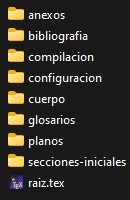
\includegraphics[scale=1]{cuerpo/cap-directorio/imagenes/directorio-raiz}
		\caption[Directorio raíz.]{Directorio raíz. Carpetas que contiene el directorio raíz del archivo \textit{raiz.tex}, que conforma el archivo .tex raíz del documento.}
		\label{subfig:directorio-raiz}
	\end{subfigure}
%	\vfill
	\begin{subfigure}[b]{1\textwidth}
		\centering
		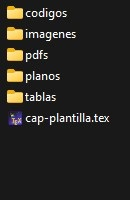
\includegraphics[scale=1]{cuerpo/cap-directorio/imagenes/sub.directorio}
		\caption[Sub-directorio para capítulo.]{Sub-directorio para capítulo. Carpetas para organizar los archivos correspondientes.}
		\label{subfig:directorio-cap}
	\end{subfigure}
	\caption{Estructura del directorio de la plantilla.}
	\label{fig:directorios}
\end{figure}
%
\begin{figure}[h]
	\centering
	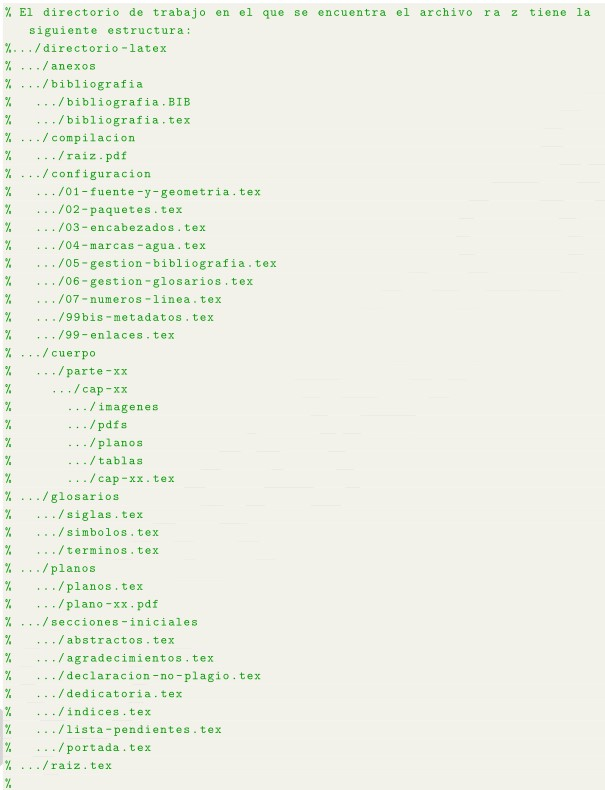
\includegraphics[scale=1, frame]{cuerpo/cap-directorio/imagenes/directorio-raiz-completo}
	\caption[Directorio raíz completo.]{Directorio raíz completo.}
	\label{fig:directorio-raiz-completo}
\end{figure}
%
\part{Formato y Redacción}
\chapter{Formatos}
%
\section{Fuente}
La fuente se elige mediante el archivo \textit{01-fuente-y-geometria.tex}, cargando el paquete específico de la fuente deseada; se configuran en las líneas mostradas en la figura \ref{fig:fuente}.
	\begin{figure}[H]
		\centering
		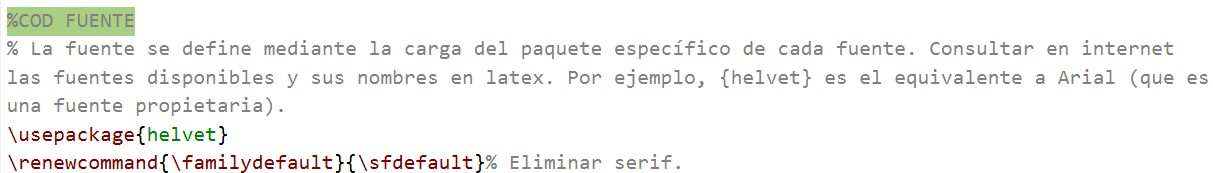
\includegraphics[width=1\linewidth, frame]{cuerpo/cap-redaccion/imagenes/fuente}
		\caption[Tipo de fuente.]{Tipo de fuente. Archivo: .../01-fuente-y-geometria.tex. Por defecto la plantilla usa \textit{helvetic} sin serif.}
		\label{fig:fuente}
	\end{figure}
%
\section{Tamaño de fuente y página}
Se configuran en el archivo raíz del \LaTeX{} (\textit{.../raiz.tex}), según la imagen \ref{fig:fuente-tamano}.
\begin{figure}[H]
	\centering
	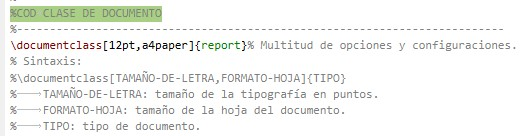
\includegraphics[width=1\linewidth, frame]{cuerpo/cap-redaccion/imagenes/fuente-tamano}
	\caption[Tamaño de letra y página.]{Tamaño de letra y página. Archivo: .../raíz.tex.}
	\label{fig:fuente-tamano}
\end{figure}
%
\subsection{Páginas a una o dos caras}
Se configura en el comando anterior (\ref{fig:fuente-tamano}).
%
\section{Márgenes, interlineado y otros espaciados.}
Se modifican mediante el archivo \textit{01-fuente-y-geometria.tex}, en las líneas mostradas en la figura \ref{fig:margenes-interlineado}.
\begin{figure}[H]
	\centering
	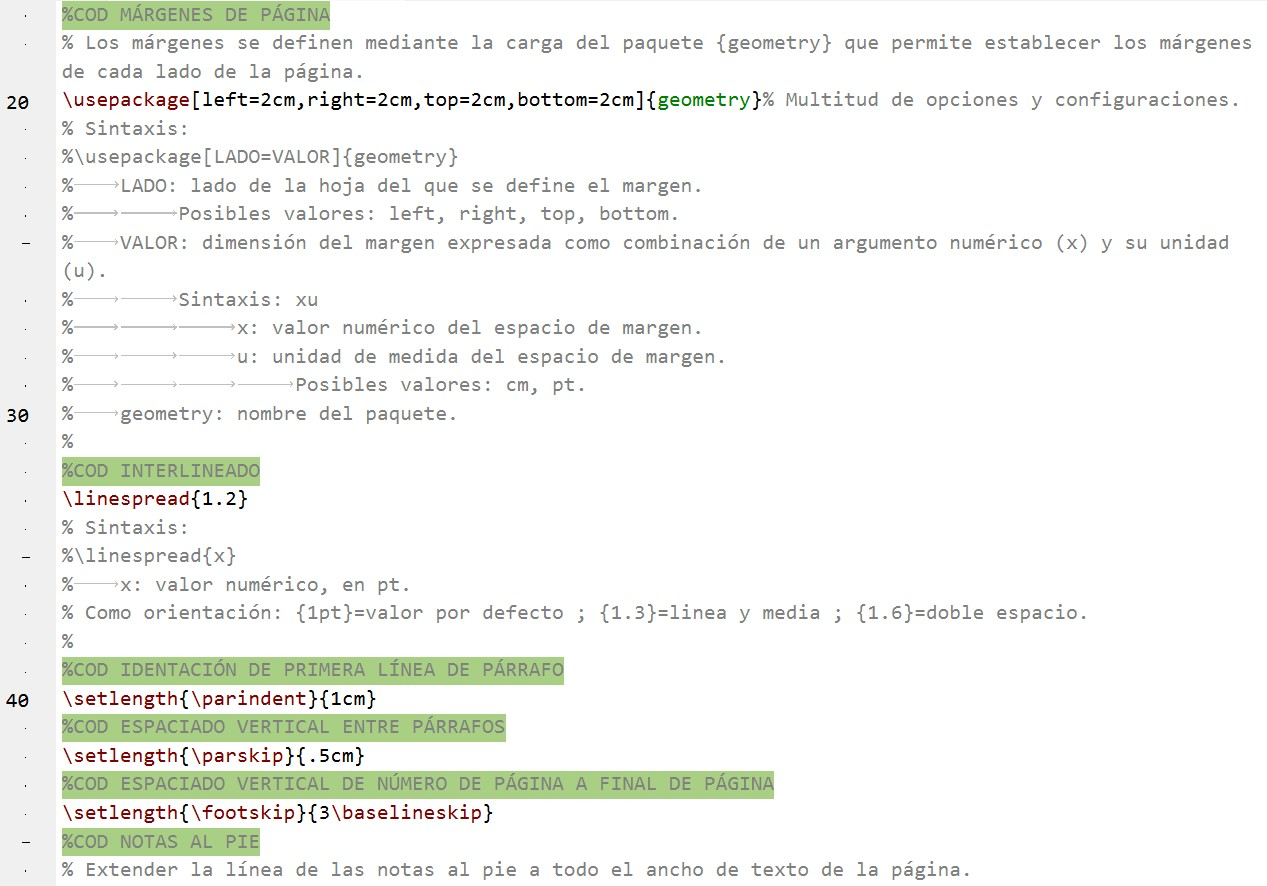
\includegraphics[width=1\linewidth, frame]{cuerpo/cap-redaccion/imagenes/margenes-interlineado}
	\caption[Márgenes e interlineado.]{Márgenes e interlineado. Archivo: .../01-fuente-y-geometria.tex.}
	\label{fig:margenes-interlineado}
\end{figure}
%
\section{Encabezados y pie de página}
Se emplea el paquete \href{https://www.ctan.org/pkg/fancyhdr}{\textit{fancyhdr}}. La configuración se implementa en el archivo .../03-encabezados.tex.
%
\section{Colores}
%
\subsection{Color de la fuente}
%
\subsubsection{Con \textit{\textbackslash color}}
Sintaxis: \textit{\textbackslash color\{COLOR\}}.

Establece el color para todo el texto a partir de ser declarado; para volver al color negro debe declararse explícitamente de nuevo con \textit{black} como argumento.
%
\subsubsection{Con \textit{\textbackslash textcolor}}
Sintaxis: \textit{\textbackslash textcolor\{COLOR\}\{TEXTO\}}.

Modifica solo el texto que se indica en el comando.
%
\subsection{Resalte de texto}
Sintaxis: \textbackslash \textit{hlc[COLOR]\{TEXTO\}}.

Modifica solo el texto que se indica en el comando.
%
\subsection{Ejemplos de cambios de color}
Esta linea debiera ser en color negro estándar.

\color{red}
Este linea debiera ser en color rojo.

Esta linea debiera ser en color negro estándar; pero es roja porque sigue activo el comando \textbackslash \textit{color\{red\}} que se declaró para la linea anterior.

\textcolor{green}{Esta linea debiera ser verde; porque se ha escrito dentro de un comando \textbackslash \textit{textcolor\{green\}}.}

Esta linea debiera ser en color negro estándar; pero es roja porque sigue activo el comando \textbackslash \textit{color\{red\}} que se declaró para la primera linea roja.

\color{brown}
Esta linea es marrón porque se ha declarado un \textbackslash \textit{color\{brown\}}.

\textcolor{purple}{Esta linea es púrpura; porque se ha escrito dentro de un comando \textbackslash \textit{textcolor\{purple\}}.}

\hlc[orange]{Esta linea tiene fuente marrón por el comando \textbackslash \textit{color\{brown\}} anterior; está resaltada en naranja por haber aplicado un comando \textbackslash \textit{hlc[orange]}}

\color{black}
Esta linea es negra porque se ha declarado un \textbackslash \textit{color\{black\}}.

\hlc[cyan]{Esta linea tiene fuente negra por haber restablecido el negro en la linea anterior; está resaltada en cian por haber aplicado un comando \textbackslash \textit{hlc[cyan]}.}

El código empleado es el mostrado en la figura \ref{fig:colores-codigo}.
\begin{figure}[h]
	\centering
	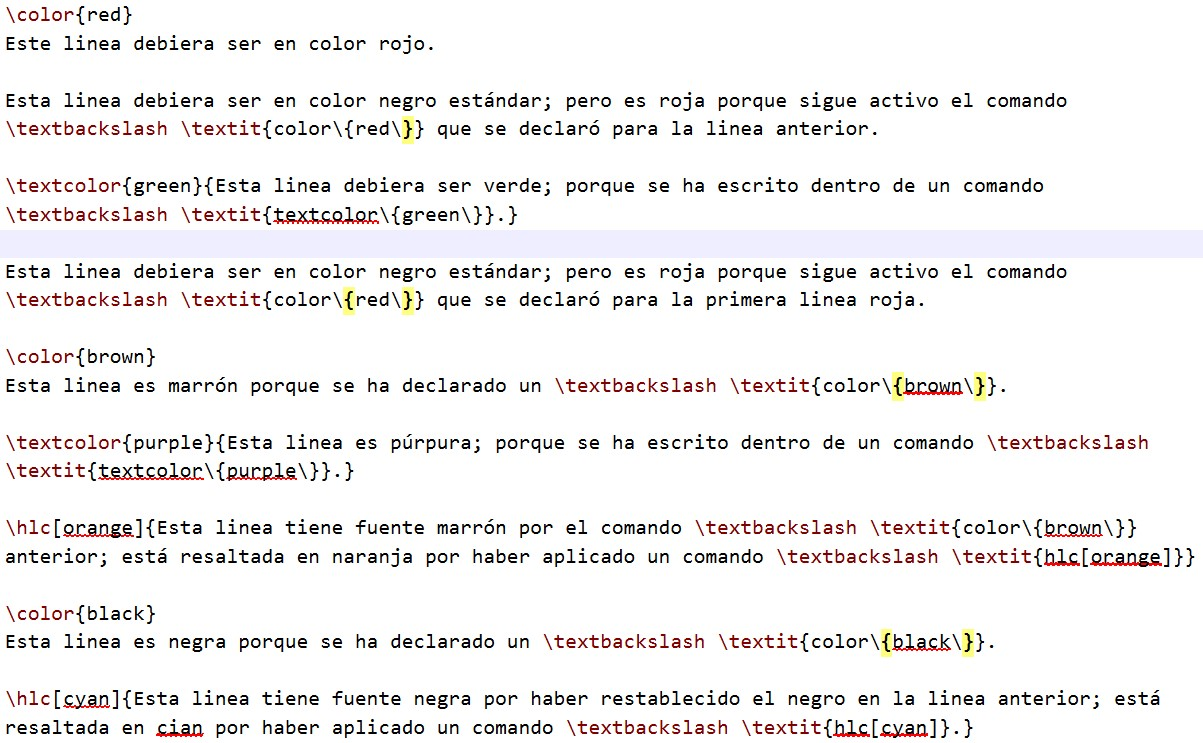
\includegraphics[width=1\linewidth, frame]{cuerpo/cap-redaccion/imagenes/colores-codigo}
	\caption[Colores y resalte de texto.]{Colores y resalte de texto.}
	\label{fig:colores-codigo}
\end{figure}
%
\subsection{Color de enlaces}
Es una configuración para todo el \LaTeX{} que se define en el archivo \textit{.../99-enlaces.tex}, como parte del paquete \href{https://www.ctan.org/pkg/hyperref}{\textit{hyperref}}, según se muestra en la imagen \ref{fig:color-enlaces}.
\begin{figure}[H]
	\centering
	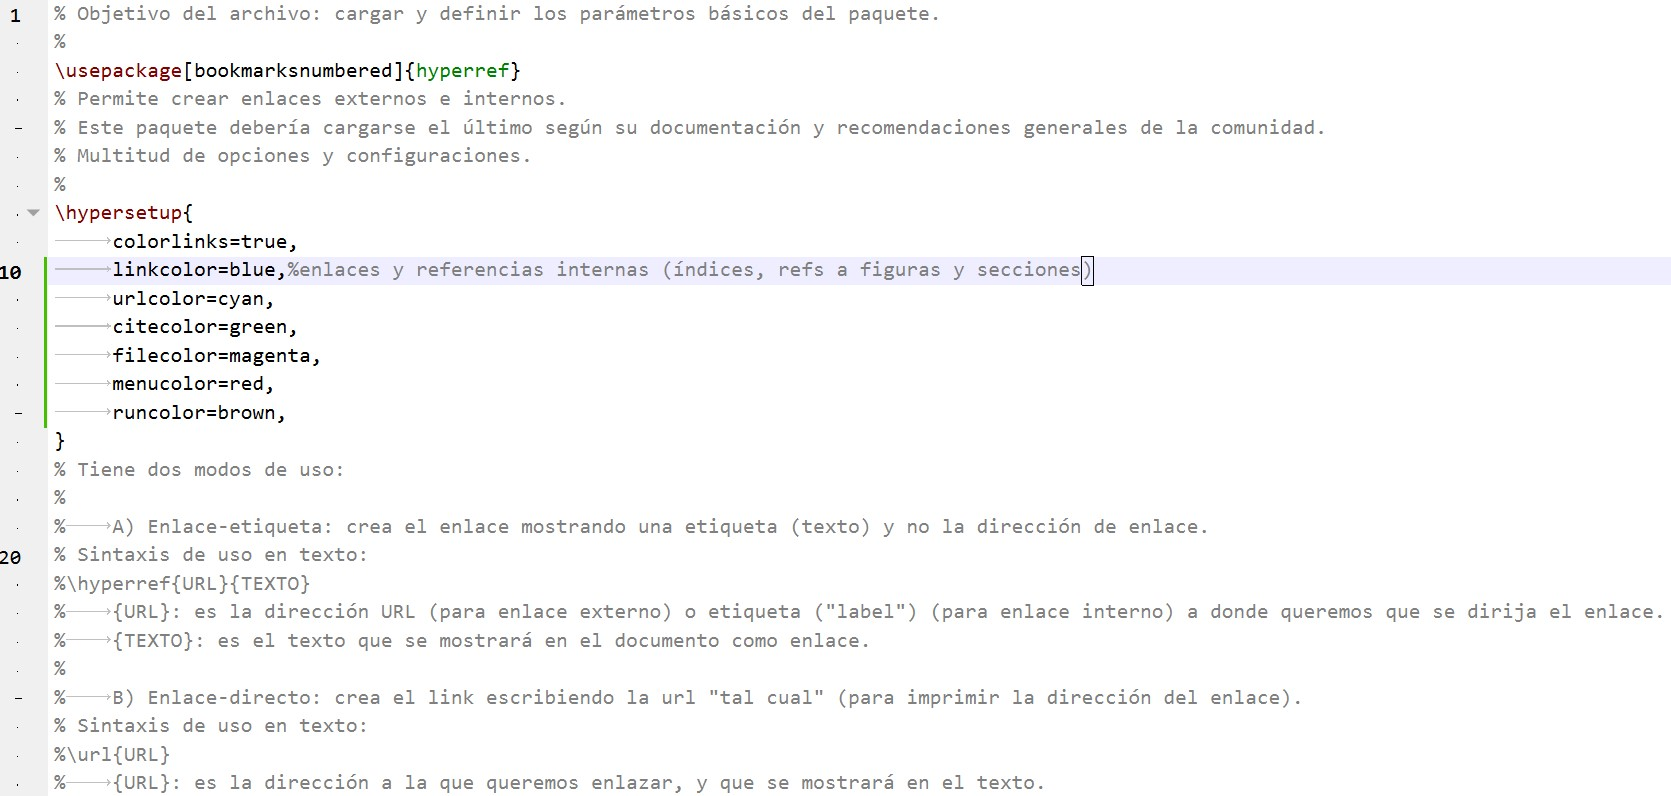
\includegraphics[width=1\linewidth, frame]{cuerpo/cap-redaccion/imagenes/color-enlaces}
	\caption[Color de enlaces.]{Color de enlaces. Archivo: .../99-enlaces.tex.}
	\label{fig:color-enlaces}
\end{figure}
%
\subsection{Color de la página}
Sintaxis: \textit{\textbackslash pagecolor\{COLOR\}}.

Establece el color a partir de ser insertado para el resto del documento, para volver al color blanco debe declararse explícitamente con \textbackslash\textit{nopagecolor}.
%
\part{Uso y gestión de objetos}
\chapter{Imágenes}
%
\section{Insertar imagen}
Para incluir imágenes se puede usar el asistente de TeXstudio cuya interfaz es la mostrada en la figura \ref{fig:auxiliar-imagenes}.

\begin{figure}[h]
	\centering
	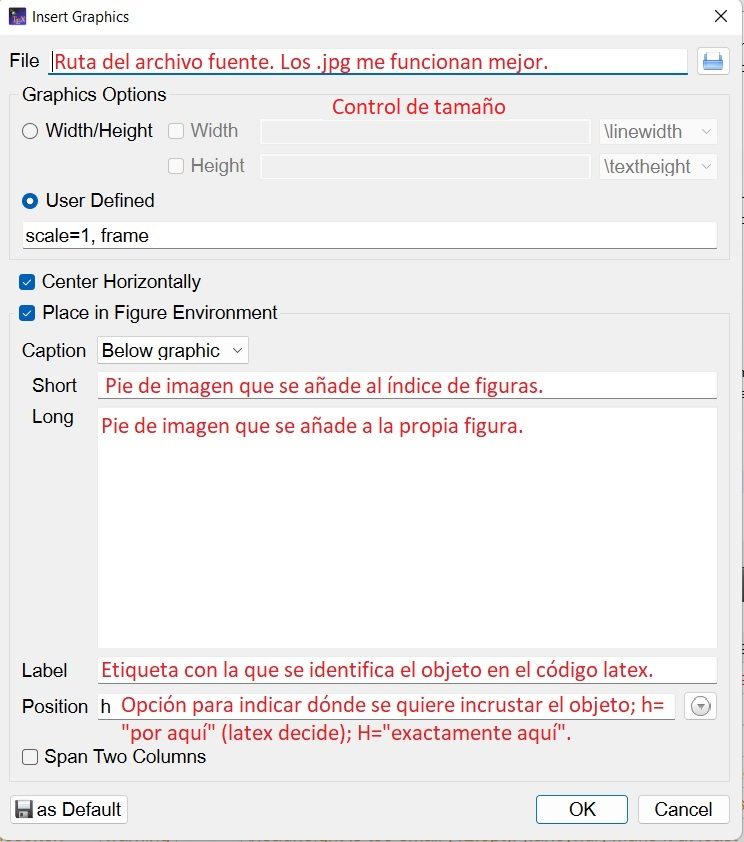
\includegraphics[scale=.65, frame]{cuerpo/cap-objetos/imagenes/auxiliar-imagenes}
	\caption[Interfaz del asistente de imágenes de TeXstudio.]{Interfaz del asistente de imágenes de TeXstudio. En rojo notas sobre algunos campos que permiten personalizar la imagen.}
	\label{fig:auxiliar-imagenes}
\end{figure}
%
\section{Pie de figura}
La configuración del pie de la figura se realiza en el archivo de configuración \textit{02-paquetes.tex}, en las líneas que se muestran en la figura \ref{fig:personalizacion-pies}. Se emplea el paquete \href{https://www.ctan.org/pkg/caption}{\textit{caption}}.

\begin{figure}[h]
	\centering
	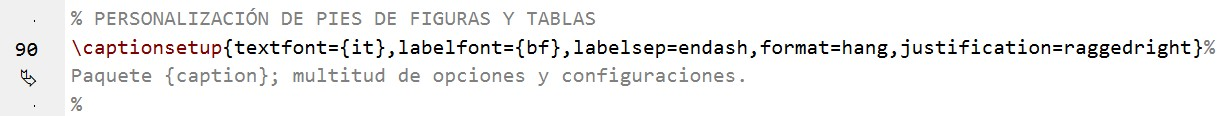
\includegraphics[width=1\textwidth, frame]{cuerpo/cap-objetos/imagenes/personalizacion-pies}
	\caption[Configuración de pies de objetos.]{Configuración de pies de objetos. El comando mostrado se emplea para configurar los pies de los objetos tipo \textit{caption}, que incluye figuras, tablas, código importado. Archivo: .../raiz/configuracion/02-paquetes.tex}.
	\label{fig:personalizacion-pies}
\end{figure}
%
\newpage
Se incluyen a continuación ejemplos de disposiciones frecuentes de imágenes; el código empelado es el mostrado en el fragmento \ref{cod-fig-ejemplo}.
\lstinputlisting[frame={single}, language={[AlLaTeX]TeX}, label={cod-fig-ejemplo}, caption=Código para las imágenes ejemplo \ref{fig:robotdevil} a \ref{fig:grafico-multiple}]{cuerpo/cap-objetos/codigos/imagenes-01.txt}.
%
\begin{figure}[H]
	\centering
	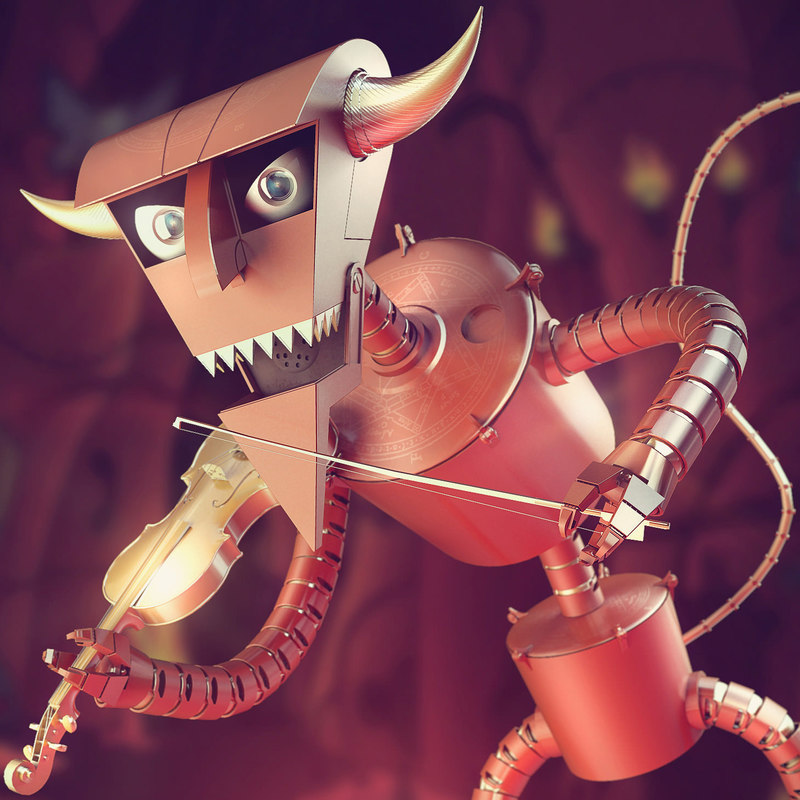
\includegraphics[scale=1.5, frame]{cuerpo/cap-objetos/imagenes/robotdevil.jpg}
	\caption[Imagen simple 1.]{Imagen simple 1. Una única imagen.}
	\label{fig:robotdevil}
\end{figure}
%
\begin{figure}[H]
	\centering
	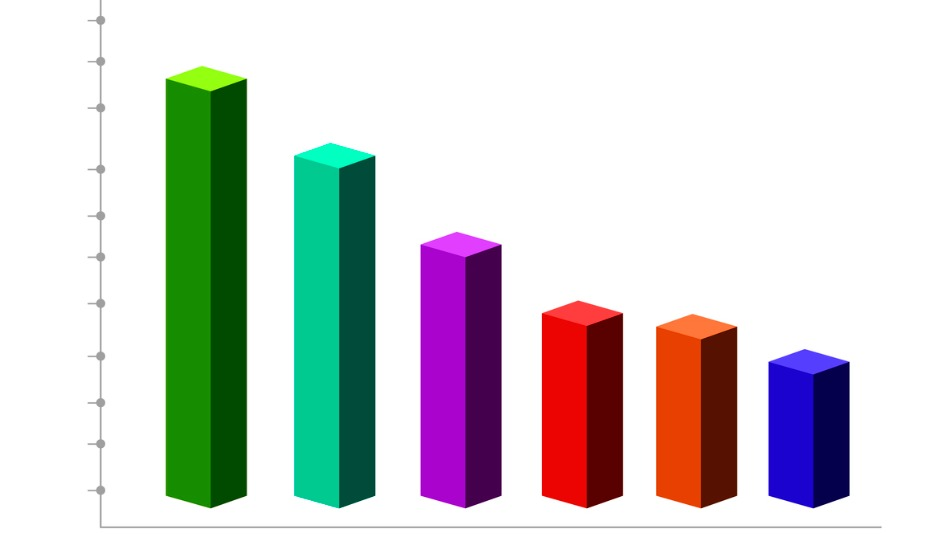
\includegraphics[scale=.5]{cuerpo/cap-objetos/imagenes/grafico-de-barras}
	\caption[Gráfico simple 1.]{Gráfico simple 1. Un gráfico, con fondo blanco y sin borde en la imagen fuente.}
	\label{fig:grafico-de-barras}
\end{figure}
%
\begin{figure}[H]
	\centering
	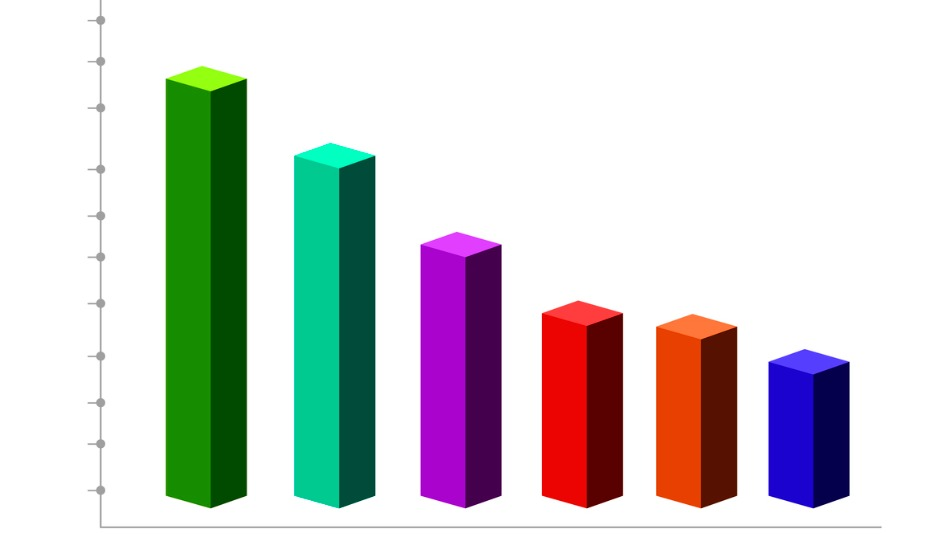
\includegraphics[scale=.5, frame]{cuerpo/cap-objetos/imagenes/grafico-de-barras}
	\caption[Gráfico simple 2.]{Gráfico simple 2. Un gráfico, con fondo blanco y sin borde en la imagen fuente, pero con el borde añadido en \LaTeX; por defecto esta plantilla añade el borde.}
	\label{fig:grafico-de-barras-bis}
\end{figure}
%
\begin{figure}[H]
	\centering
	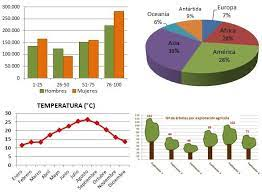
\includegraphics[scale=1, frame]{cuerpo/cap-objetos/imagenes/grafico-multiple}
	\caption[Gráfico simple 3.]{Gráfico simple 3. Un gráfico cuya imagen fuente es un collage de varias imágenes, por lo que en realidad es un único objeto.}
	\label{fig:grafico-multiple}
\end{figure}
%
\section{Subfiguras}
Se pueden crear figuras compuestas de subfiguras.
\begin{figure}[H]
	\centering
	\begin{subfigure}[b]{0.45\textwidth}
		\centering
		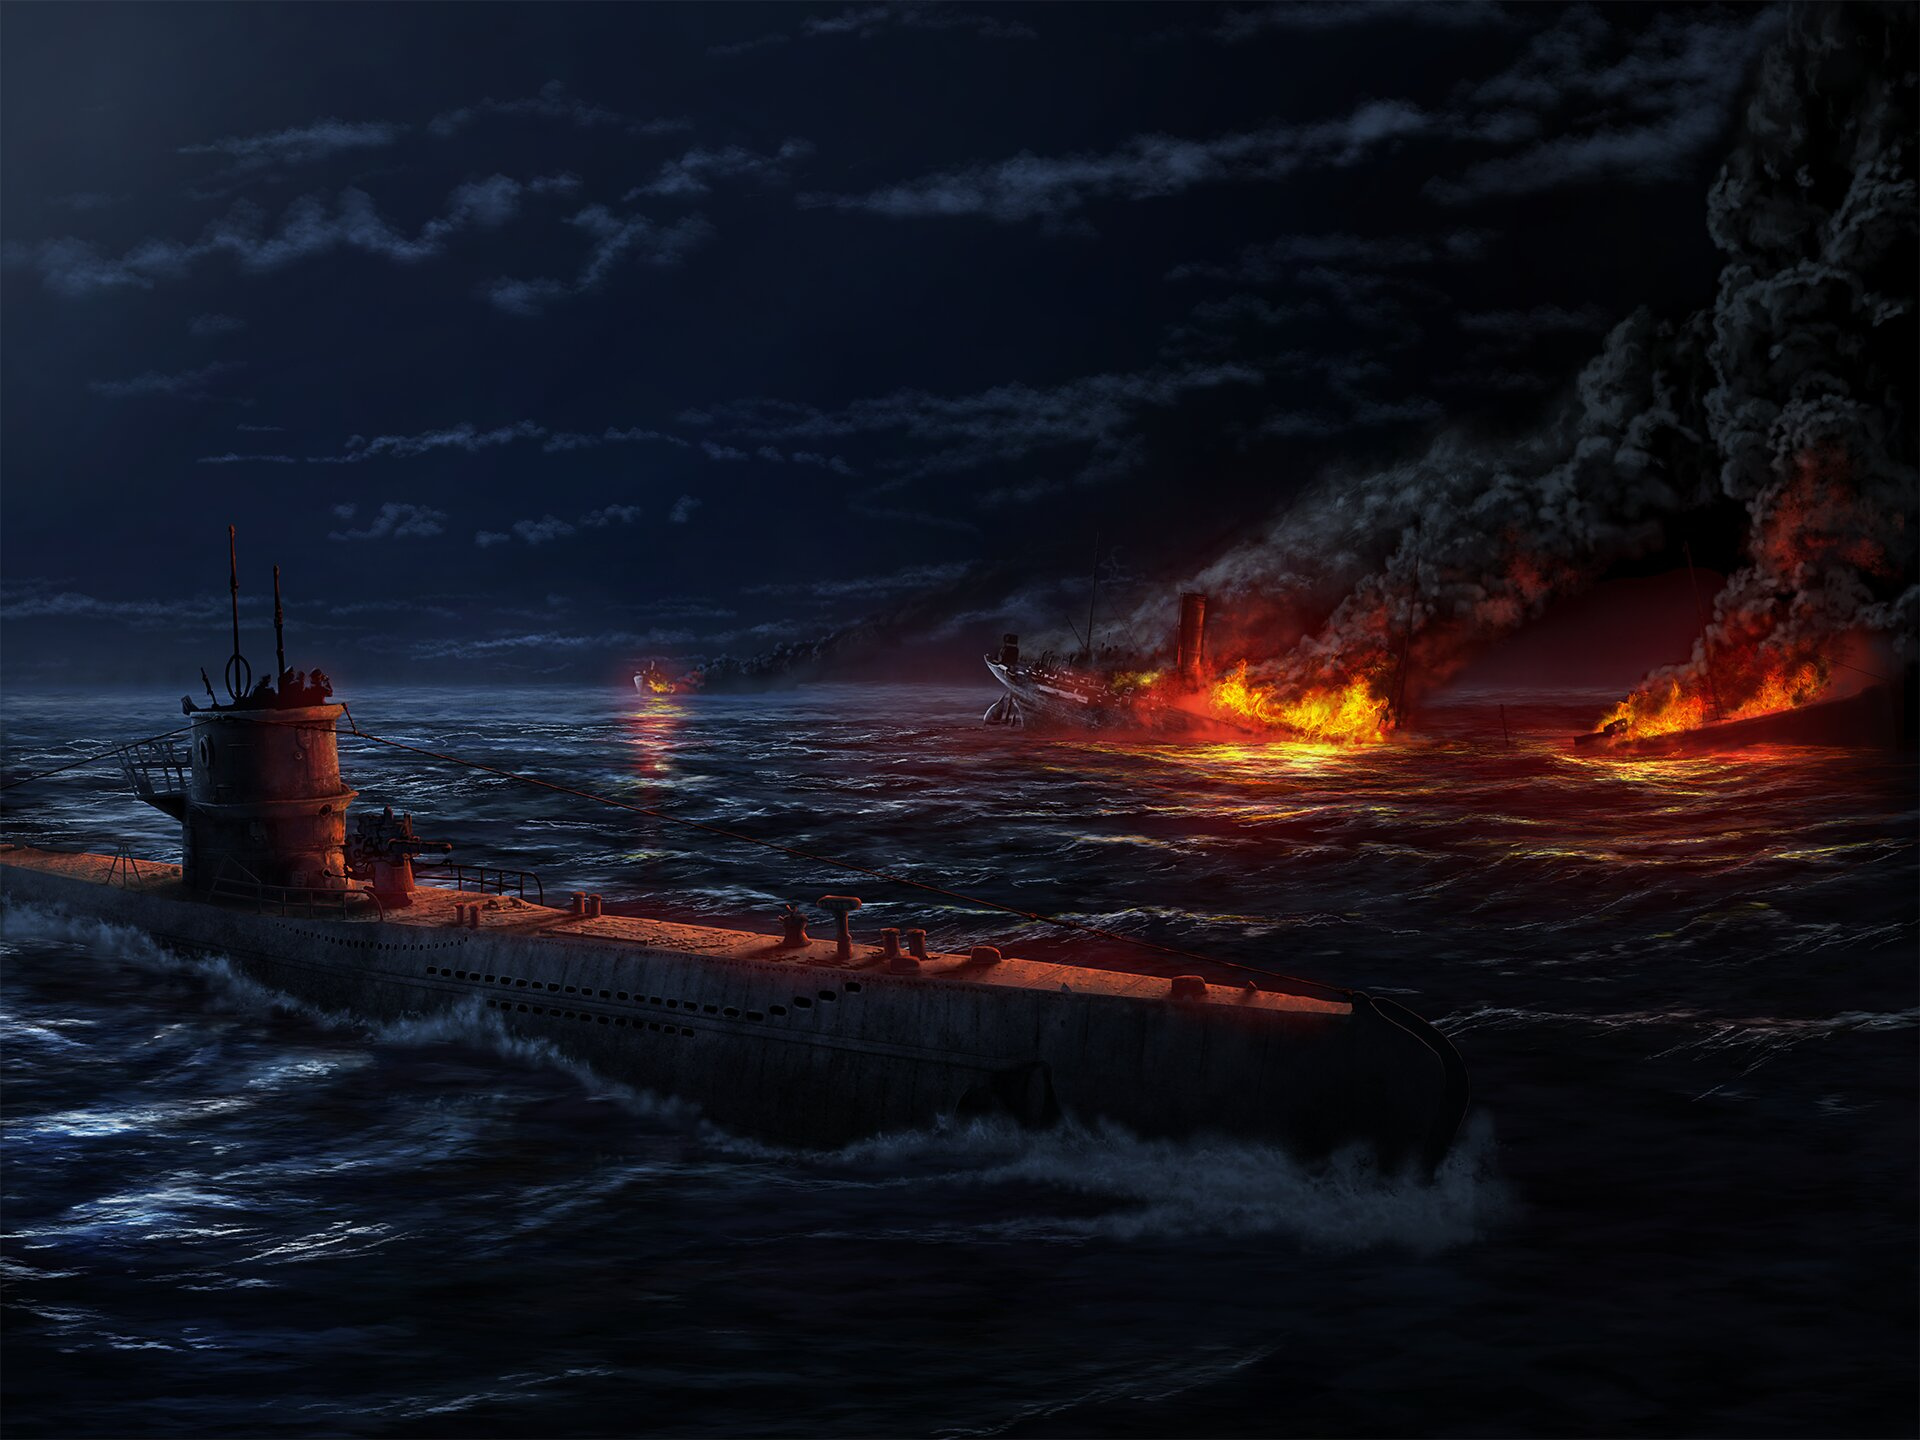
\includegraphics[width=\textwidth]{cuerpo/cap-objetos/imagenes/hoi4-convoy-raiding}
		\caption{Uboat atacando convoy.}
		\label{fig:hoi4-convoy-raiding}
	\end{subfigure}
	%
	\begin{subfigure}[b]{0.45\textwidth}
		\centering
		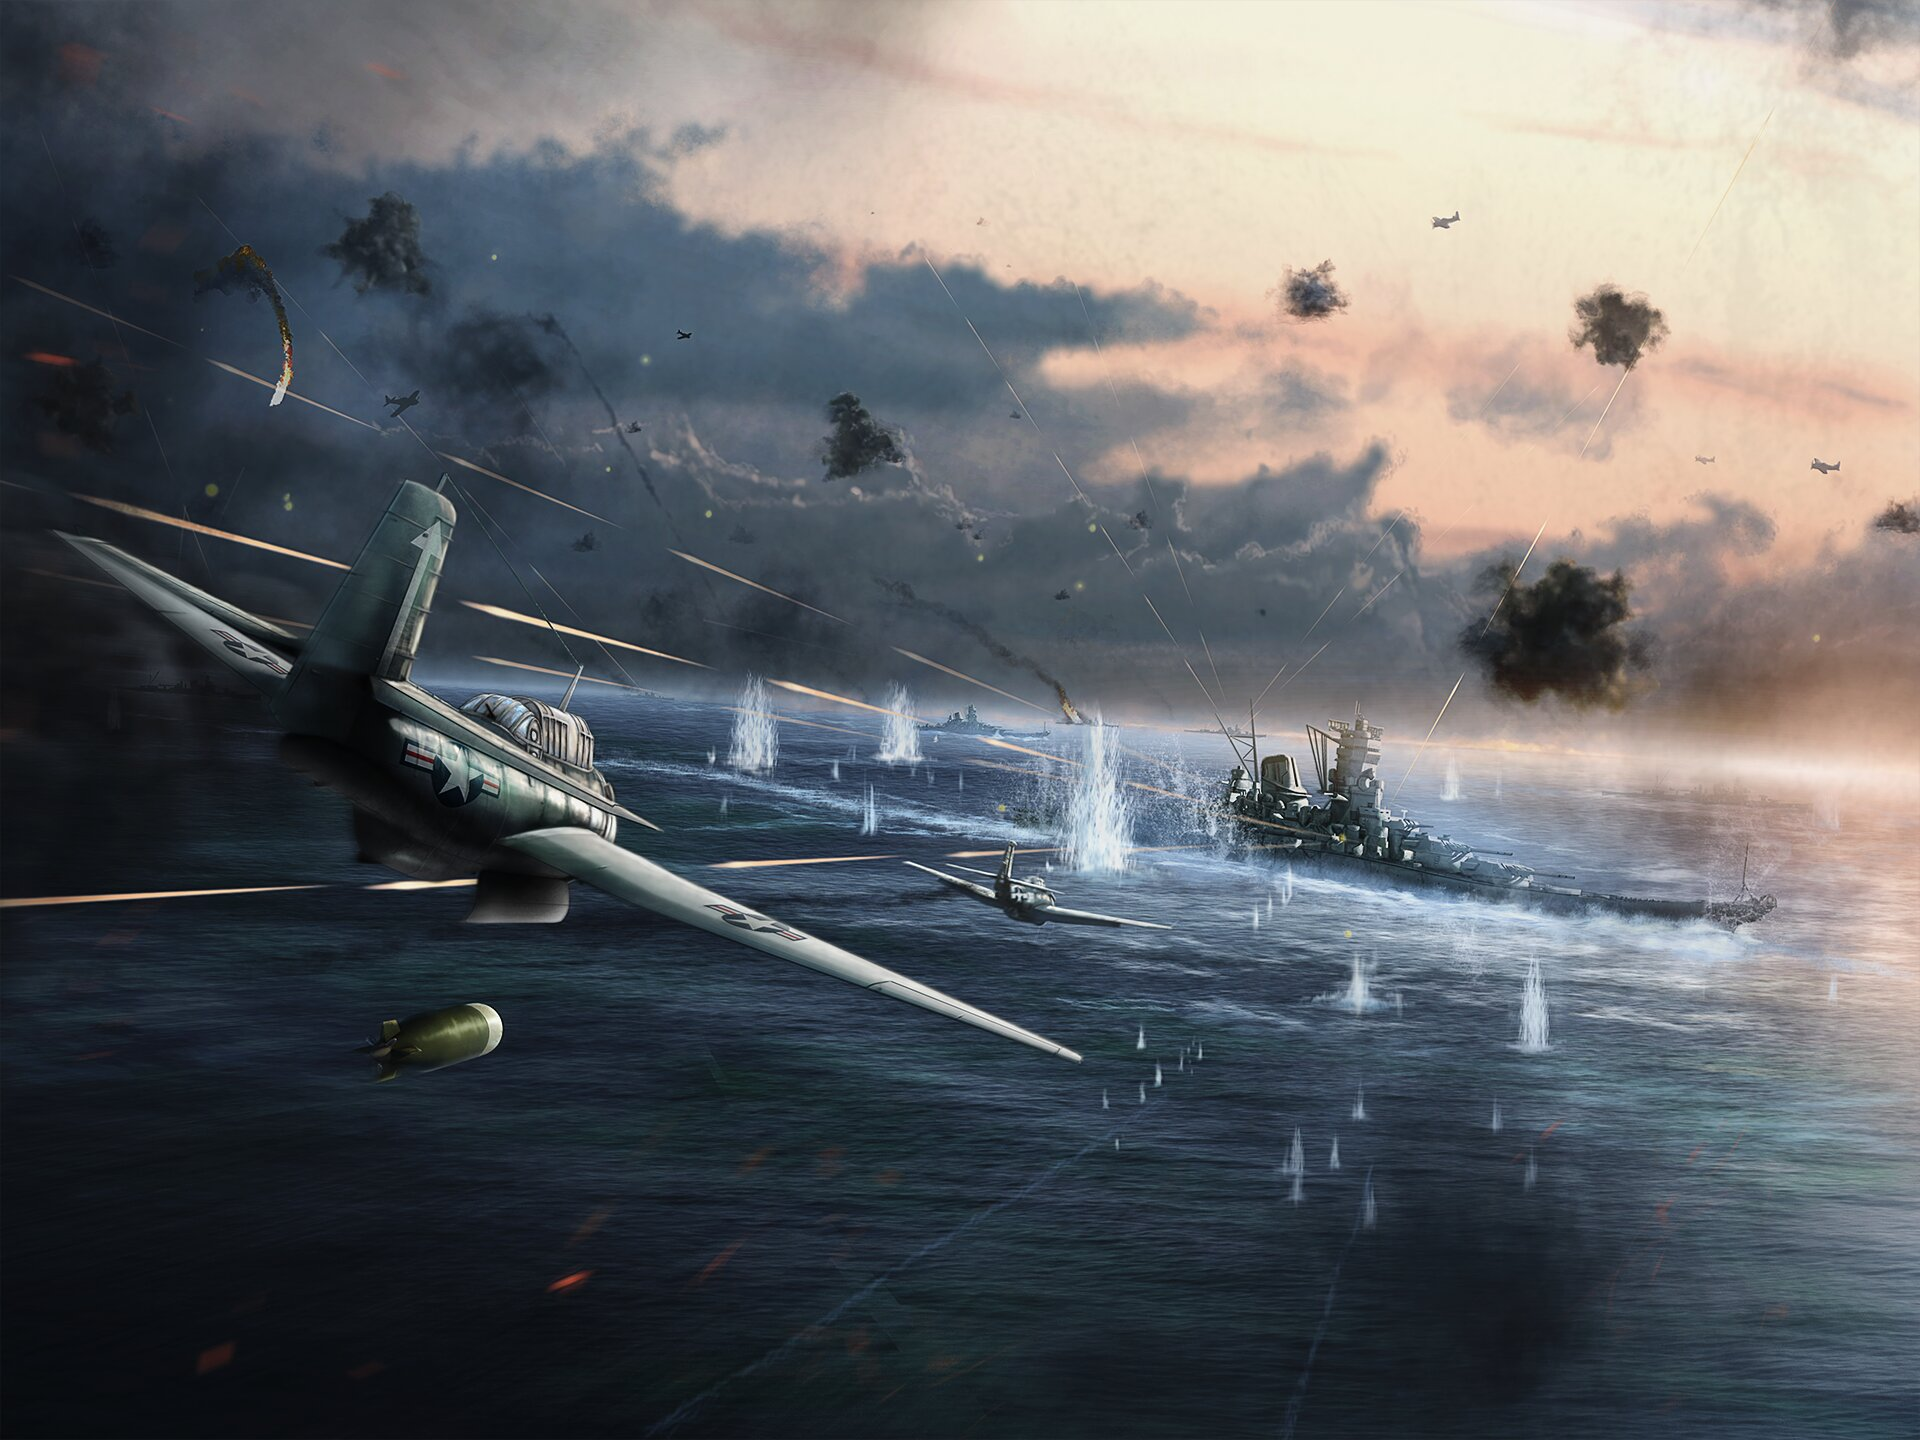
\includegraphics[width=\textwidth]{cuerpo/cap-objetos/imagenes/hoi4-aeronaval-battle}
		\caption{Torpedero naval atacando acorazado.}
		\label{fig:hoi4-aeronaval-battle}
	\end{subfigure}
	\caption[Figura con 2 subfiguras - ejemplo 1.]{Figura con 2 subfiguras - ejemplo 1. Figuras alineadas inferiormente y en una misma linea. Batallas aeronavales de la Segunda Guerra Mundial. Fuente: \cite{hoi4}.}
	\label{fig:aeronavales}
\end{figure}
%
%\newpage
\lstinputlisting[frame={single}, language={[AlLaTeX]TeX}, label={cod-fig:aeronavales}, caption=Código de la figura \ref{fig:aeronavales}.]{cuerpo/cap-objetos/codigos/subfigura1.txt}
%
\begin{figure}[H]
	\centering
	\begin{subfigure}[b]{1\textwidth}
		\centering
		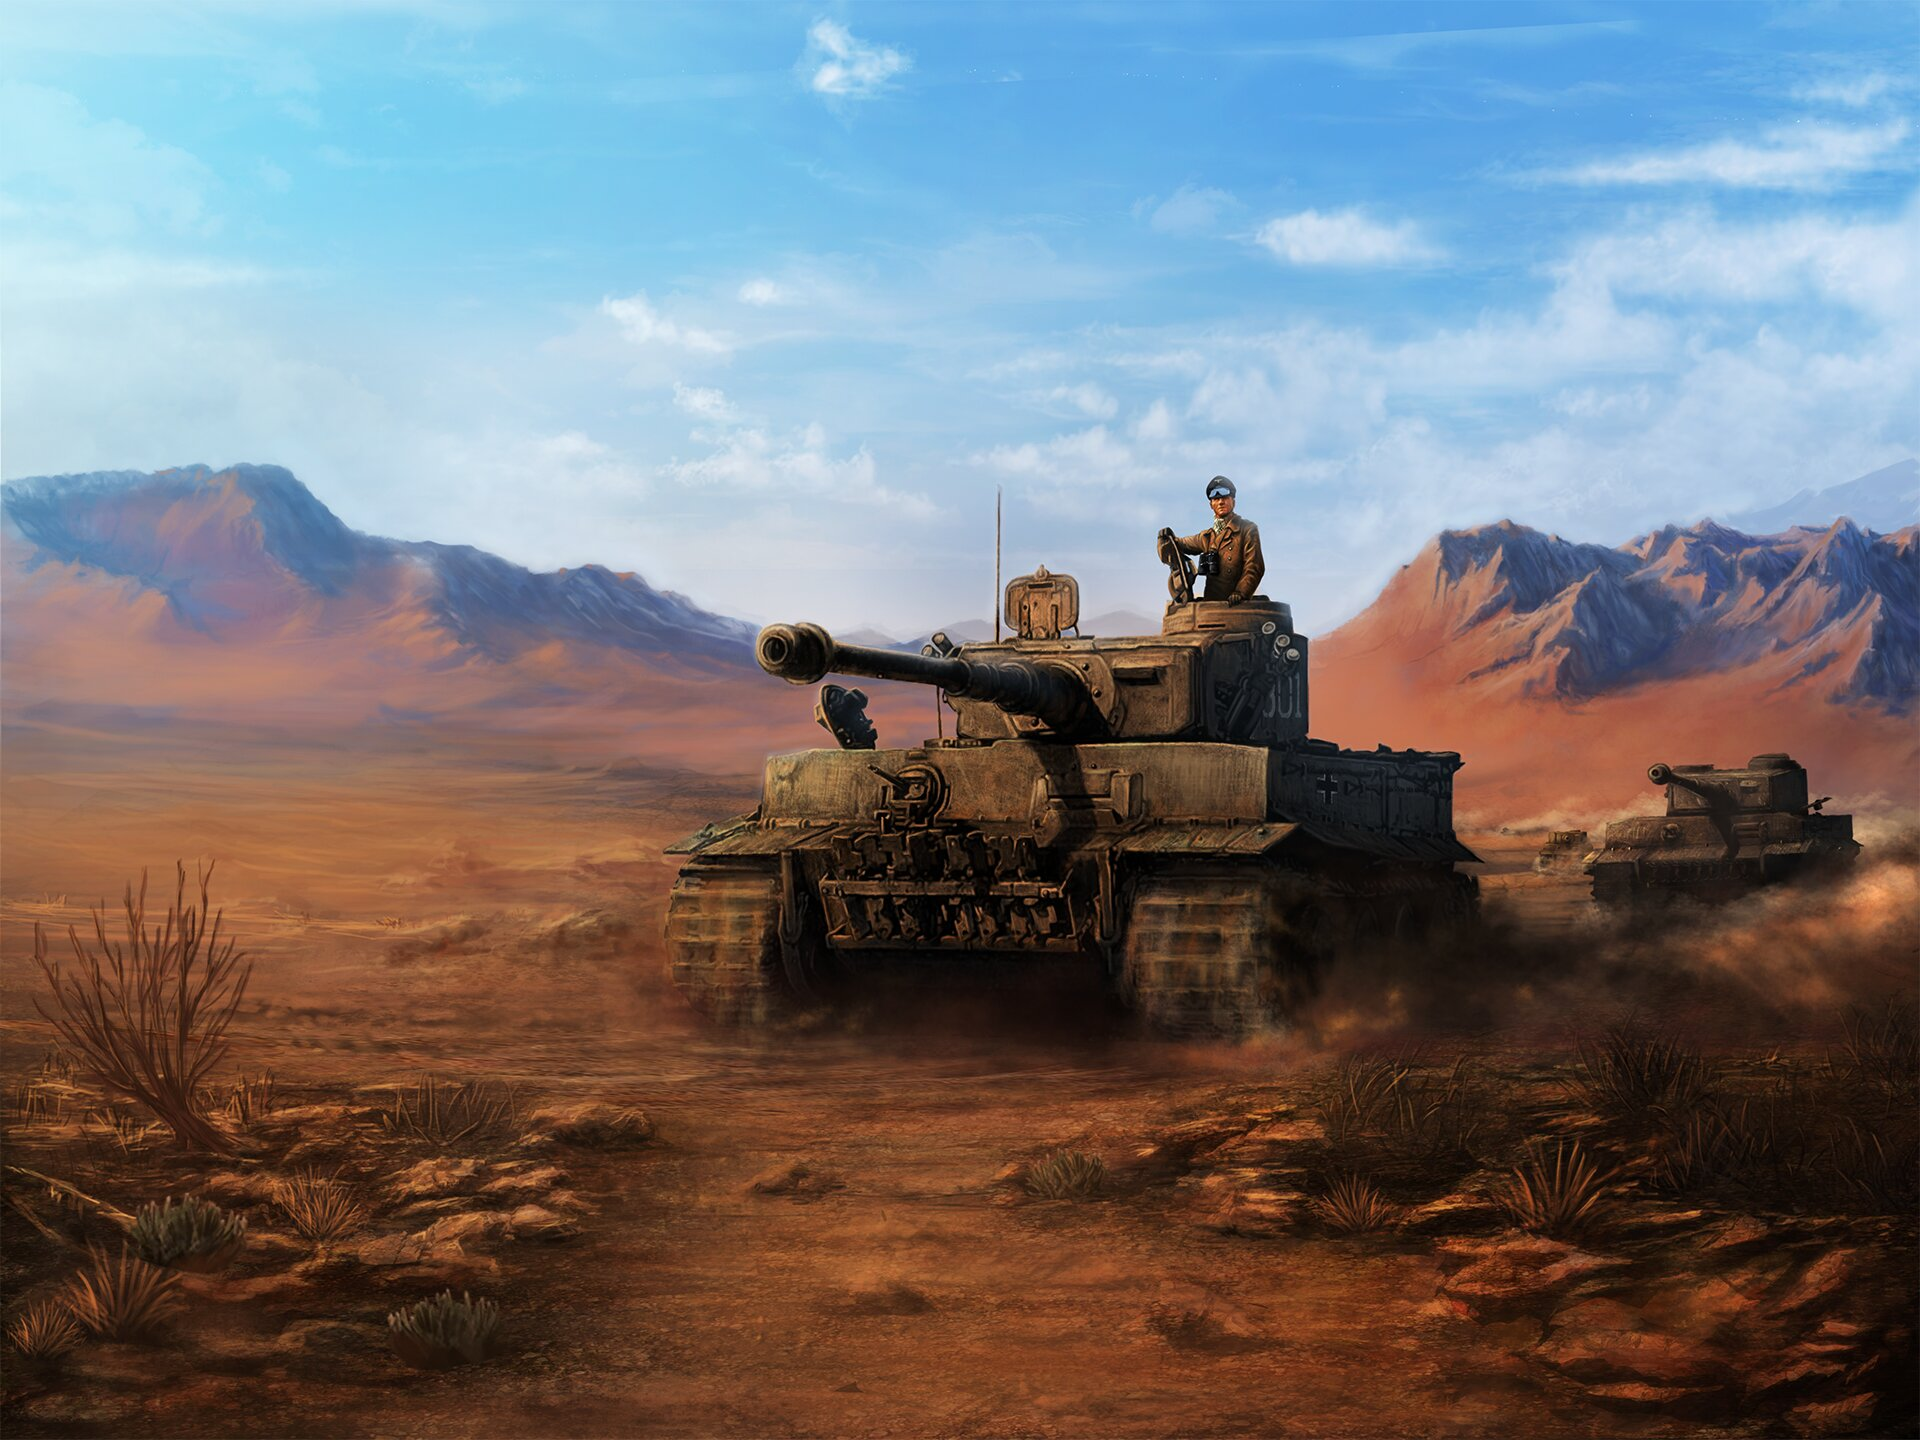
\includegraphics[width=0.75\textwidth]{cuerpo/cap-objetos/imagenes/hoi4-afrika-korps}
		\caption{Afrika korps.}
		\label{fig:hoi4-afrika-korps}
	\end{subfigure}
	%
	\begin{subfigure}[b]{1\textwidth}
		\centering
		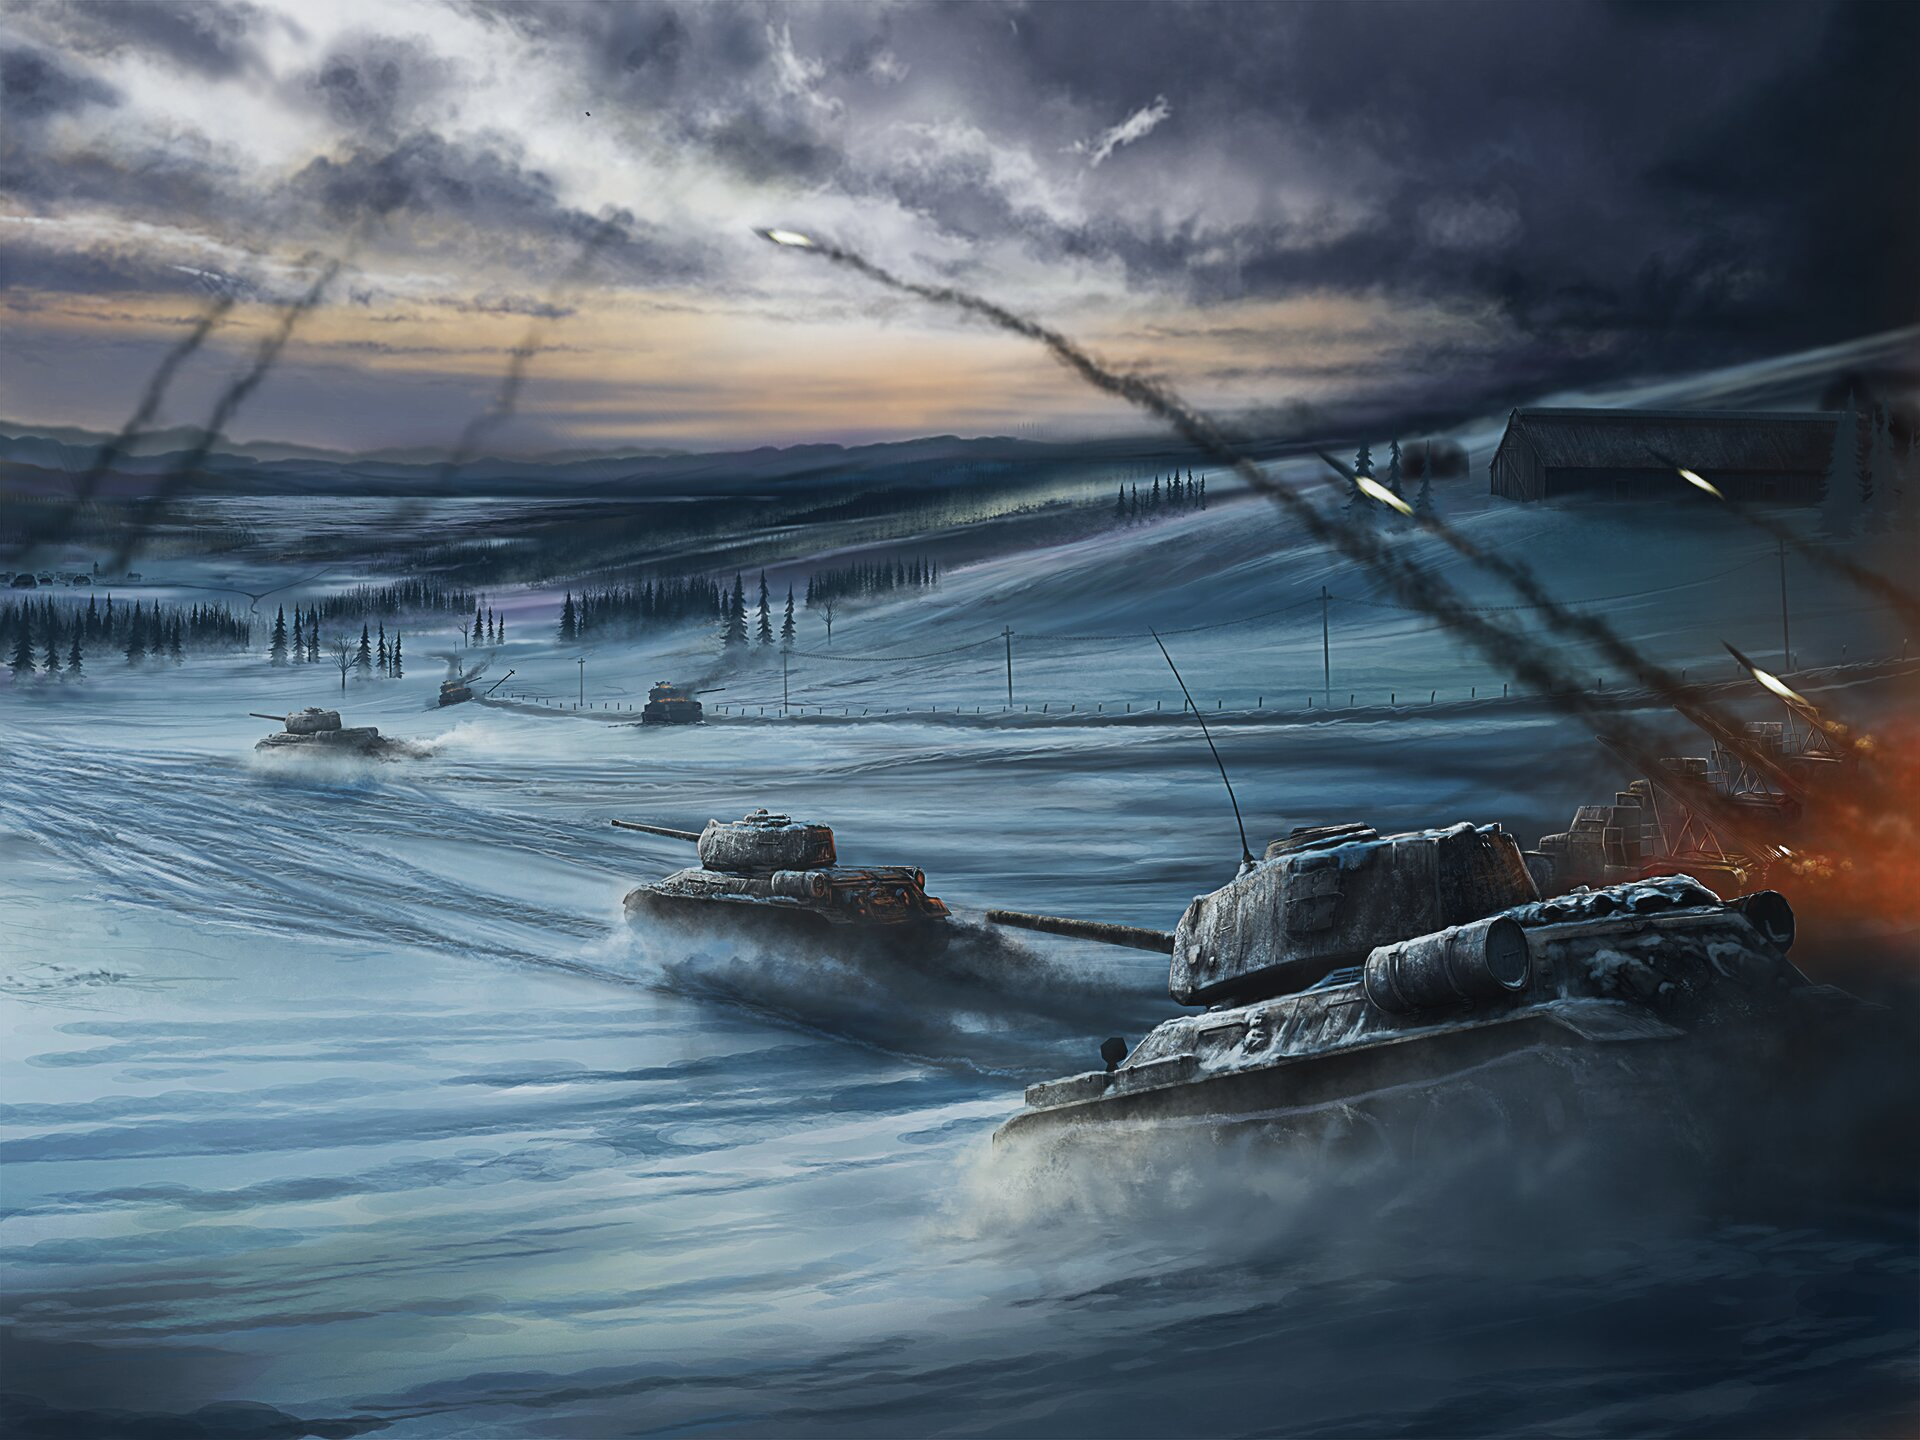
\includegraphics[width=0.75\textwidth]{cuerpo/cap-objetos/imagenes/hoi4-soviet-tanks}
		\caption{Tanques soviéticos.}
		\label{fig:hoi4-soviet-tanks}
	\end{subfigure}
	%
	\caption[Figura con 2 subfiguras - ejemplo 2.]{Figura con 2 subfiguras - ejemplo 2. Figuras alineadas inferiormente y en diferentes lineas. Tanques en la Segunda Guerra Mundial. Fuente: \cite{hoi4}.}
	\label{fig:tanques}
\end{figure}
%
\newpage
\lstinputlisting[frame={single}, language={[AlLaTeX]TeX}, label={cod-fig:tanques}, caption=Código de la figura \ref{fig:tanques}.]{cuerpo/cap-objetos/codigos/subfigura2.txt}
%
\begin{figure}[H]
	\centering
	\begin{subfigure}[b]{0.45\textwidth}
		\centering
		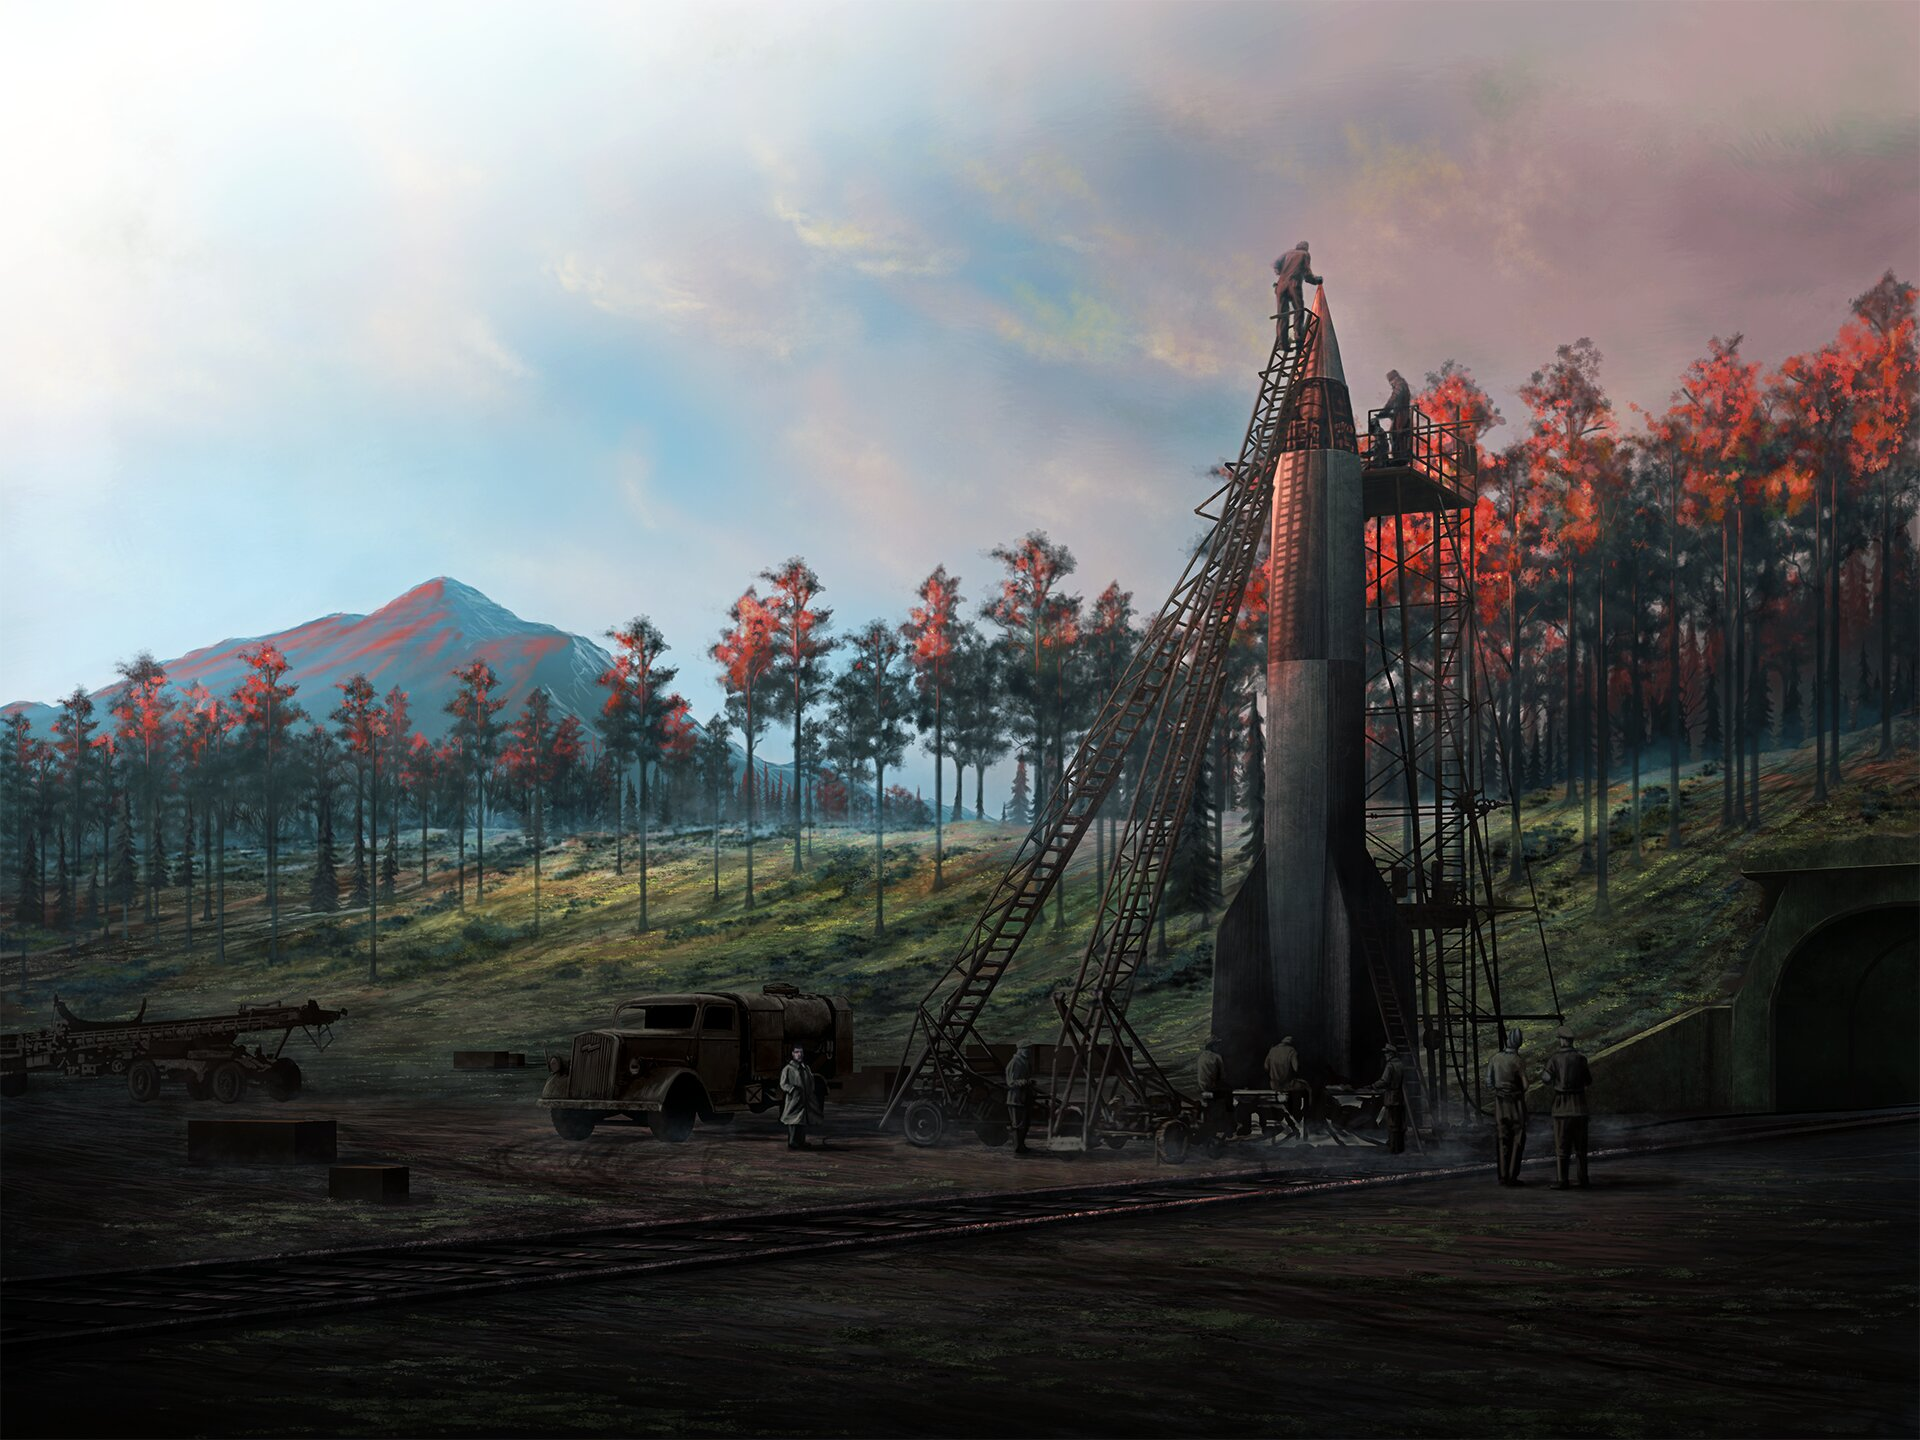
\includegraphics[width=\textwidth, frame]{cuerpo/cap-objetos/imagenes/hoi4-v2}
		\caption{V2.}
		\label{fig:hoi4-v2}
	\end{subfigure}
	%
	\begin{subfigure}[b]{0.45\textwidth}
		\centering
		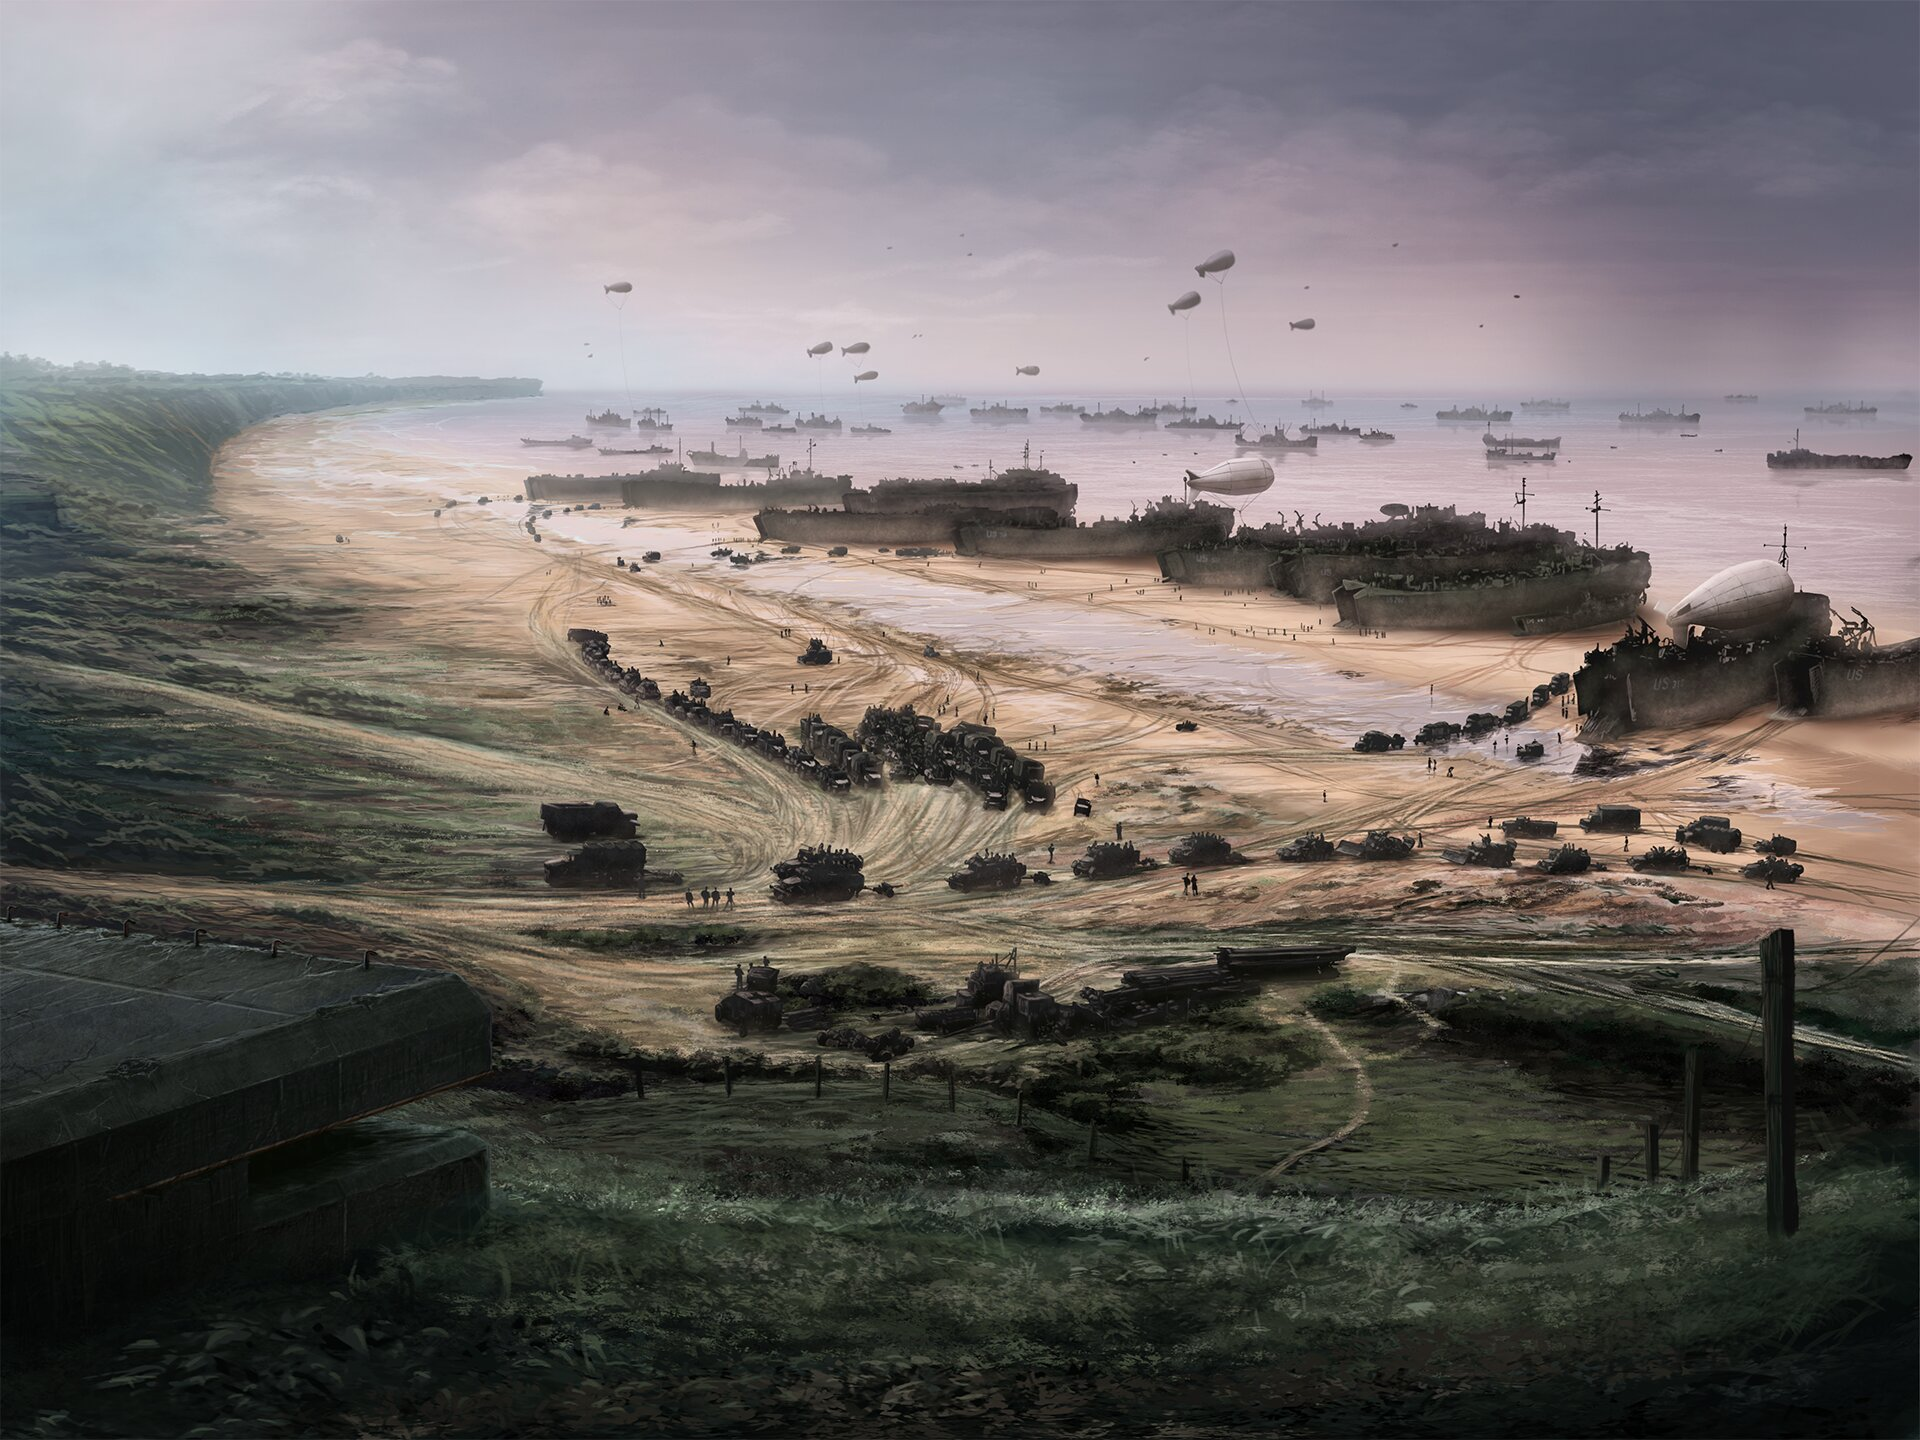
\includegraphics[width=\textwidth, frame]{cuerpo/cap-objetos/imagenes/hoi4-normandy-landing}
		\caption{Desembarco en Normandía.}
		\label{fig:hoi4-normandia}
	\end{subfigure}
	\hfill
		\begin{subfigure}[b]{0.45\textwidth}
		\centering
		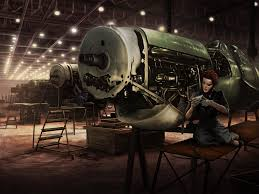
\includegraphics[width=\textwidth, frame]{cuerpo/cap-objetos/imagenes/hoi4-female-worker}
		\caption{Mujer en fábrica de armamento.}
		\label{fig:hoi4-female-worker}
	\end{subfigure}
	%
	\begin{subfigure}[b]{0.45\textwidth}
		\centering
		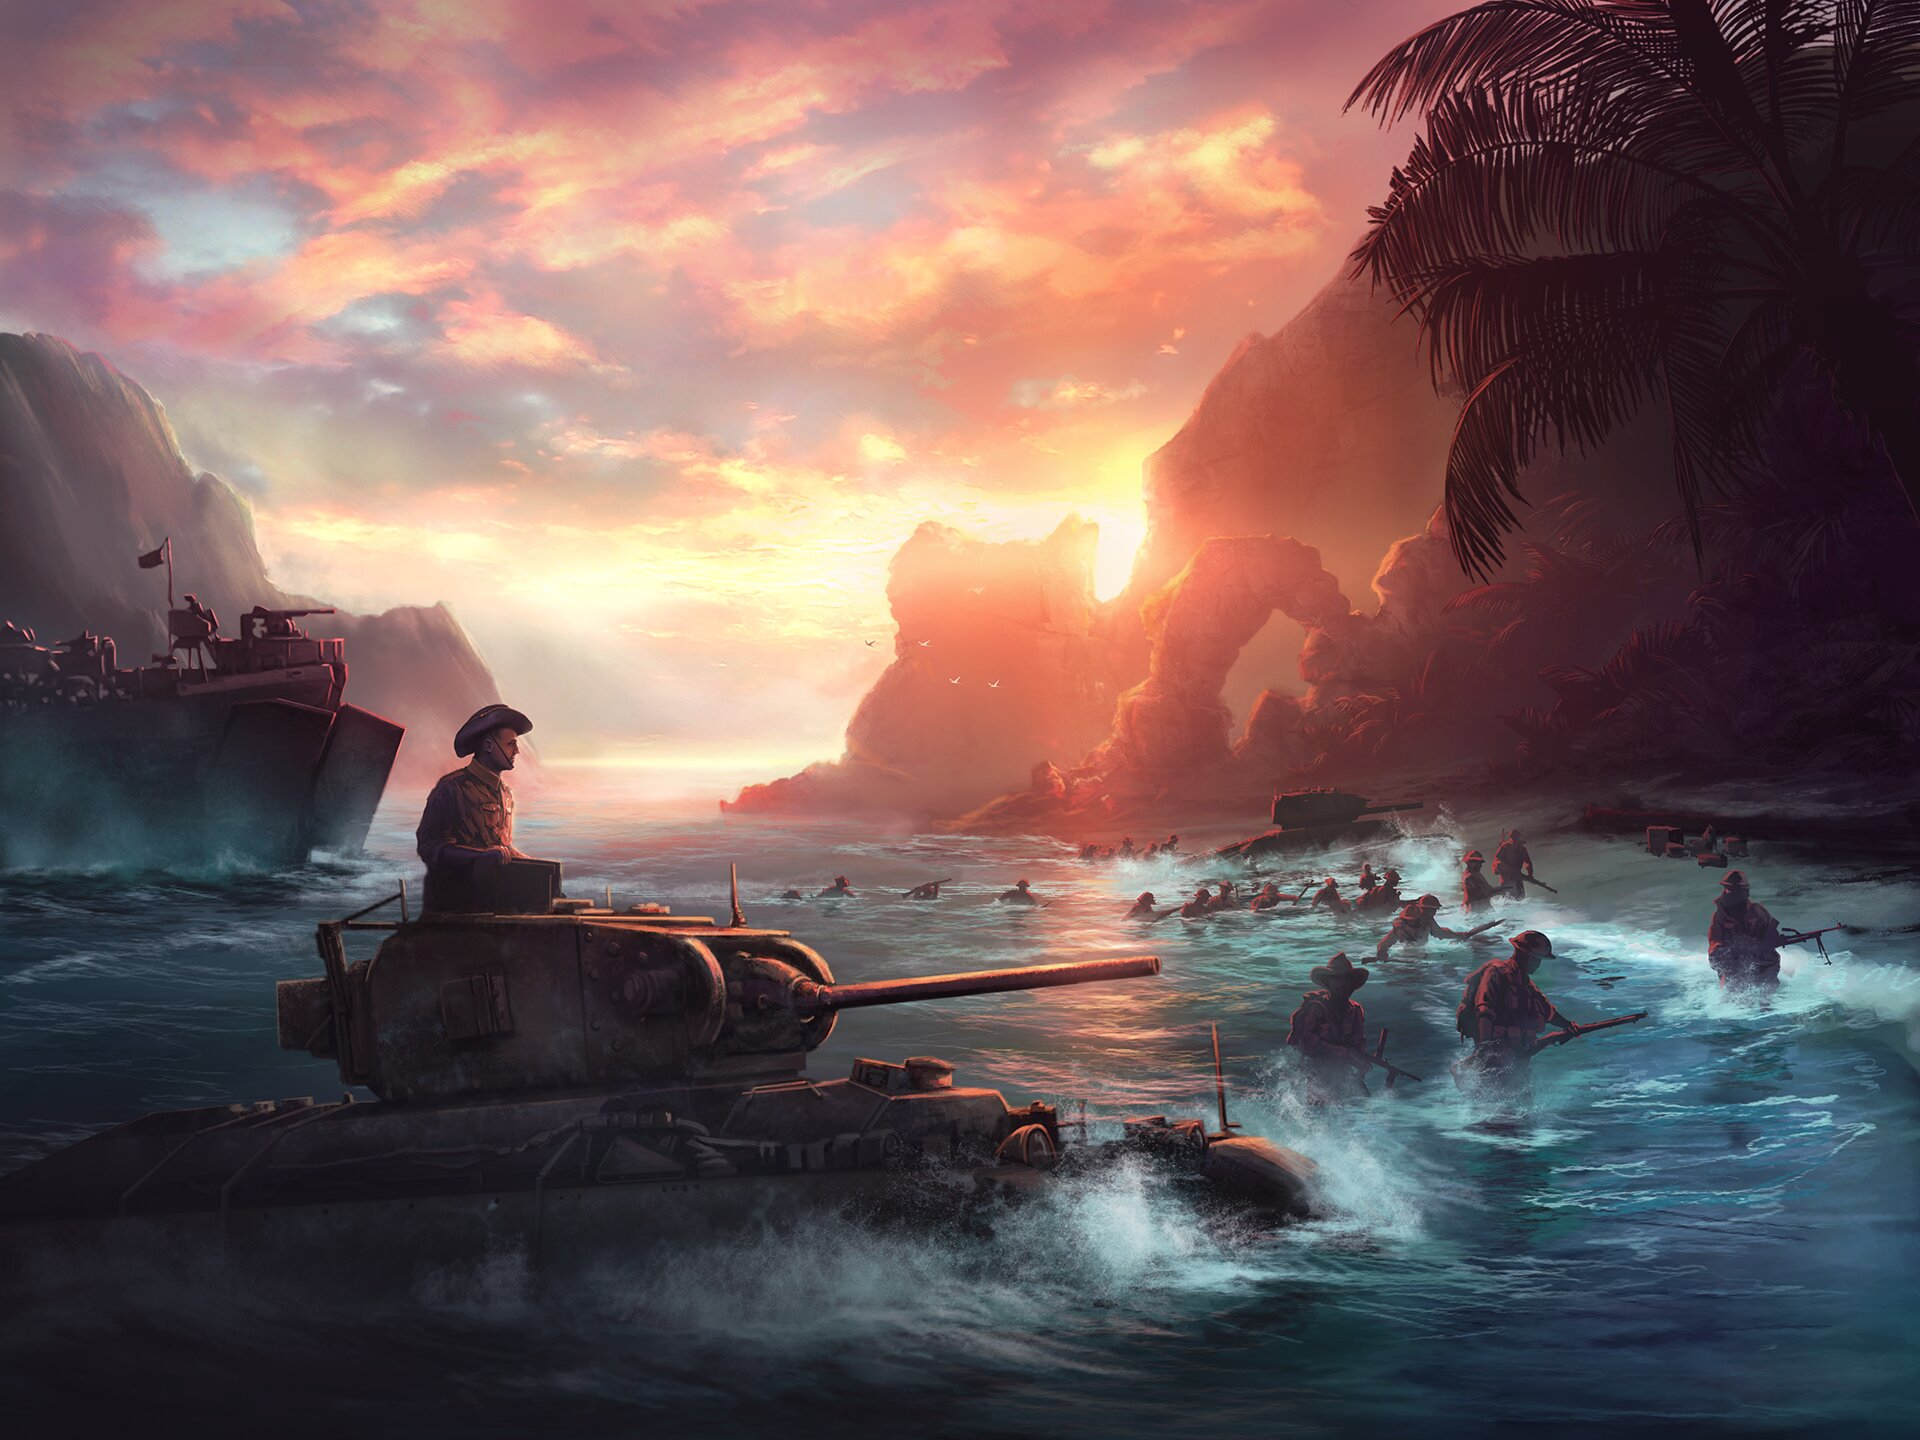
\includegraphics[width=\textwidth, frame]{cuerpo/cap-objetos/imagenes/hoi4-pacific-landing}
		\caption{Desembarco en el Pacífico.}
		\label{fig:hoi4-desembarco-pacifico}
	\end{subfigure}
	%
	\caption[Figura con 4 subfiguras.]{Figura con 4 subfiguras - ejemplo 1. Figuras alineadas inferiormente y en una matriz 2x2. Escenas de la Segunda Guerra Mundial. Fuente: \cite{hoi4}.}
	\label{fig:escenas-ww2}
\end{figure}
%
\newpage
\lstinputlisting[frame={single}, language={[AlLaTeX]TeX}, label={cod-fig:escenas-ww2}, caption=Código de la figura \ref{fig:escenas-ww2}.]{cuerpo/cap-objetos/codigos/subfigura3.txt}
%
\section{Figuras apaisadas}
\begin{figure}[H]
	\centering
	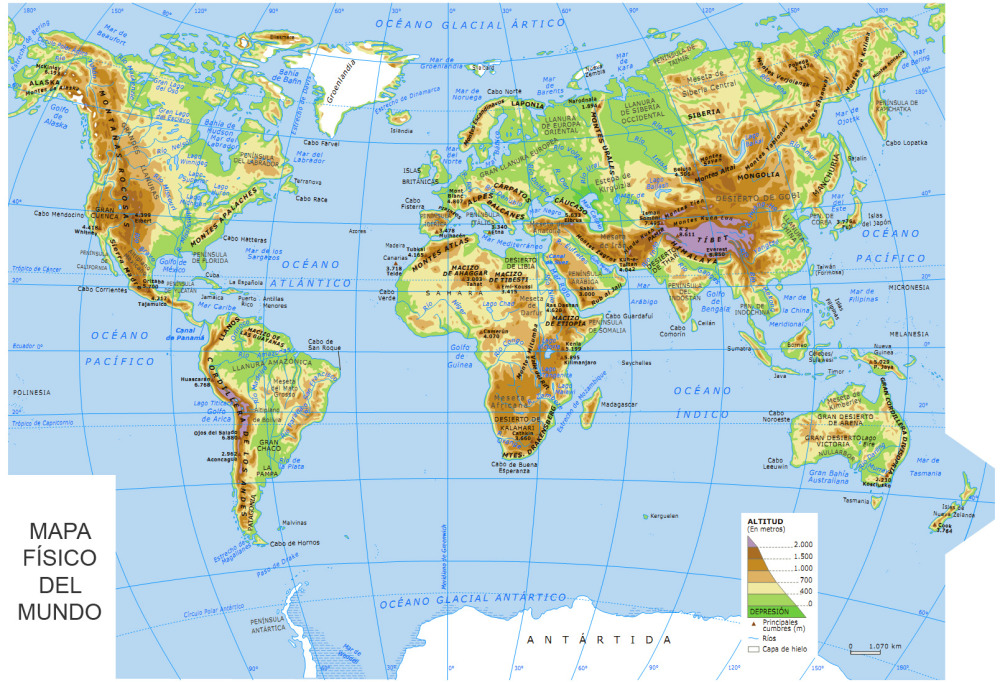
\includegraphics[width=\textwidth, frame]{cuerpo/cap-objetos/imagenes/mapa-fisico}
	\caption[Figura rotada 0.]{Figura rotada 0. Original: esta es la imagen en su posición original, con el tamaño ajustado al ancho de linea.}
	\label{fig:mapa-fisico-orig}
\end{figure}
\lstinputlisting[frame={single}, language={[AlLaTeX]TeX}, label={cod-fig:mapa-fisico-orig}, caption=Código de la figura \ref{fig:mapa-fisico-orig}.]{cuerpo/cap-objetos/codigos/apaisado0.txt}
%
\begin{figure}[H]
	\centering
	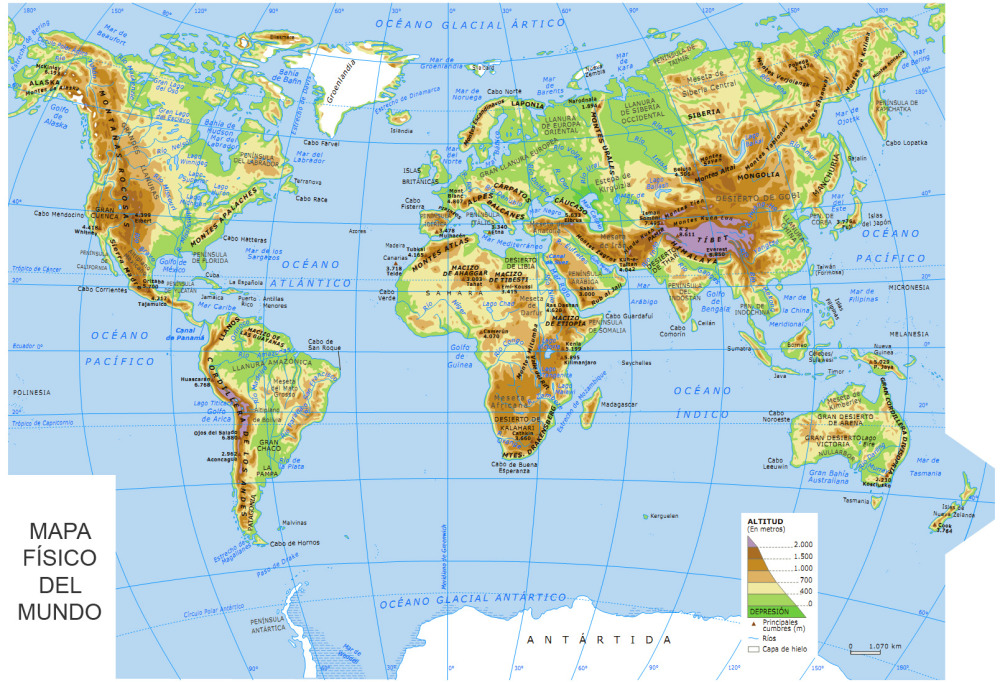
\includegraphics[width=\textwidth, frame, angle=90]{cuerpo/cap-objetos/imagenes/mapa-fisico}
	\caption[Figura rotada 1.]{Figura rotada 1. \textit{Método comando <<angle>>}: la imagen se rota 90\textdegree{} para aparecer apaisada, pero la página y el pie de página no. El tamaño se ha ajustado al ancho de linea.}
	\label{fig:mapa-fisico-a1}
\end{figure}
%\newpage
\lstinputlisting[frame={single}, language={[AlLaTeX]TeX}, label={cod-fig:mapa-fisico-a1}, caption=Código de la figura \ref{fig:mapa-fisico-a1}.]{cuerpo/cap-objetos/codigos/apaisado1.txt}
%
\begin{figure}[H]
	\centering
	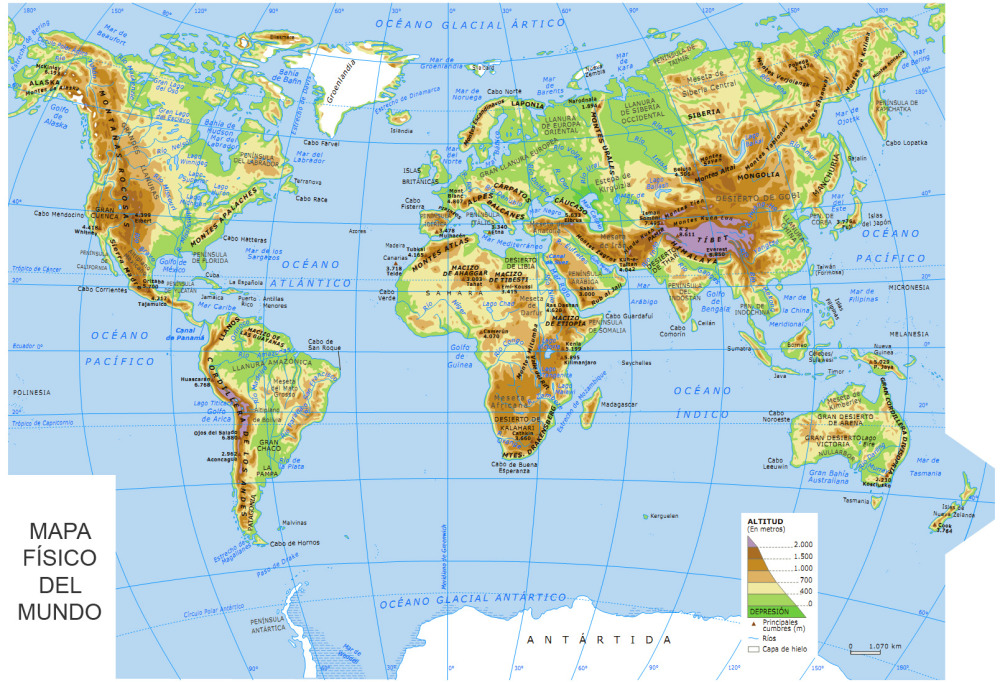
\includegraphics[scale=.65, frame, angle=90]{cuerpo/cap-objetos/imagenes/mapa-fisico}
	\caption[Figura rotada 2.]{Figura rotada 2.  \textit{Método comando <<angle>>}: la imagen se rota 90\textdegree{} para aparecer apaisada, pero la página y el pie de página no. El tamaño se ha ajustado a un 65\% del tamaño original.}
	\label{fig:mapa-fisico-a2}
\end{figure}
\newpage
\lstinputlisting[frame={single}, language={[AlLaTeX]TeX}, label={cod-fig:mapa-fisico-a2}, caption=Código de la figura \ref{fig:mapa-fisico-a2}.]{cuerpo/cap-objetos/codigos/apaisado2.txt}
%
\begin{sidewaysfigure}
	\centering
	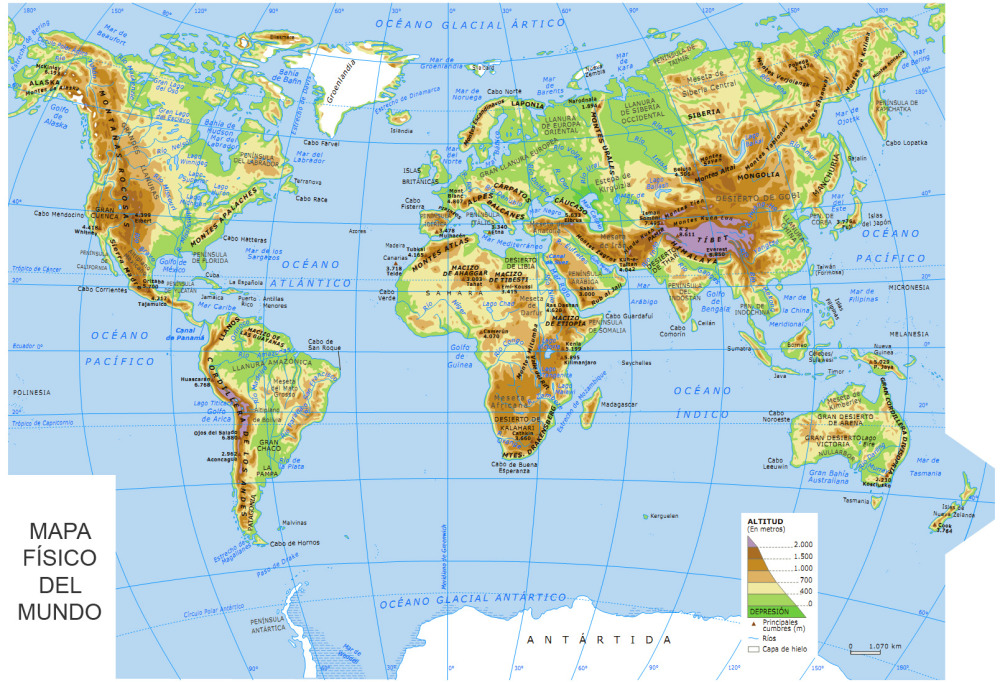
\includegraphics[width=\textwidth, frame]{cuerpo/cap-objetos/imagenes/mapa-fisico}
	\caption[Figura rotada 3.]{Figura rotada 3. \textit{Método entorno <<sidewaysfigure>>}: la imagen se rota automáticamente para aparecer apaisada, junto con el pie de página, pero la página en sí no. El tamaño se ha ajustado al ancho de linea.}
	\label{fig:mapa-fisico-a3}
\end{sidewaysfigure}
\lstinputlisting[frame={single}, language={[AlLaTeX]TeX}, label={cod-fig:mapa-fisico-a3}, caption=Código de la figura \ref{fig:mapa-fisico-a3}.]{cuerpo/cap-objetos/codigos/apaisado3.txt}
%
\begin{landscape}
	\begin{figure}[h]
		\centering
		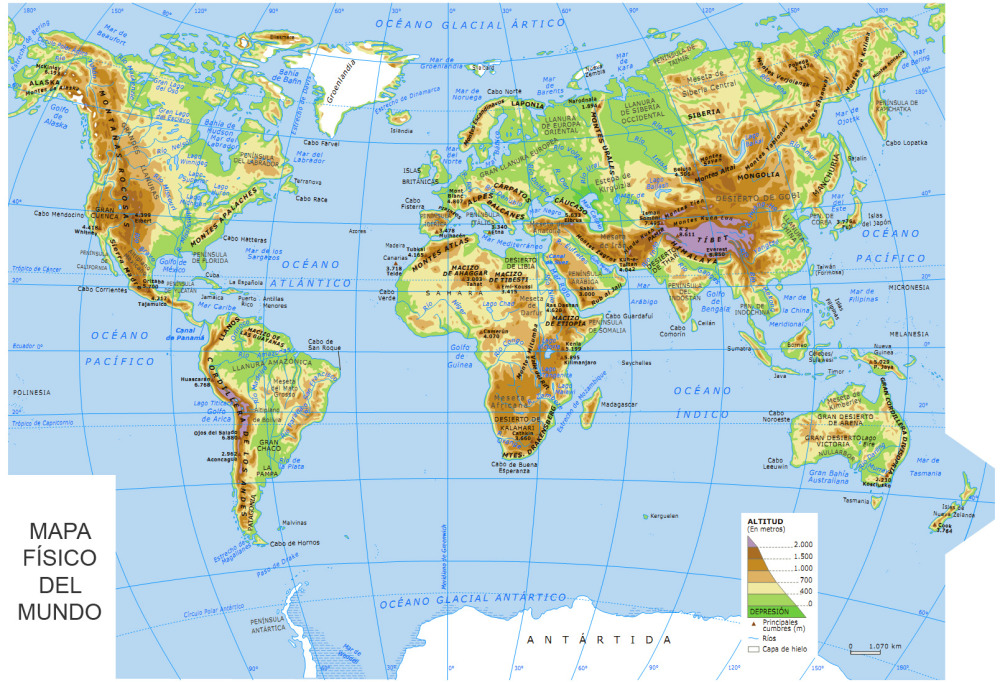
\includegraphics[scale=.65, frame, angle=0]{cuerpo/cap-objetos/imagenes/mapa-fisico}
		\caption[Figura rotada 4.]{Figura rotada 4. \textit{Método entorno <<landscape>>}: la página se rota automáticamente para aparecer apaisada incluido el pie de página, pero los encabezados no. El tamaño se ha ajustado a un 65\% del tamaño original. \hlc[green]{Método aconsejado}.}
		\label{fig:mapa-fisico-a4}
	\end{figure}
\end{landscape}
\lstinputlisting[language={[AlLaTeX]TeX}, label={cod-fig:mapa-fisico-a4}, caption=Código de la figura \ref{fig:mapa-fisico-a4}.]{cuerpo/cap-objetos/codigos/apaisado4.txt}
%
\begin{landscape}
	\begin{figure}
		\centering
		\begin{subfigure}[t]{.5\textwidth}
			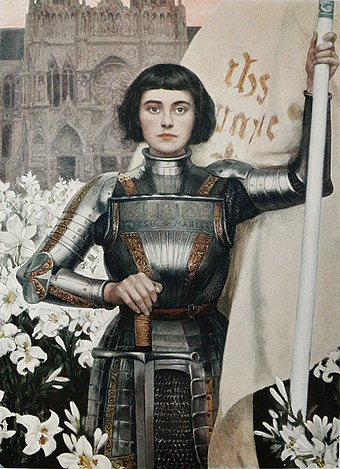
\includegraphics[width=\textwidth, frame]{cuerpo/cap-objetos/imagenes/juana-arco}
			\caption[Jean d´Arc]{Jean d´Arc. Grabado de Albert Lynch. Fuente: \cite{wikipedia-juana}.}
			\label{fig:juana-arco}
		\end{subfigure}
	%
		\begin{subfigure}[t]{0.5\textwidth}
			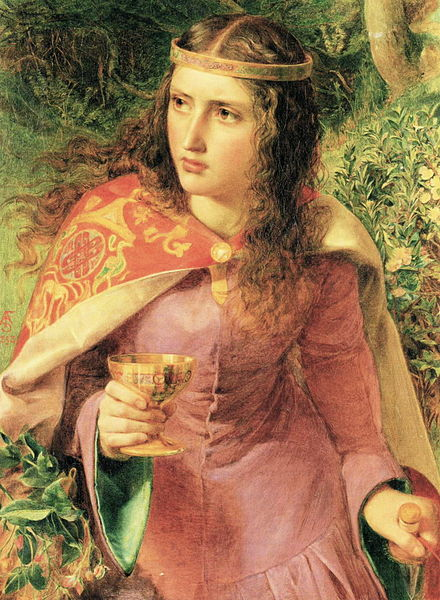
\includegraphics[width=\textwidth, frame]{cuerpo/cap-objetos/imagenes/eleanor-aquitania}
			\caption[Eleanor de Aquitania.]{Eleanor de Aquitania. Pintura de Frederick Sandys. Fuente: \cite{wikipedia-eleanor}.}
			\label{fig:eleanor-aquitania}
		\end{subfigure}
	\caption[Subfiguras en modo apaisado.]{Subfiguras en modo apaisado. Mujeres francesas del medievo.}
	\label{fig:subfiguras-apaisadas}
	\end{figure}
\end{landscape}
\lstinputlisting[frame={single}, language={[AlLaTeX]TeX}, label={cod-fig:subfiguras-apaisadas}, caption=Código de la figura \ref{fig:subfiguras-apaisadas}.]{cuerpo/cap-objetos/codigos/apaisado5.txt}
%
\chapter{Tablas}
3 opciones:
\begin{enumerate}
	\item Programar la tabla directamente; crear tablas en \LaTeX es complejo, no recomendado.
	\item Emplear una aplicación externa para crear la tabla en código \LaTeX e importarla al código; recomendaciones:
		\begin{itemize}
			\item  \href{https://www.tablesgenerator.com/}{https://www.tablesgenerator.com/}
			\item \href{https://www.latex-tables.com/}{https://www.latex-tables.com/}
		\end{itemize}
	\item Crear la imagen en un programa externo (hoja de cálculo, procesador de text, etc.) e incluirla como una imagen dentro de un entorno de tabla.
\end{enumerate}
%
\begin{table}[H]
	\centering
	\begin{tabular}{@{}lll@{}}
		\toprule
		Variable & Valor & Unidad \\ \midrule
		X        & 20    & N      \\
		Y        & 100   & kg     \\
		Z        & 0     & cm     \\ \bottomrule
	\end{tabular}
	\caption[Tabla creada con \url{https://www.tablesgenerator.com/}.]{Tabla creada con \url{https://www.tablesgenerator.com/}. Copiada directamente al \LaTeX.}
	\label{tab:tabla-1}
\end{table}
%
%tab:tabla-2
\begin{table}[H]
	\centering
	\begin{tabular}{@{}lll@{}}
		\toprule
		Variable & Valor & Unidad \\ \midrule
		A        & 0    & N      \\
		B        & 100   & kg     \\
		C        & 20     & cm     \\ \bottomrule
	\end{tabular}
	\caption[Tabla creada con \url{https://www.tablesgenerator.com/} bis]{Tabla creada con \url{https://www.tablesgenerator.com/} bis. El código se pega en un .tex específico y se importa al \LaTeX.}
	\label{tab:tabla-2}
\end{table}
%
\begin{table}[H]
	\centering
	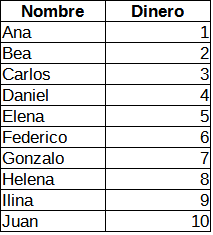
\includegraphics[scale=1]{cuerpo/cap-objetos/tablas/tabla-imagen-calc}
	\caption{Tabla desde una imagen.}
	\label{tab:tabla-3}
\end{table}

\begin{table}[H]
	\centering
	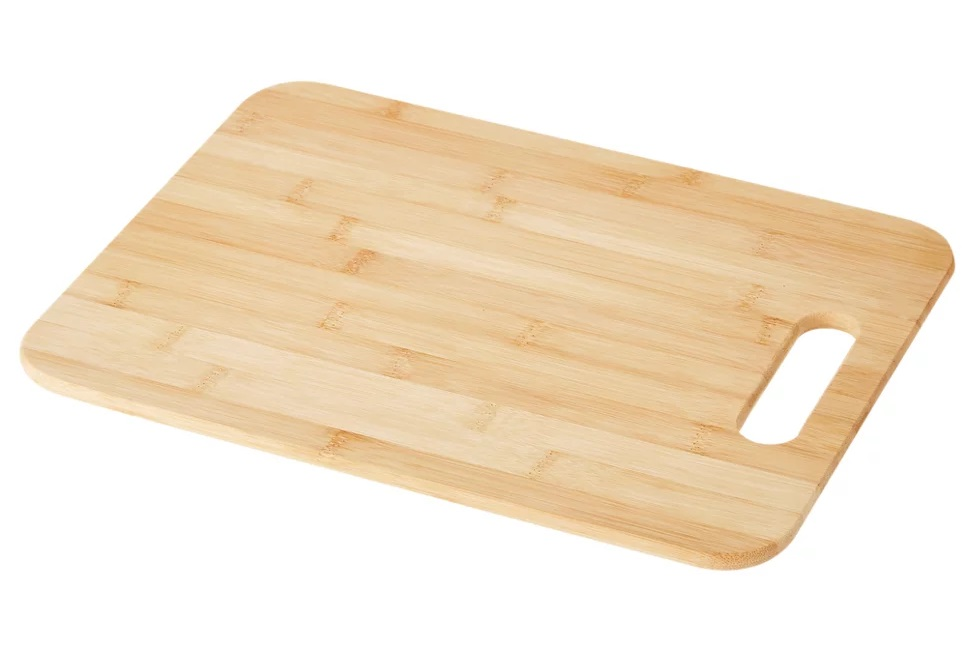
\includegraphics[width=1\textwidth, frame]{cuerpo/cap-objetos/tablas/tablas}
	\caption[Tabla desde una imagen bis.]{Tabla desde una imagen bis. Esta imagen es tratada como una tabla, apareciendo en el índice de tablas, y contando como tal par las referencias. La diferencia entre los entornos 'table' y 'figure' es puramente de distinción de items.}
	\label{tab:tabla-4}
\end{table}
\newpage
El código empleado es el mostrado en el fragmento \ref{cod-tablas}.
\lstinputlisting[frame={single}, language={[AlLaTeX]TeX}, label={cod-tablas}, caption=Código empleado para las tablas \ref{tab:tabla-1} a \ref{tab:tabla-2}.]{cuerpo/cap-objetos/codigos/tablas.txt}
%
\chapter{Documentos .pdf}
Los pdf se incluyen con el paquete \textit{pdfpages}, y su comando:
\lstinputlisting[language ={[AlLaTeX]TeX} , label ={cod-pdf} , caption ={
	Comando para incluir un documento .pdf. } , frame ={ single } , float ]{cuerpo/cap-objetos/codigos/include-pdf.txt}

\chapter{Planos}
%El sistema implementado en la plantilla está diseñado bajo 2 premisas:
\begin{enumerate}
	\item Los planos origen serán archivos .pdf.
	\item Los planos se agrupan por conjuntos, siendo estos los que aparecen en el índice de contenidos; y se crea índice de planos específico.
\end{enumerate}

Comandos y sintaxis:
\begin{enumerate}
	\item Crear e imprimir el índice de planos; estos comandos se deben insertar donde se quiera que aparezca el índice de planos.
	\lstinputlisting[frame={single}, language={[AlLaTeX]TeX}, label={cod-planos1}, caption=Comandos para el índice de planos]{cuerpo/cap-objetos/codigos/planos1.txt}
	%
	\item Invocar una nueva entrada en el índice de planos para separar conjuntos de planos.
	\lstinputlisting[frame={single}, language={[AlLaTeX]TeX}, label={cod-planos2}, caption=Comandos para crear un conjunto de planos que quedarán agrupados bajo una misma sección. Es esta etiqueta la que aparecerá en el índice de planos.]{cuerpo/cap-objetos/codigos/planos2.txt}
	\item Invocar una nueva entrada de plano.
	\lstinputlisting[frame={single}, language={[AlLaTeX]TeX}, label={cod-planos3}, caption=Comandos para invocar e incluir un nuevo plano.]{cuerpo/cap-objetos/codigos/planos1.txt}
\end{enumerate}
Se ha creado una macro para generar los pasos 2 y 3, disponible en el menú <<Macros>> del perfil, de nombre <<Add blueprint>>.
%
\chapter{Código}
Se puede incluir código de forma que sea tratado como un objeto, para crear un índice y usar referencias, e incluso resaltar palabras clave del lenguaje.

El método recomendado es mediante el paquete \href{https://www.ctan.org/pkg/listings}{\textit{listings}}. Se ha creado la macro <<Include code>> (y su botón correspondiente) en el perfil de TeXstudio para importar código desde archivos externos, que inserta el comando del fragmento \ref{cod-codigo-comando}:
\lstinputlisting[frame={single}, language={[AlLaTeX]TeX}, label={cod-codigo-comando}, caption=Linea insertada por la macro <<Include code>>.]{cuerpo/cap-objetos/codigos/codigo-comando.txt}

Se puede personalizar al cargar el paquete, en el archivo \textit{.../02-paquetes.tex} (colores, fuente, etc.).
%
\chapter{Expresiones matemáticas}
Las expresiones matemáticas son parte del código \LaTeX{} del documento, que se teclean directamente en el .tex, y dentro del modo matemático o en el entorno \textit{equation}. Cambian la tipografía a la matemática y activan comandos específicos para símbolos demás.
%
\section{Entorno matemático}\label{sec:entorno-matematico}
O \textit{math environment} o \textit{math mode}; su comportamiento por defecto es <<en linea>>, lo que permite alternarlo con modo texto; se activa encerrando la expresión deseada entre los símbolos \$\$.

Por ejemplo, si esto es un párrafo en el cual queremos integrar una expresión matemática como $ y = mb + c$, de forma que quede en linea con el resto del texto.
\lstinputlisting[frame={single}, language={[AlLaTeX]TeX}, label={cod-entorno-mat}, caption=Código del párrafo \ref{sec:entorno-matematico}.]{cuerpo/cap-objetos/codigos/mates-entorno-mat.txt}
%
\section{Entorno ecuación}
\textit{equation environment}, es un entorno de \LaTeX{} que imprime expresiones, por defecto, en una línea aparte, centrada, y opcionalmente con etiqueta para numerar. Se puede acceder mediante los botones mostrados en la figura \ref{fig:toolbar-lat}.

En este párrafo ponemos unos ejemplos; lorem ipsum lorem ipsum lorem ipsum; y aquí queremos una expresión matemática numerada:
\begin{equation}\label{ec-2-ley-newton}
	\sum \vec{F} = m \cdot \vec{a}
\end{equation}
Otro ejemplo más:
\begin{equation}\label{ec-einstein}
	e = mc^{2}
\end{equation}

Y para que no lleven etiqueta de numeración:
\begin{equation*}\label{ec-ley-ohm}
	V = I \cdot R
\end{equation*}
\lstinputlisting[frame={single}, language={[LaTeX]TeX}, label={cod-ecs}, caption=Código para expresiones matemáticas]{cuerpo/cap-objetos/codigos/mates-entorno-ecs.txt}
%
\chapter{Enumeraciones}
%
\begin{figure}[H]
	\centering
	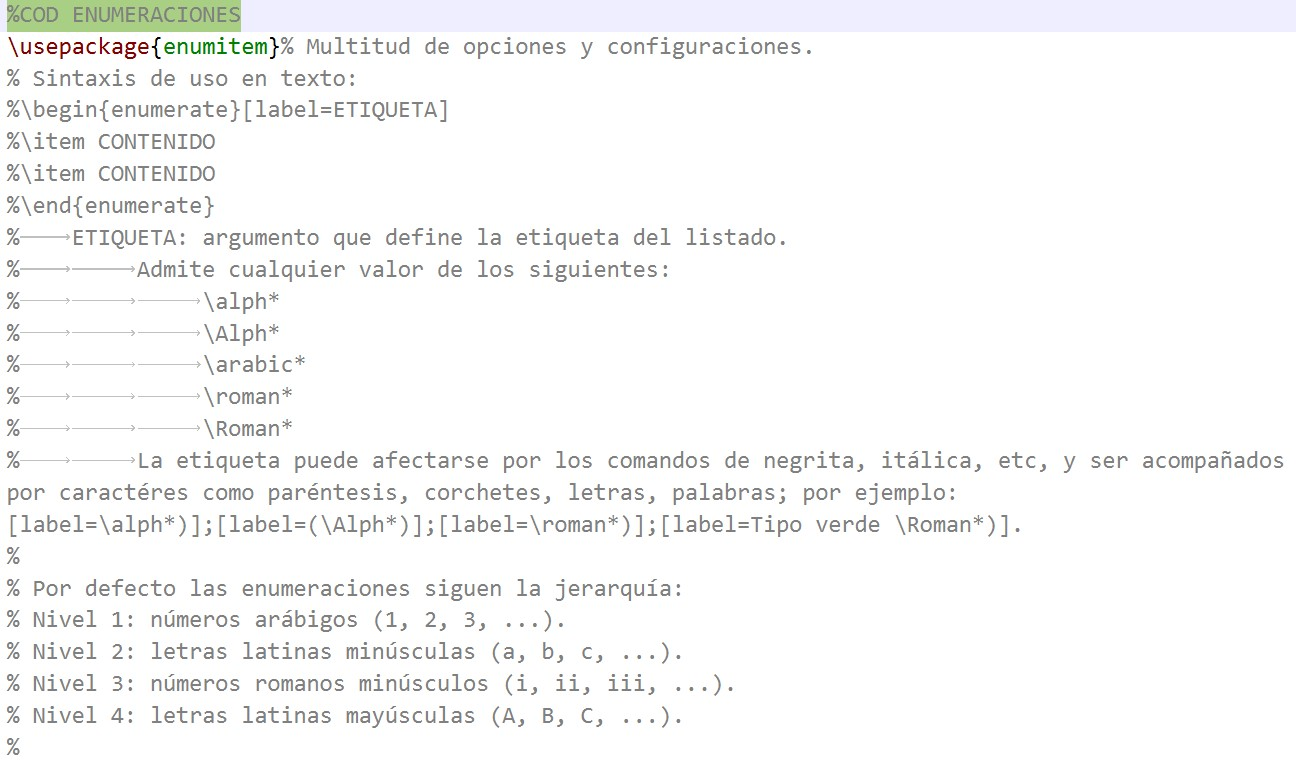
\includegraphics[width=1\linewidth, frame]{cuerpo/cap-objetos/imagenes/enumeraciones}
	\caption[Configuración de las enumeraciones.]{Configuración de las enumeraciones. Sintaxis para personalizar las enumeracions. Archivo: .../02-paquetes.tex.}
	\label{fig:enumeraciones}
\end{figure}
%
%
\begin{itemize}
\item\textbf{Enumeración por defecto:}
	\begin{enumerate}
		\item Elemento.
		\item Elemento.
		\item Elemento.
		\item Elemento.
		\item Elemento.
		\item Elemento.
		\item Elemento.
		\item Elemento.
	\end{enumerate}
%
\item\textbf{Enumeración por defecto en varias columnas:}
	\begin{multicols}{3}
		\begin{enumerate}
		\item Elemento.
		\item Elemento.
		\item Elemento.
		\item Elemento.
		\item Elemento.
		\item Elemento.
		\item Elemento.
		\item Elemento.
	\end{enumerate}
\end{multicols}
%
\item\textbf{Enumeración personalizada para usar letras minúsculas con paréntesis de cierre:}
	\begin{enumerate}[label=\alph*)]
		\item Elemento.
		\item Elemento.
		\item Elemento.
		\item Elemento.
	\end{enumerate}
%
\item\textbf{Enumeración personalizada para usar numeral romano precedido de la palabra <<caca>>:}
	\begin{enumerate}[label=caca \Roman*]
		\item Elemento.
		\item Elemento.
		\item Elemento.
		\item Elemento.
	\end{enumerate}
\end{itemize}
%
\chapter{Hiperenlaces}
Los hiperenlaces se incluyen mediante el paquete \textit{hyperref}; mediante el comando:
\begin{center}
	\textbackslash href \{URL\}\{TEXTO\}
\end{center}

Por ejemplo \href{https://en.wikipedia.org}{este enlace lleva a Wikipedia.}
%
\part{Uso y gestión de referencias}
\chapter{Gestión de la bibliografía}
La bibliografía se configura en 3 archivos:
\begin{enumerate}
	\item \textit{.../configuracion/05-gestion-bibliografia.tex}: configura la bibliografía y carga las referencias a través de los archivos .BIB.
	\item \textit{.../bibliografia/bibliografia.tex}: carga los comandos de impresión de la bibliografía.
	\item \textit{Archivos .BIB}: son archivos de texto en los que se almacenan las referencias bibliográficas; para la plantilla se guardan en \textit{.../bibliografia/}.
\end{enumerate}
%

La plantilla separa la bibliografía finalmente impresa en 3 partes:
\begin{enumerate}
	\item \textbf{Referencias}: para las obras citadas en el \LaTeX; automatizado.
	\item \textbf{Bibliografía}: para las obras no citadas en el \LaTeX; automatizado.
	\item \textbf{Normativa}: requiere incluir la \textit{keyword} <<nor>> en cada elemento del .BIB que se quiera incluir en esta categoría.
\end{enumerate}
%
\begin{figure}[h]
	\centering
	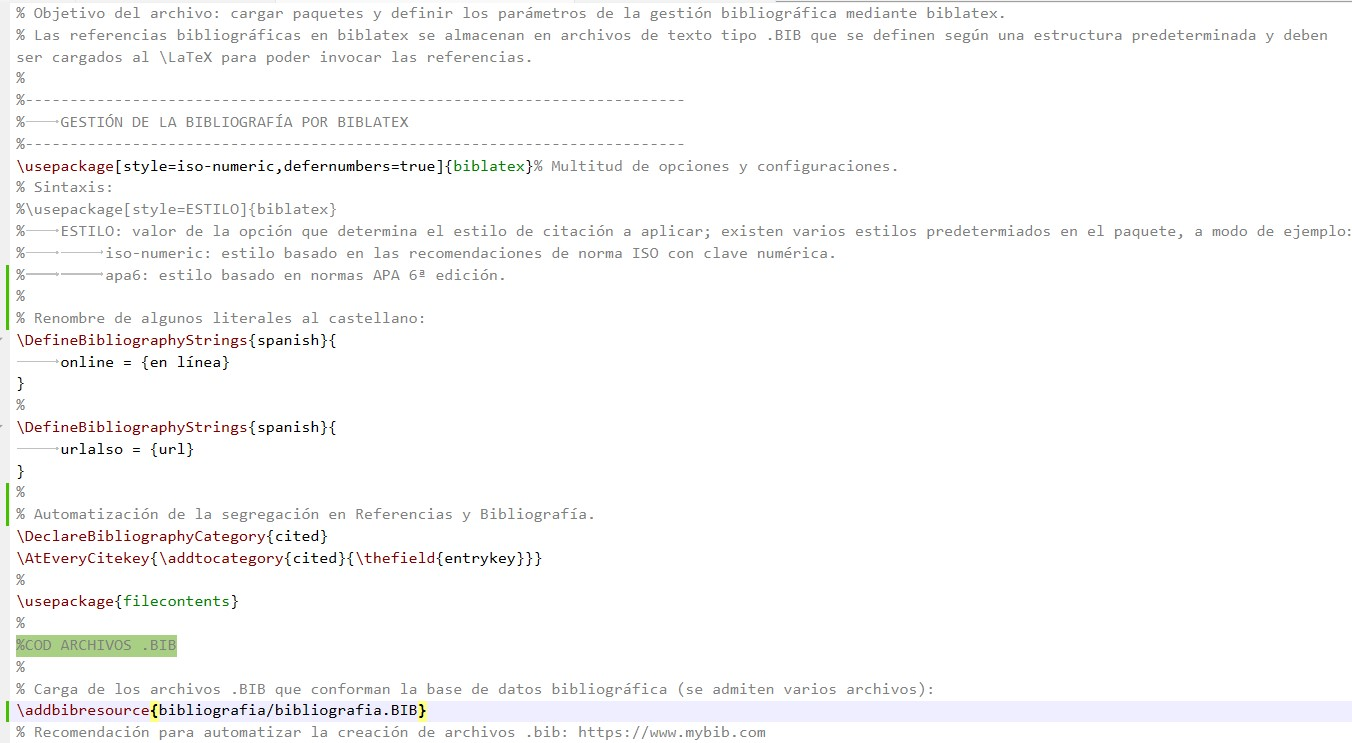
\includegraphics[width=1\linewidth, frame]{cuerpo/cap-referencias/imagenes/05-gestion}
	\caption[Configuración de la gestión bibliográfica.]{Configuración de la gestión bibliográfica. Aquí se carga el paquete y las opciones fundamentales para gestionar la bibliografía, y también los archivos .BIB. Archivo: \textit{.../configuracion/05-gestion-bibliografica.tex}.}
	\label{fig:05-gestion}
\end{figure}
%
\begin{figure}[h]
	\centering
	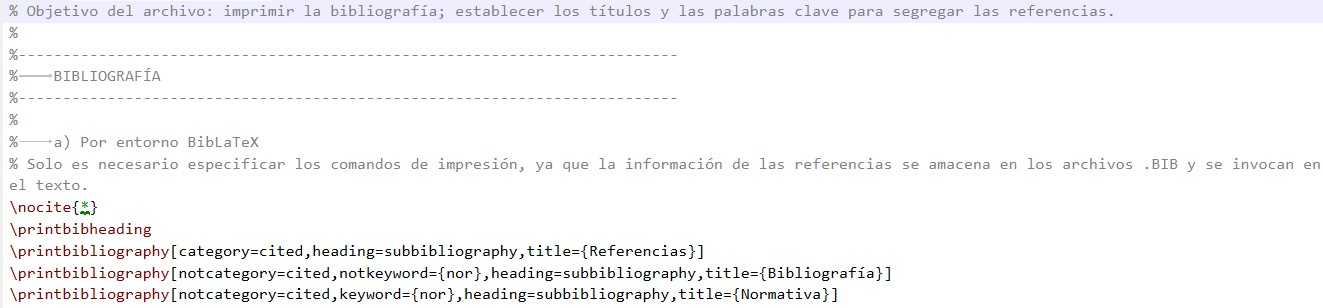
\includegraphics[width=1\linewidth, frame]{cuerpo/cap-referencias/imagenes/biblatex}
	\caption[Configuración de la impresión bibliográfica.]{Configuración de la impresión bibliográfica. Aquí se implementan los comandos de impresión. Archivo: \textit{.../bibliografia/bibliografia.tex}.}
	\label{fig:biblatex}
\end{figure}
%
\begin{figure}[h]
	\centering
	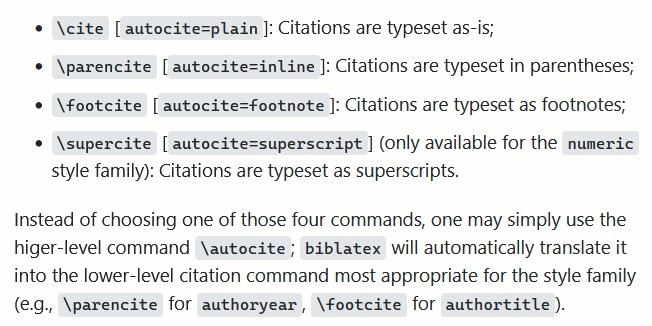
\includegraphics[width=1\linewidth, frame]{cuerpo/cap-referencias/imagenes/modos-cita}
	\caption[Comandos para citar obras.]{Comandos para citar obras.}
	\label{fig:modos-cita}
\end{figure}
%
\chapter{Referencias internas}
Las referencias internas se basan en las etiquetas (\textit{label}). A cada elemento latex (imagen, tabla, sección, párrafo, etc.) se le puede asignar una etiqueta simplemente escribiendo el comando \textit{\textbackslash label\{\}} a su comienzo, o dentro de su entorno. Después, se puede hacer una referencia haciendo una llamada a la etiqueta con el comando \textit{\textbackslash ref\{\}}.

\chapter{Ejemplos de referencias y citas}\label{cap:ejemplos de referencias y citas}
Este es un párrafo sobre Julio César, y en este punto citamos un dato sobre la guerra de las Galias que hemos sacado de una edición de \textit{De bello Gallico}, el dato es X \cite{juliocesar}. Esta guerra acabó tras el asedio de Alesia, con la rendición de los galos liderados por Vercingetorix, escena recreada en el cuadro \ref{fig:rendicion-alesia}. El código empleado se muestra en el fragmento \ref{cod-cesar}.

\begin{figure}[h]
	\centering
	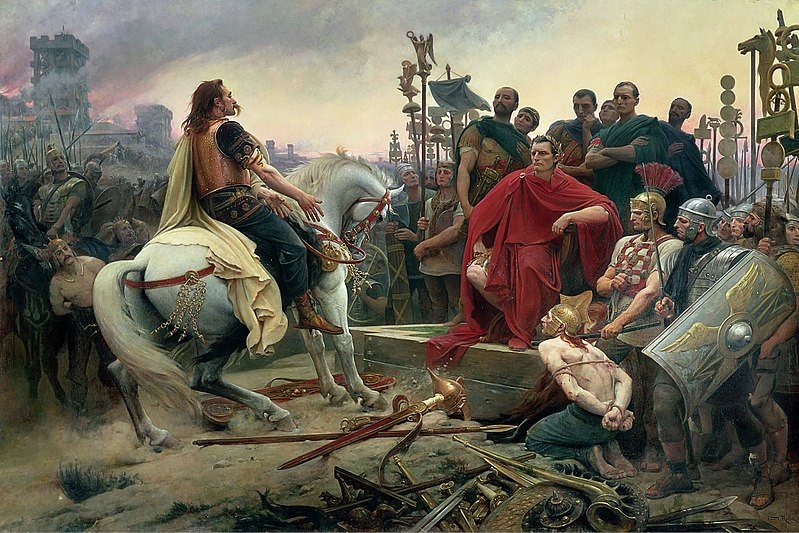
\includegraphics[width=1\linewidth, frame]{cuerpo/cap-referencias/imagenes/rendicion-alesia}
	\caption[Vercingetorix rinde sus armas a los pies de Julio César.]{Vercingetorix rinde sus armas a los pies de Julio César. Cuadro de Lionel Royer. Fuente: \cite{cuadro-rendicion-alesia}.}
	\label{fig:rendicion-alesia}
\end{figure}
%
\newpage
\lstinputlisting[frame={single}, language={[AlLaTeX]TeX},, label={cod-cesar}, caption=Código empleado en el capítulo \ref{cap:ejemplos de referencias y citas}.]{cuerpo/cap-referencias/codigos/cesar.txt}
%
\part{Fuentes de información}
\chapter{Fuentes de información}
\begin{enumerate}
	\item \href{https://es.overleaf.com/learn}{Overleaf}: editor en-linea y en la nube, cuya web ofrece guías, tutoriales y plantillas.
	%
	\item \href{https://www.ctan.org/}{CTAN}: web donde la comunidad sube paquetes.
	%
	\item \href{https://tex.stackexchange.com}{Latex Stack Exchange}: web de preguntas y respuestas.
	%
	\item \url{https://www.latextemplates.com/}: web con plantillas varias.
\end{enumerate}

%
%--------------------------------------------------------------------------
%COD	PLANOS
%--------------------------------------------------------------------------
\addtocontents{toc}{\protect\setcounter{tocdepth}{0}}% Modificar la profundidad del Índice de Contenidos, desde este línea en adelante incluir solo hasta \chapter; así no salen los planos individuales en el ToC general, si no por Conjunto de planos (Capítulos).
%
% Objetivo del archivo: imprimir los planos que se quieran inlcuir como un conjunto.
%
% Sintaxis:
% Incluir un título de conjunto para el índice de planos:
%\conjuntoplanos{Texto del título del conjunto}
%
% Incluir un título de plano:
%\plano{Texto del título del plano}
% Inlcuir un plano como .pdf:
%\begin{figure}
%	\includepdf[scale=X, landscape, pagecommand={}]{RUTA}
%\end{figure}
%
\part{Planos}
%
\conjuntoplanos{Colegio de prácticas del Máster de Incendios}
%
\plano{Planta Baja}
\begin{figure}
	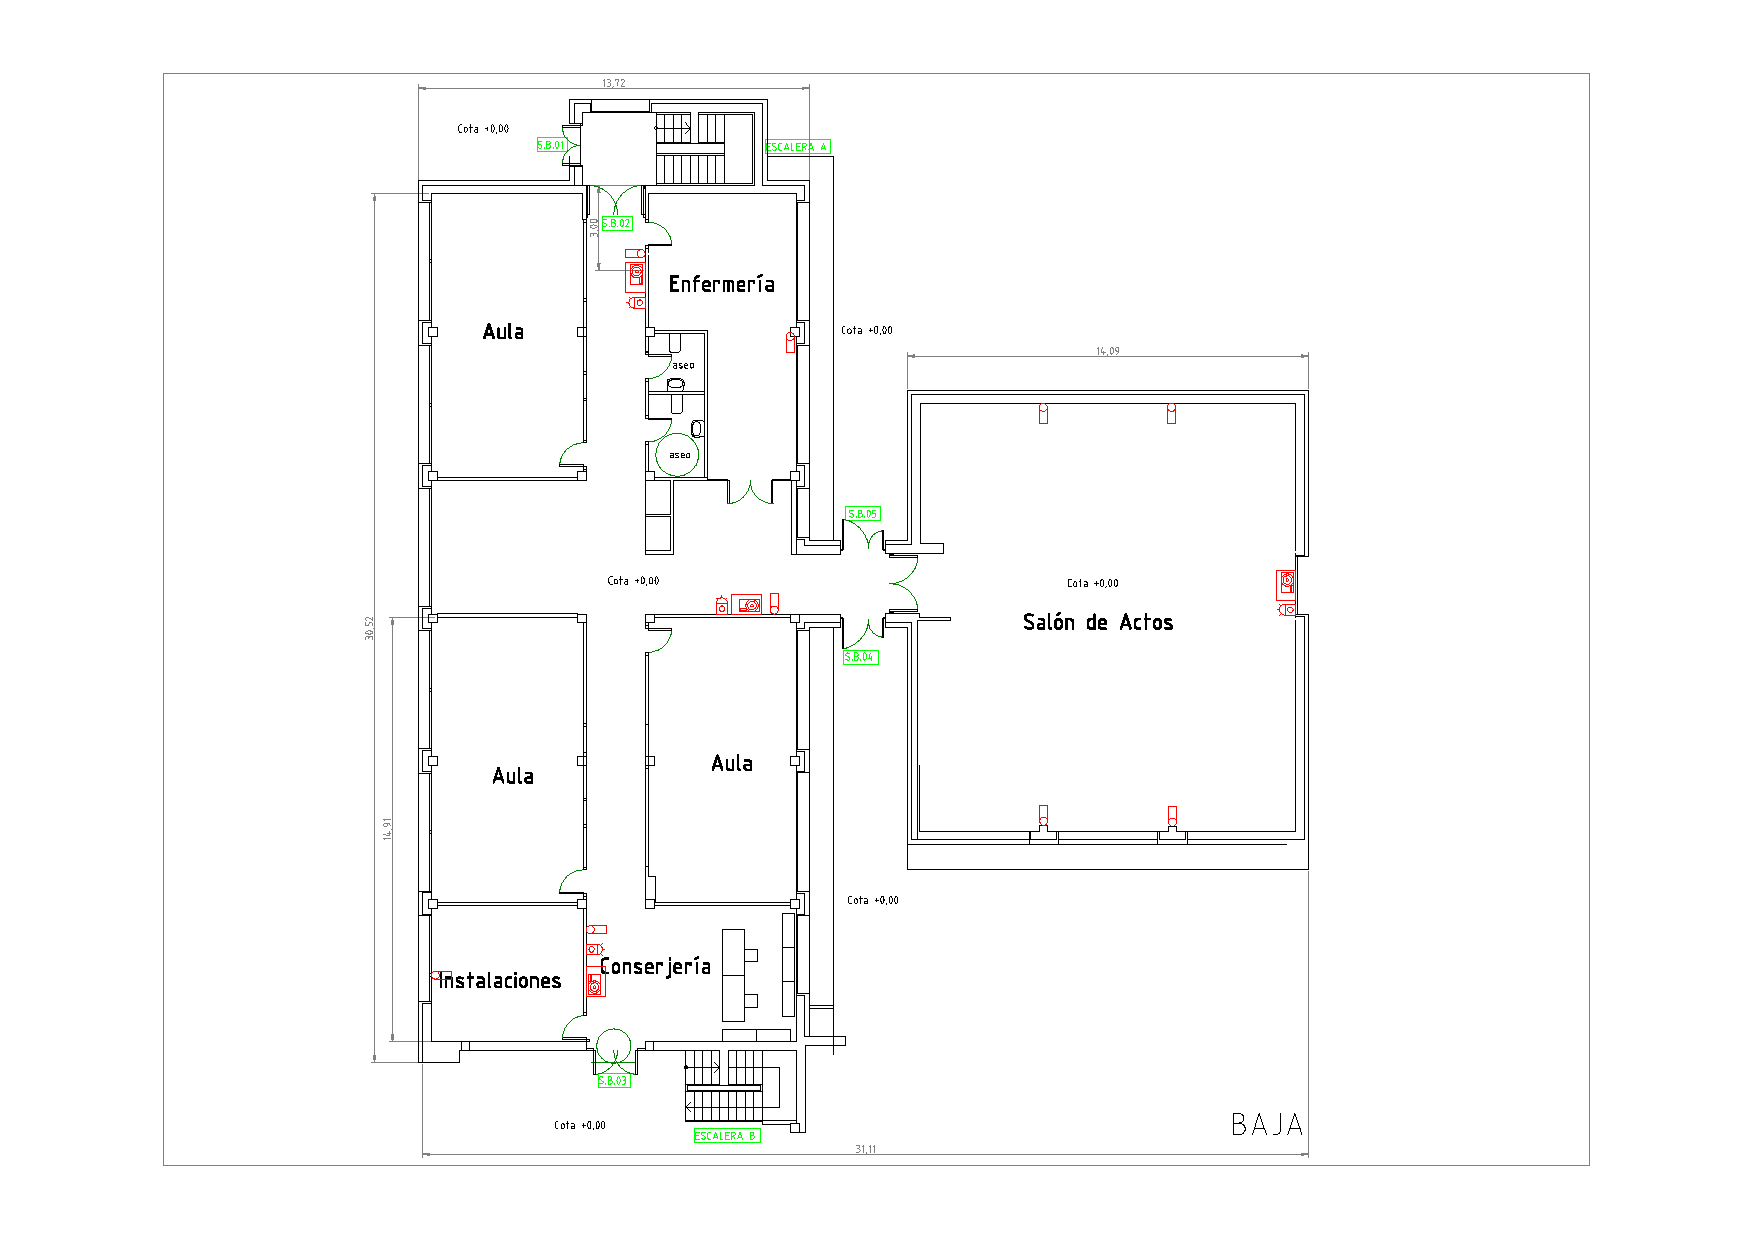
\includepdf[scale=0.95, landscape, pagecommand={}]{planos/plano-planta0.pdf}
\end{figure}
%%
\plano{Planta Primera}
\begin{figure}
	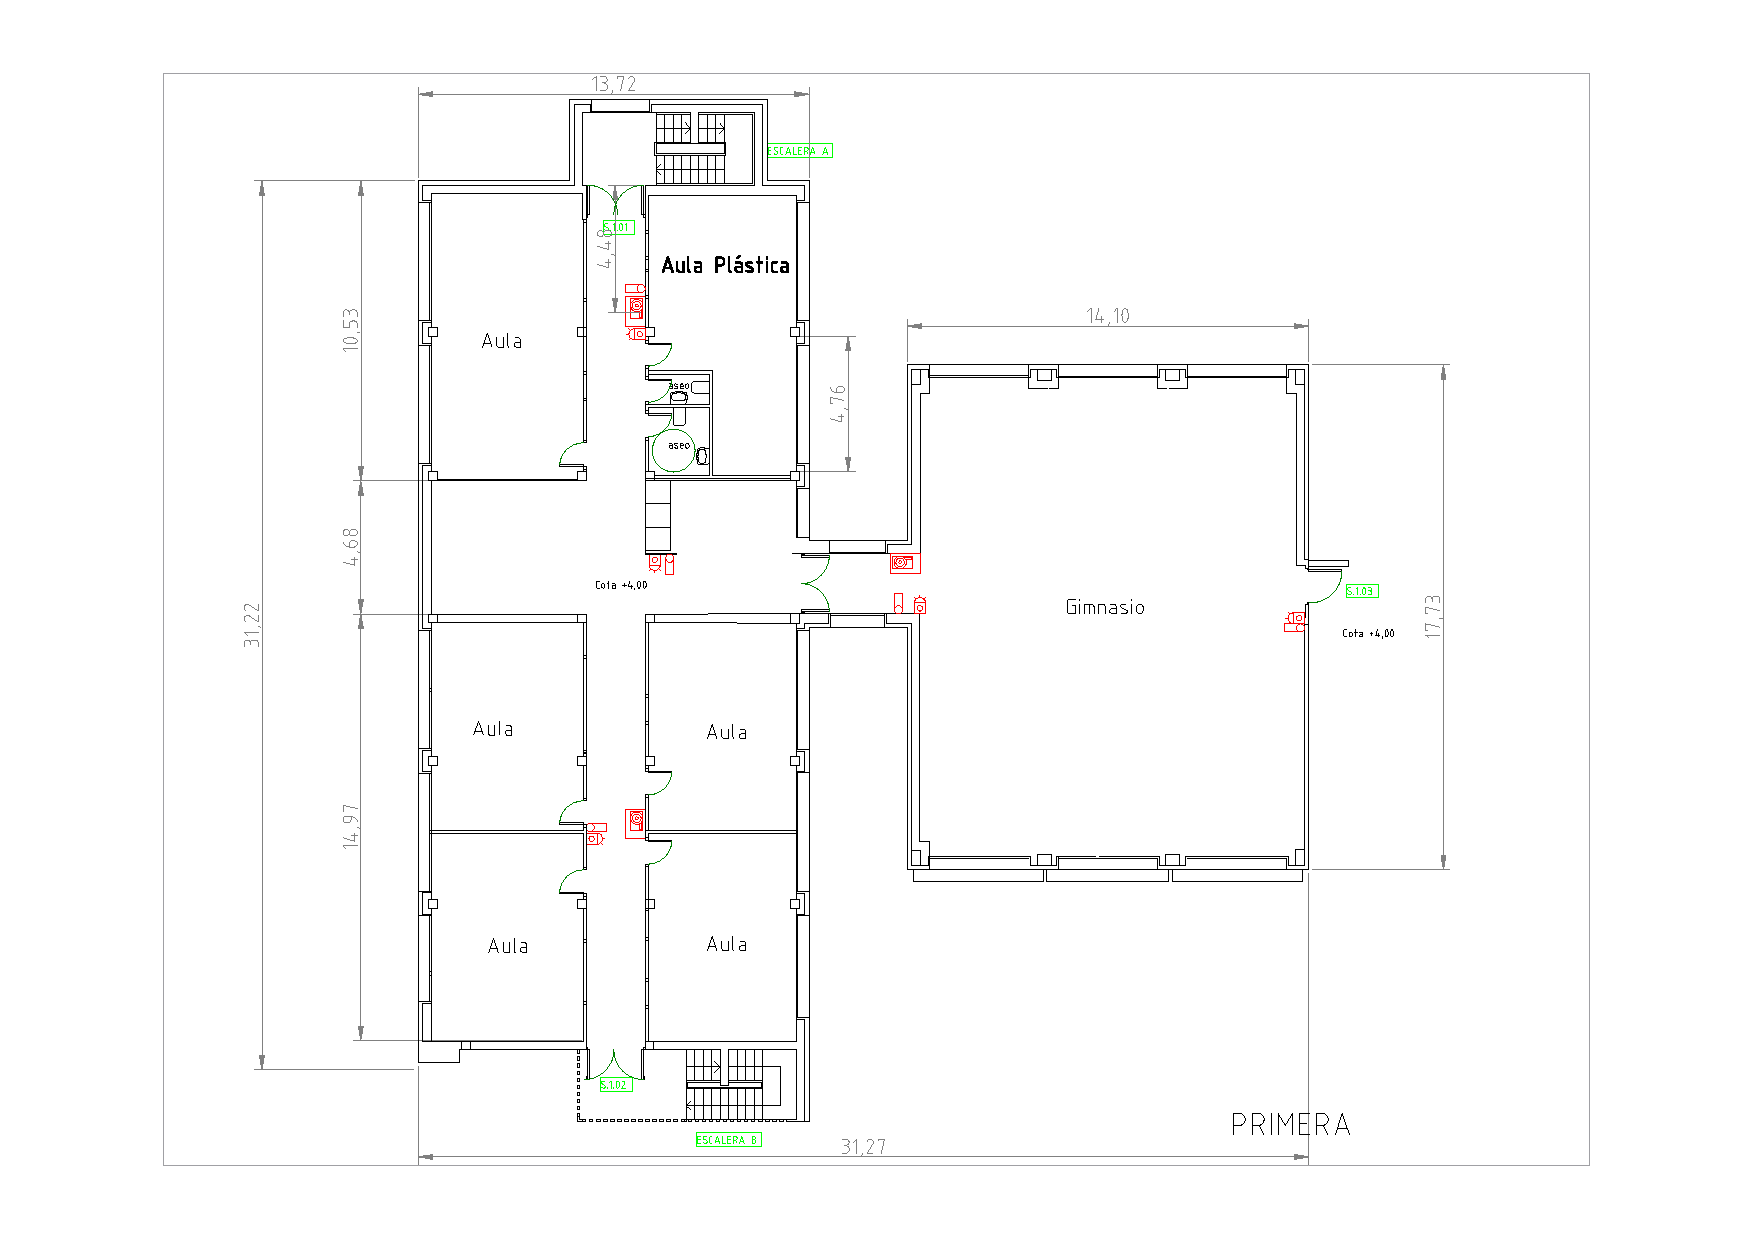
\includepdf[scale=0.95, landscape, pagecommand={}]{planos/plano-planta1.pdf}
\end{figure}
%
\plano{Planta Segunda}
\begin{figure}
	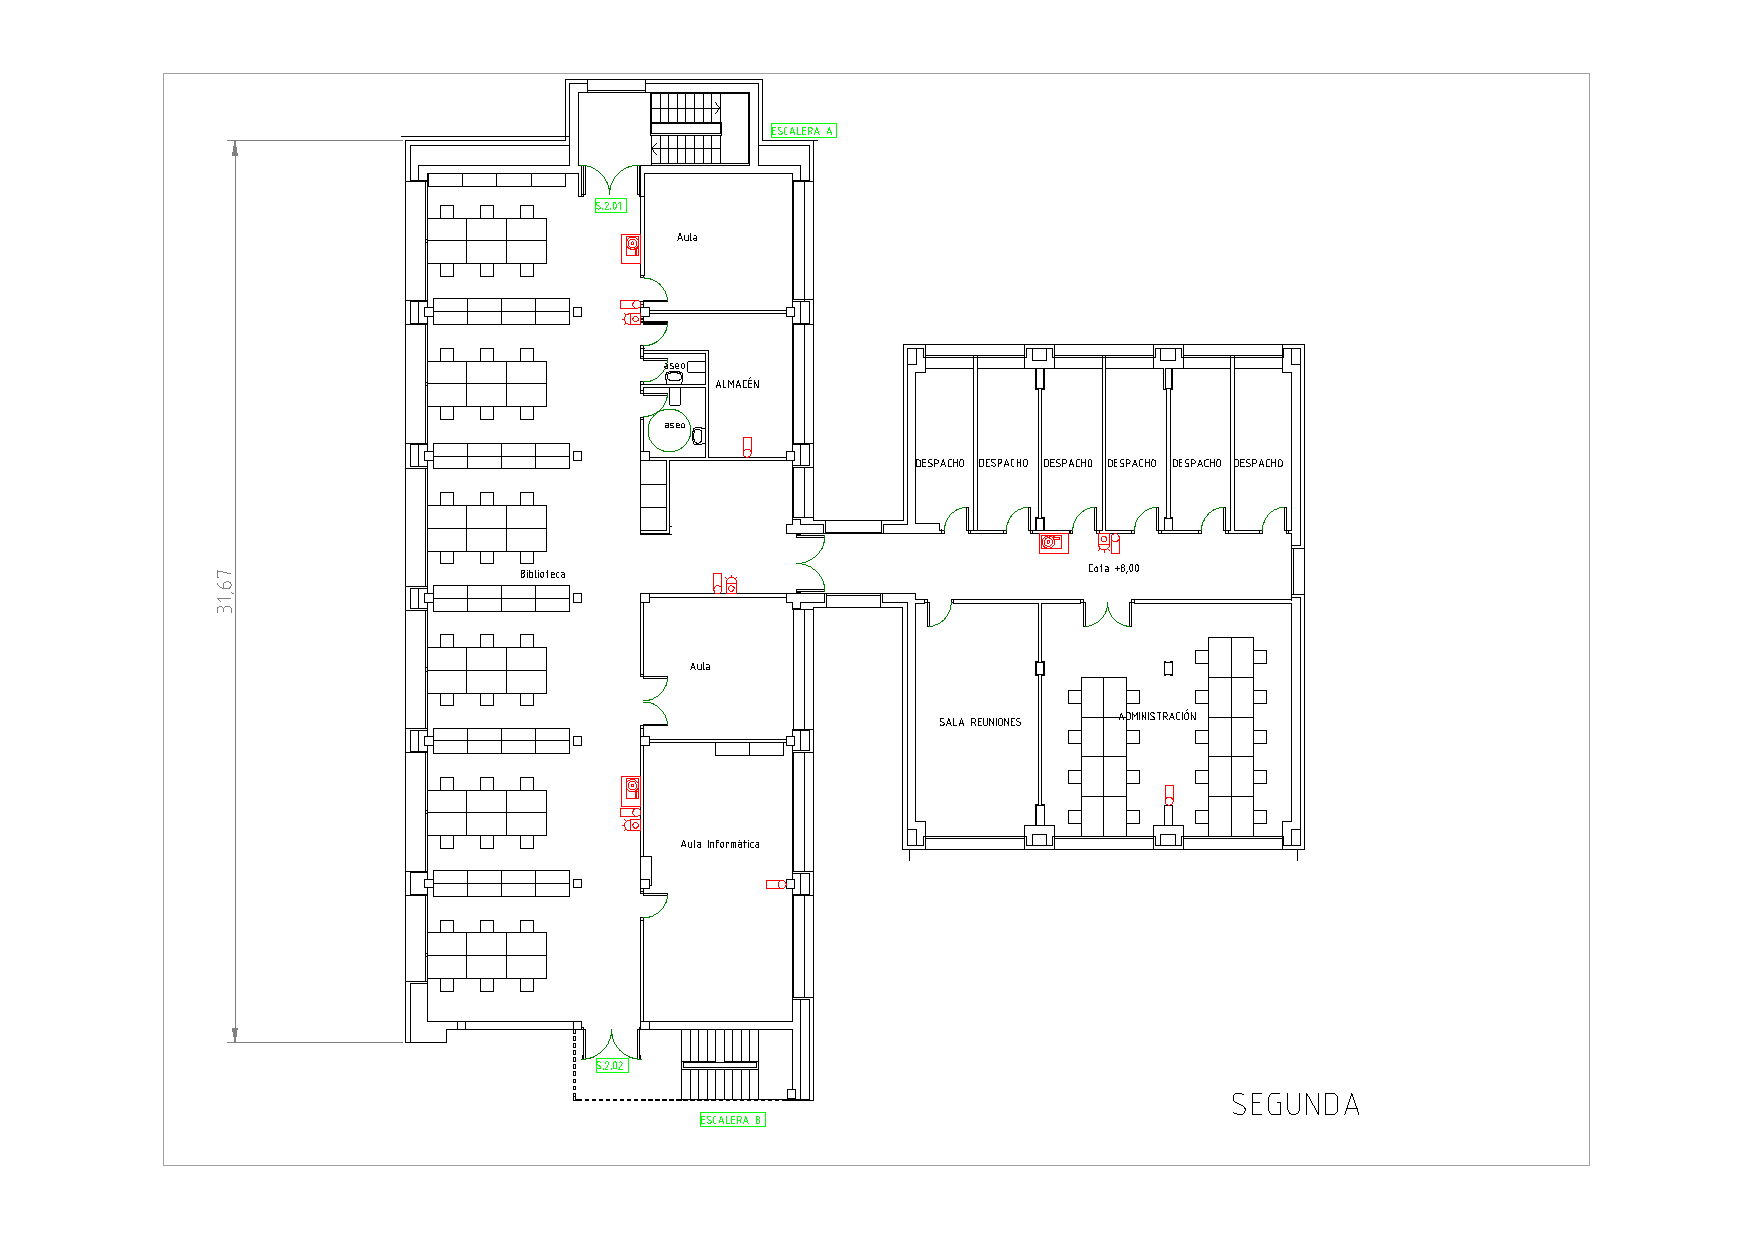
\includepdf[scale=0.95, landscape, pagecommand={}]{planos/plano-planta2.pdf}
\end{figure}
%
\conjuntoplanos{Conjunto de prácticas del Máster de Incendios repetido}
%
\plano{Planta Baja bis}
\begin{figure}
	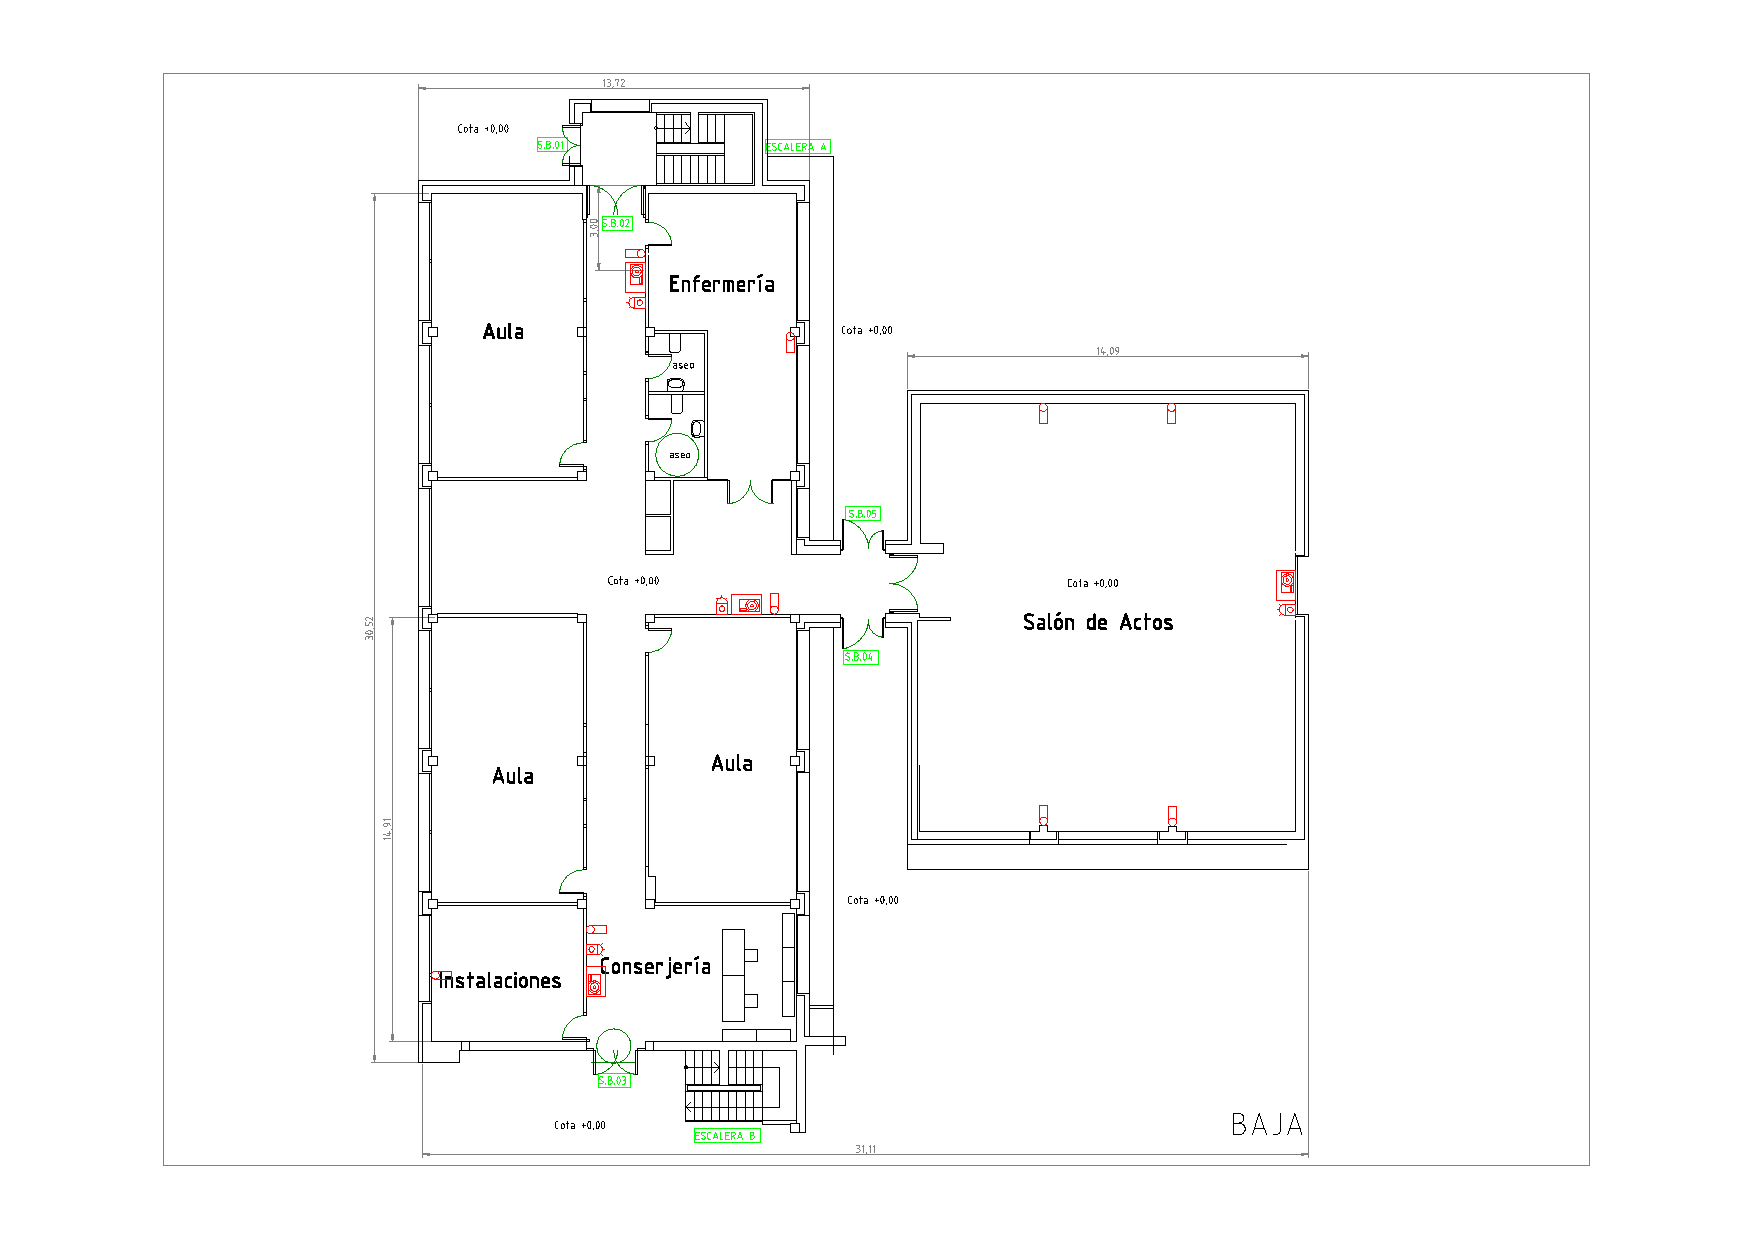
\includepdf[scale=0.95, landscape, pagecommand={}]{planos/plano-planta0.pdf}
\end{figure}
%%
\plano{Planta Primera bis}
\begin{figure}
	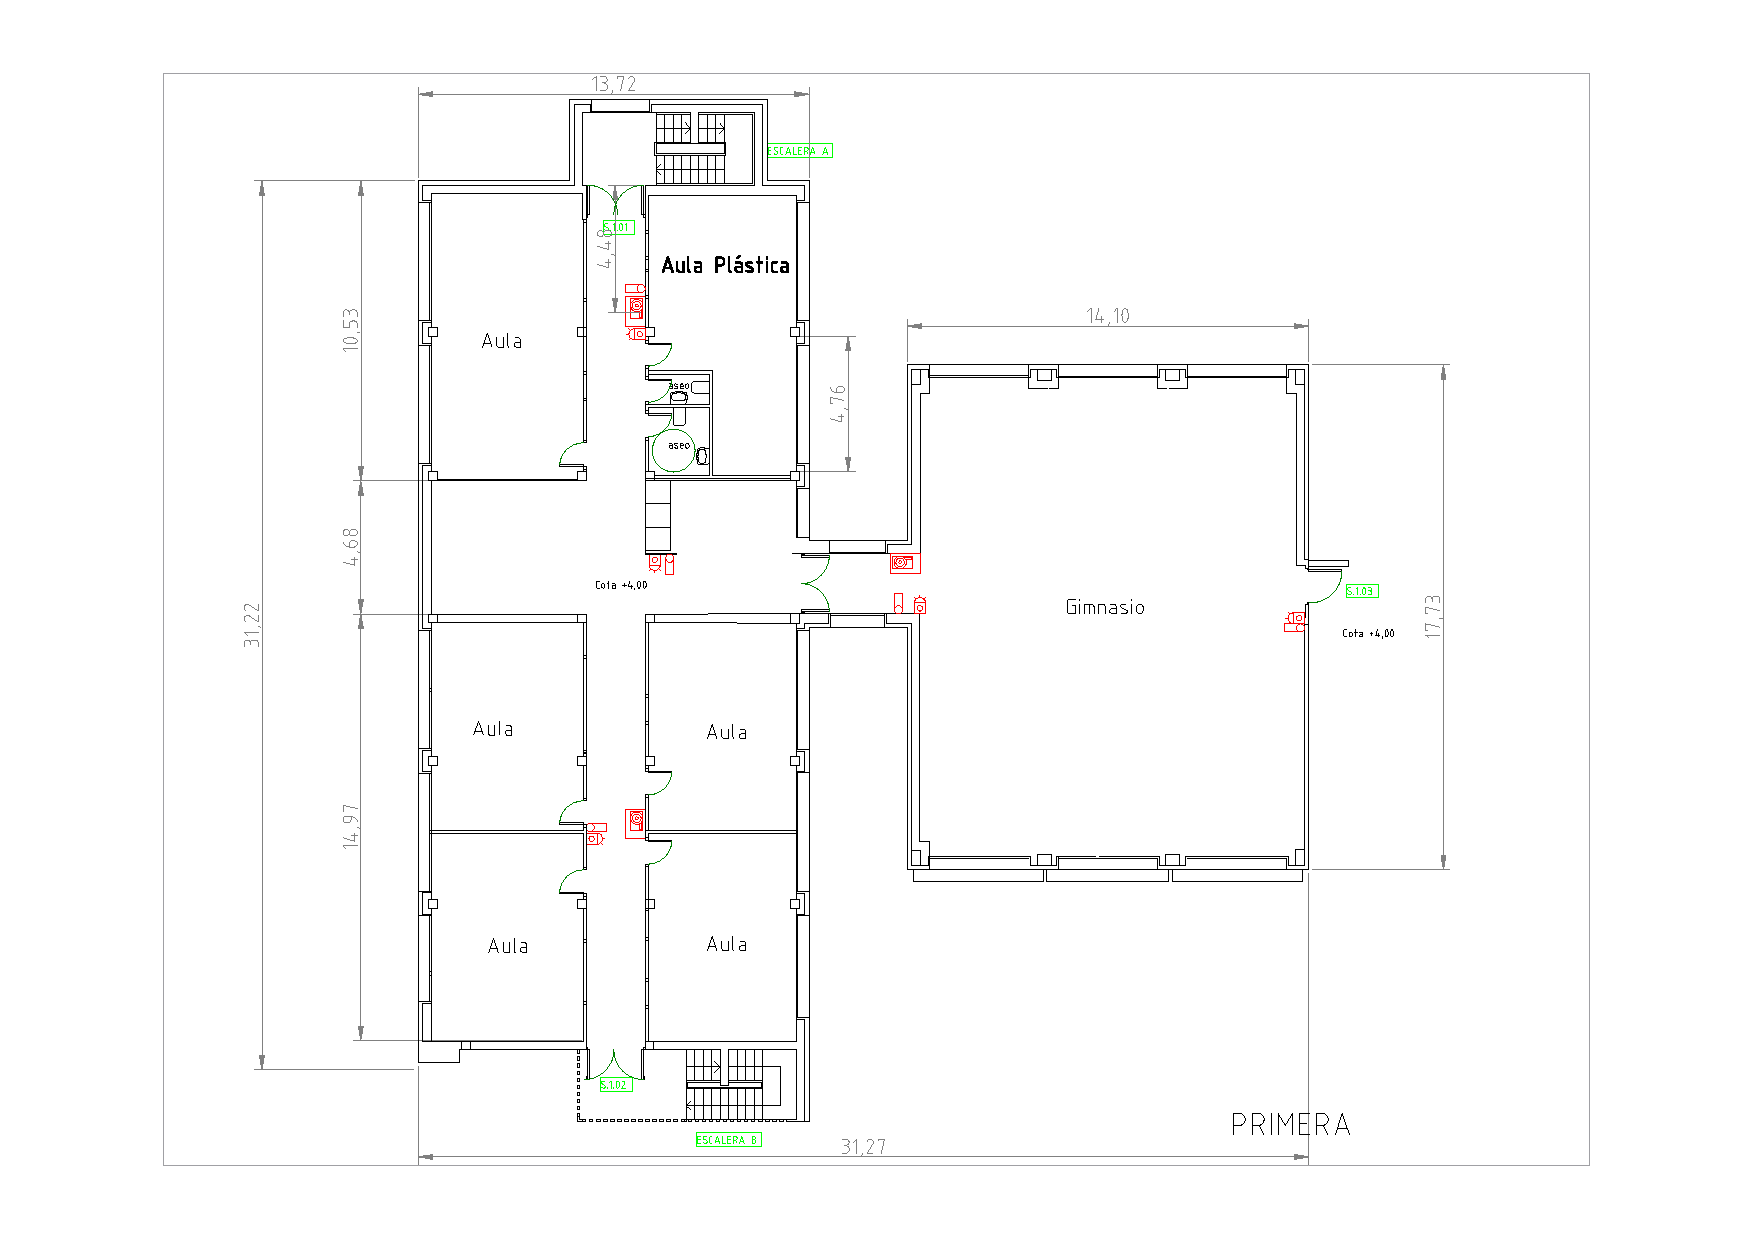
\includepdf[scale=0.95, landscape, pagecommand={}]{planos/plano-planta1.pdf}
\end{figure}
%
\plano{Planta Segunda bis}
\begin{figure}
	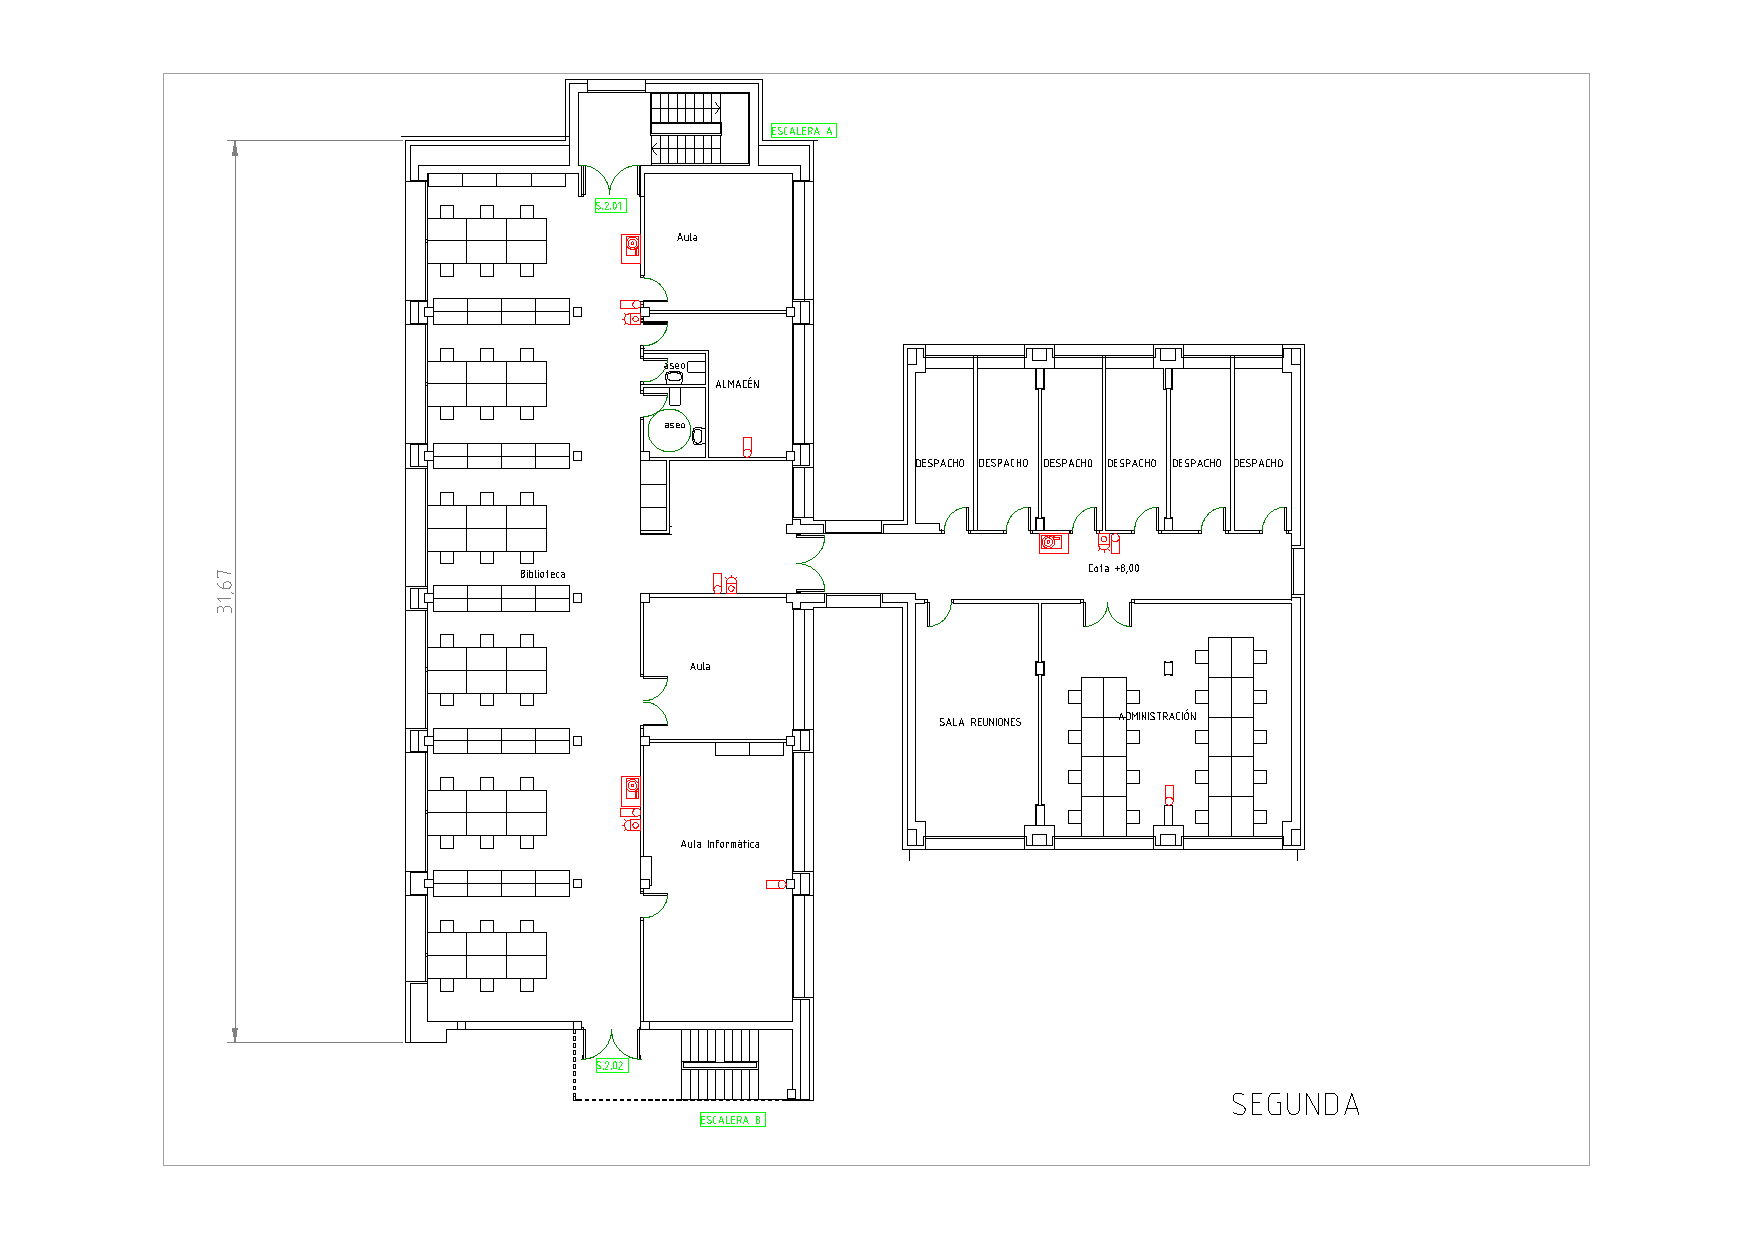
\includepdf[scale=0.95, landscape]{planos/plano-planta2.pdf}
\end{figure}
%
\addtocontents{toc}{\protect\setcounter{tocdepth}{4}}% Restaurar profundidad del ToC.
%
%--------------------------------------------------------------------------
%COD	BIBLIOGRAFÍA
%--------------------------------------------------------------------------
% Objetivo del archivo: imprimir la bibliografía; establecer los títulos y las palabras clave para segregar las referencias.
%
%--------------------------------------------------------------------------
%	BIBLIOGRAFÍA
%--------------------------------------------------------------------------
%
%	a) Por entorno BibLaTeX
% Solo es necesario especificar los comandos de impresión, ya que la información de las referencias se amacena en los archivos .BIB y se invocan en el texto.
\part{Referencias bibliográficas}
\newpage
\nocite{*}
\printbibheading[title=Referencias bibliográficas]
\printbibliography[category=cited,heading=subbibliography,title={Referencias}]
\printbibliography[notcategory=cited,notkeyword={nor},heading=subbibliography,title={Bibliografía}]
\printbibliography[notcategory=cited,keyword={nor},heading=subbibliography,title={Normativa}]
%
%--------------------------------------------------------------------------
%COD	ANEXOS
%--------------------------------------------------------------------------
% Objetivo del archivo: declarar el inicio de los anexos e incluirlos.
\appendix% Declaración de inicio de anexos. Todo lo que se incluya a partir de esta línea es parte de los anexos.%
%
%
%	------------------------------------
%COD	GLOSARIOS
%-	------------------------------------
% Al estar tras la declaración de inicio de anexos, los glosarios se consideran como anexos. Al definir cada glosario como un capítulo (\chapter) cada uno es un anexo.
% Glosario de términos:
\printunsrtglossary
% Glosario de siglas y abreviaturas:
\printunsrtglossary[type=\acronymtype, title=Siglas y Abreviaturas, toctitle=Siglas y Abreviaturas]
% Glosario de símbolos
\printunsrtglossary[type=symbols, title=Listado de símbolos, toctitle=Listado de símbolos]
%
%--------------------------------------------------------------------------
%
%--------------------------------------------------------------------------
%	CIERRE DEL \LaTeX
%--------------------------------------------------------------------------
\end{document}% Declaración de fin del \LaTeX imprimible.
%
%--------------------------------------------------------------------------
%	FIN DEL \LaTeX